\documentclass[11pt]{report}
\usepackage[a4paper, width=6.5in, height=9.2in]{geometry}
\usepackage[portuguese]{babel}
\usepackage[utf8]{inputenc}
\usepackage{listings}
\usepackage{color}
\usepackage{setspace}
\usepackage{hyperref}
\usepackage{acro}
\usepackage{amsmath}
\usepackage{amsthm}
\usepackage{graphicx}
\usepackage{subcaption}
\usepackage{cancel}
\usepackage{tikz}
\usepackage{color}
\usepackage{float}
\usepackage{titlesec}
\usepackage{todonotes}
\usepackage{minted}
\usepackage{nicematrix}
\usepackage{appendix}
\usepackage{listings}
\usepackage{xcolor}

\setmintedinline{breaklines=true, mathescape}
\lstdefinestyle{mystyle}{
    % backgroundcolor=\color{lightgray!20}, % set background color
    commentstyle=\color{green!50!black},
    keywordstyle=\color{blue!80!black},
    numberstyle=\tiny\color{gray},
    stringstyle=\color{red!80!black},
    basicstyle=\ttfamily\footnotesize,
    breakatwhitespace=false,
    breaklines=true,
    captionpos=b,
    keepspaces=true,
    numbers=left,
    numbersep=5pt,
    showspaces=false,
    showstringspaces=false,
    showtabs=false,
    tabsize=2
}

\lstset{style=mystyle}


% Comandos
\newenvironment{myminted}[1]{
    \VerbatimEnvironment
    \begin{minted}[linenos, xleftmargin=16pt, breaklines=true, breakanywhere=true, escapeinside=||]{#1}%
}{
    \end{minted}
}

\newenvironment{coloredtable}[1]{
    \begin{NiceTabular}{#1}[colortbl-like,rules/color=darkblue!50]
        \CodeBefore
            \rowcolor{darkblue}{1}
            \rowcolors{2}{lightblue!0}{lightblue}
        \Body
            \hline
}{
    \end{NiceTabular}
}


% Adiciona bibliografia ao índice
\usepackage[nottoc,notlot,notlof]{tocbibind}

% Definições - Tema minted, espaçamento, etc.
\usemintedstyle{autumn}

\setstretch{1.3}
\renewcommand{\arraystretch}{1.3}

\definecolor{darkblue}{RGB}{38,131,198}
\definecolor{lightblue}{RGB}{208,231,247}

% Ajustar o espaçamento antes de capítulos, indíce, etc.
\titleformat{\chapter}[display]{\normalfont\huge\bfseries}{\chaptertitlename\ \thechapter}{20pt}{\Huge}
\titlespacing*{\chapter}{0pt}{-16pt}{30pt}


\begin{document}

% Capa
\title{Mestrado em Engenharia Informática \\ \textbf{Bases de Dados NoSQL} \\ Trabalho Prático (23/24)}

\author{
\includegraphics[width=0.2\textwidth]{Imagens/Capa/Afonso.png} \\
            Afonso Miguel Matos Bessa \\ pg53597
        \and
        
\includegraphics[width=0.2\textwidth]{Imagens/Capa/Francisco.png} \\
            Francisco Luís Rodrigues Claudino \\ pg50380
        \and
        \includegraphics[width=0.2\textwidth]{Imagens/Capa/João Abreu.jpg} \\
            João Paulo Machado Abreu \\ pg53928
        \and
        \includegraphics[width=0.2\textwidth]{Imagens/Capa/João Faria.png} \\
            João Pedro Dias Faria \\ pg53939
        \and
        
\includegraphics[width=0.2\textwidth]{Imagens/Capa/Ricardo.png} \\
            Ricardo Cardoso Sousa \\ pg54179}

\date{\vspace{\fill} 10 de junho de 2024}


\begin{figure}[t]
    \centering
    
\includegraphics[width=0.35\textwidth]{Imagens/Capa/Logo UM.png}
    \vspace{-2.5cm}
\end{figure}

\maketitle


% Índice e Listas
\pagenumbering{roman}
\tableofcontents
%\lstlistoflistings
%\listoffigures
%\listoftables

% Capítulos
\newpage
\pagenumbering{arabic}
\chapter{Introdução}
\paragraph{}
No âmbito da unidade curricular de Bases de Dados NoSQL inserida no Mestrado em Engenharia Informática foi desenvolvido um projeto prático com o objetivo de explorar e aplicar diferentes paradigmas de bases de dados. Este projeto tem como foco a migração de dados de um sistema de gestão hospitalar baseado em \textbf{SQL} (Oracle SQL) para dois sistemas não relacionais distintos: \textbf{MongoDB}, uma base de dados orientada a documentos, e \textbf{Neo4j}, uma base de dados orientada a grafos.

A importância desta migração reside na necessidade de adaptar os sistemas de base de dados às crescentes demandas e complexidades dos dados modernos. Enquanto as bases de dados relacionais tradicionais oferecem uma estrutura rígida e tabular, as bases de dados NoSQL proporcionam flexibilidade e escalabilidade para lidar com volumes massivos de dados, estruturas variadas e relações complexas.

Ao longo deste trabalho, foram definidos processos para a migração eficaz dos dados, a implementação de consultas para demonstrar as capacidades operacionais dos sistemas implementados e uma análise crítica comparando as funcionalidades dos sistemas não relacionais com o sistema relacional original.

Este relatório técnico apresenta de forma detalhada o trabalho desenvolvido, desde a análise inicial até à implementação final dos sistemas de base de dados não relacionais, evidenciando as estratégias adotadas, os desafios enfrentados e os resultados obtidos.
\chapter{Arquitetura}
\paragraph{}

A arquitetura do projeto é representada na Figura \ref{fig:Arquitetura}. Este ilustra os caminhos de migração do \textbf{Oracle SQL} para o \textbf{MongoDB} e \textbf{Neo4j}, e destaca a fase de exploração para cada sistema de bases de dados.

\begin{itemize}
    \item \textbf{Oracle SQL}: A base de dados relacional de origem, contendo várias tabelas como pacientes, staff, episódios, entre outras, que representam os dados do hospital.
    \item \textbf{MongoDB}: Uma base de dados orientada a documentos onde os dados são armazenados em documentos flexíveis, semelhantes a JSON. Este sistema é utilizado para gerir a natureza semi-estruturada e hierárquica dos dados do hospital.
    \item \textbf{Neo4j}: Uma base de dados orientada a grafos, desenhada para gerir dados altamente conectados. É empregada para representar as relações complexas entre diferentes entidades dentro1 do sistema hospitalar.
\end{itemize}

Os principais objetivos deste projeto incluem a \textbf{Migração de Dados}, a \textbf{Exploração do Sistema} e a \textbf{Análise Crítica}. A migração de dados consiste em transferir informações de uma base de dados Oracle SQL existente, que armazena dados de um sistema de gestão hospitalar, para MongoDB e Neo4j. Este processo envolve compreender a estrutura dos dados, definir as transformações necessárias e implementar scripts para facilitar a transferência.

A exploração do sistema visa implementar um conjunto de consultas para demonstrar as capacidades operacionais dos novos sistemas não relacionais. Isto envolve investigar como os dados podem ser acedidos, manipulados e utilizados dentro do MongoDB e Neo4j, em comparação com a base de dados Oracle SQL original.

Por fim, a análise crítica foca-se em realizar uma comparação dos modelos de bases de dados relacionais e não relacionais, avaliando as vantagens, limitações e desempenho de cada sistema no tratamento dos dados do hospital.

\begin{figure}[H]
    \centering
    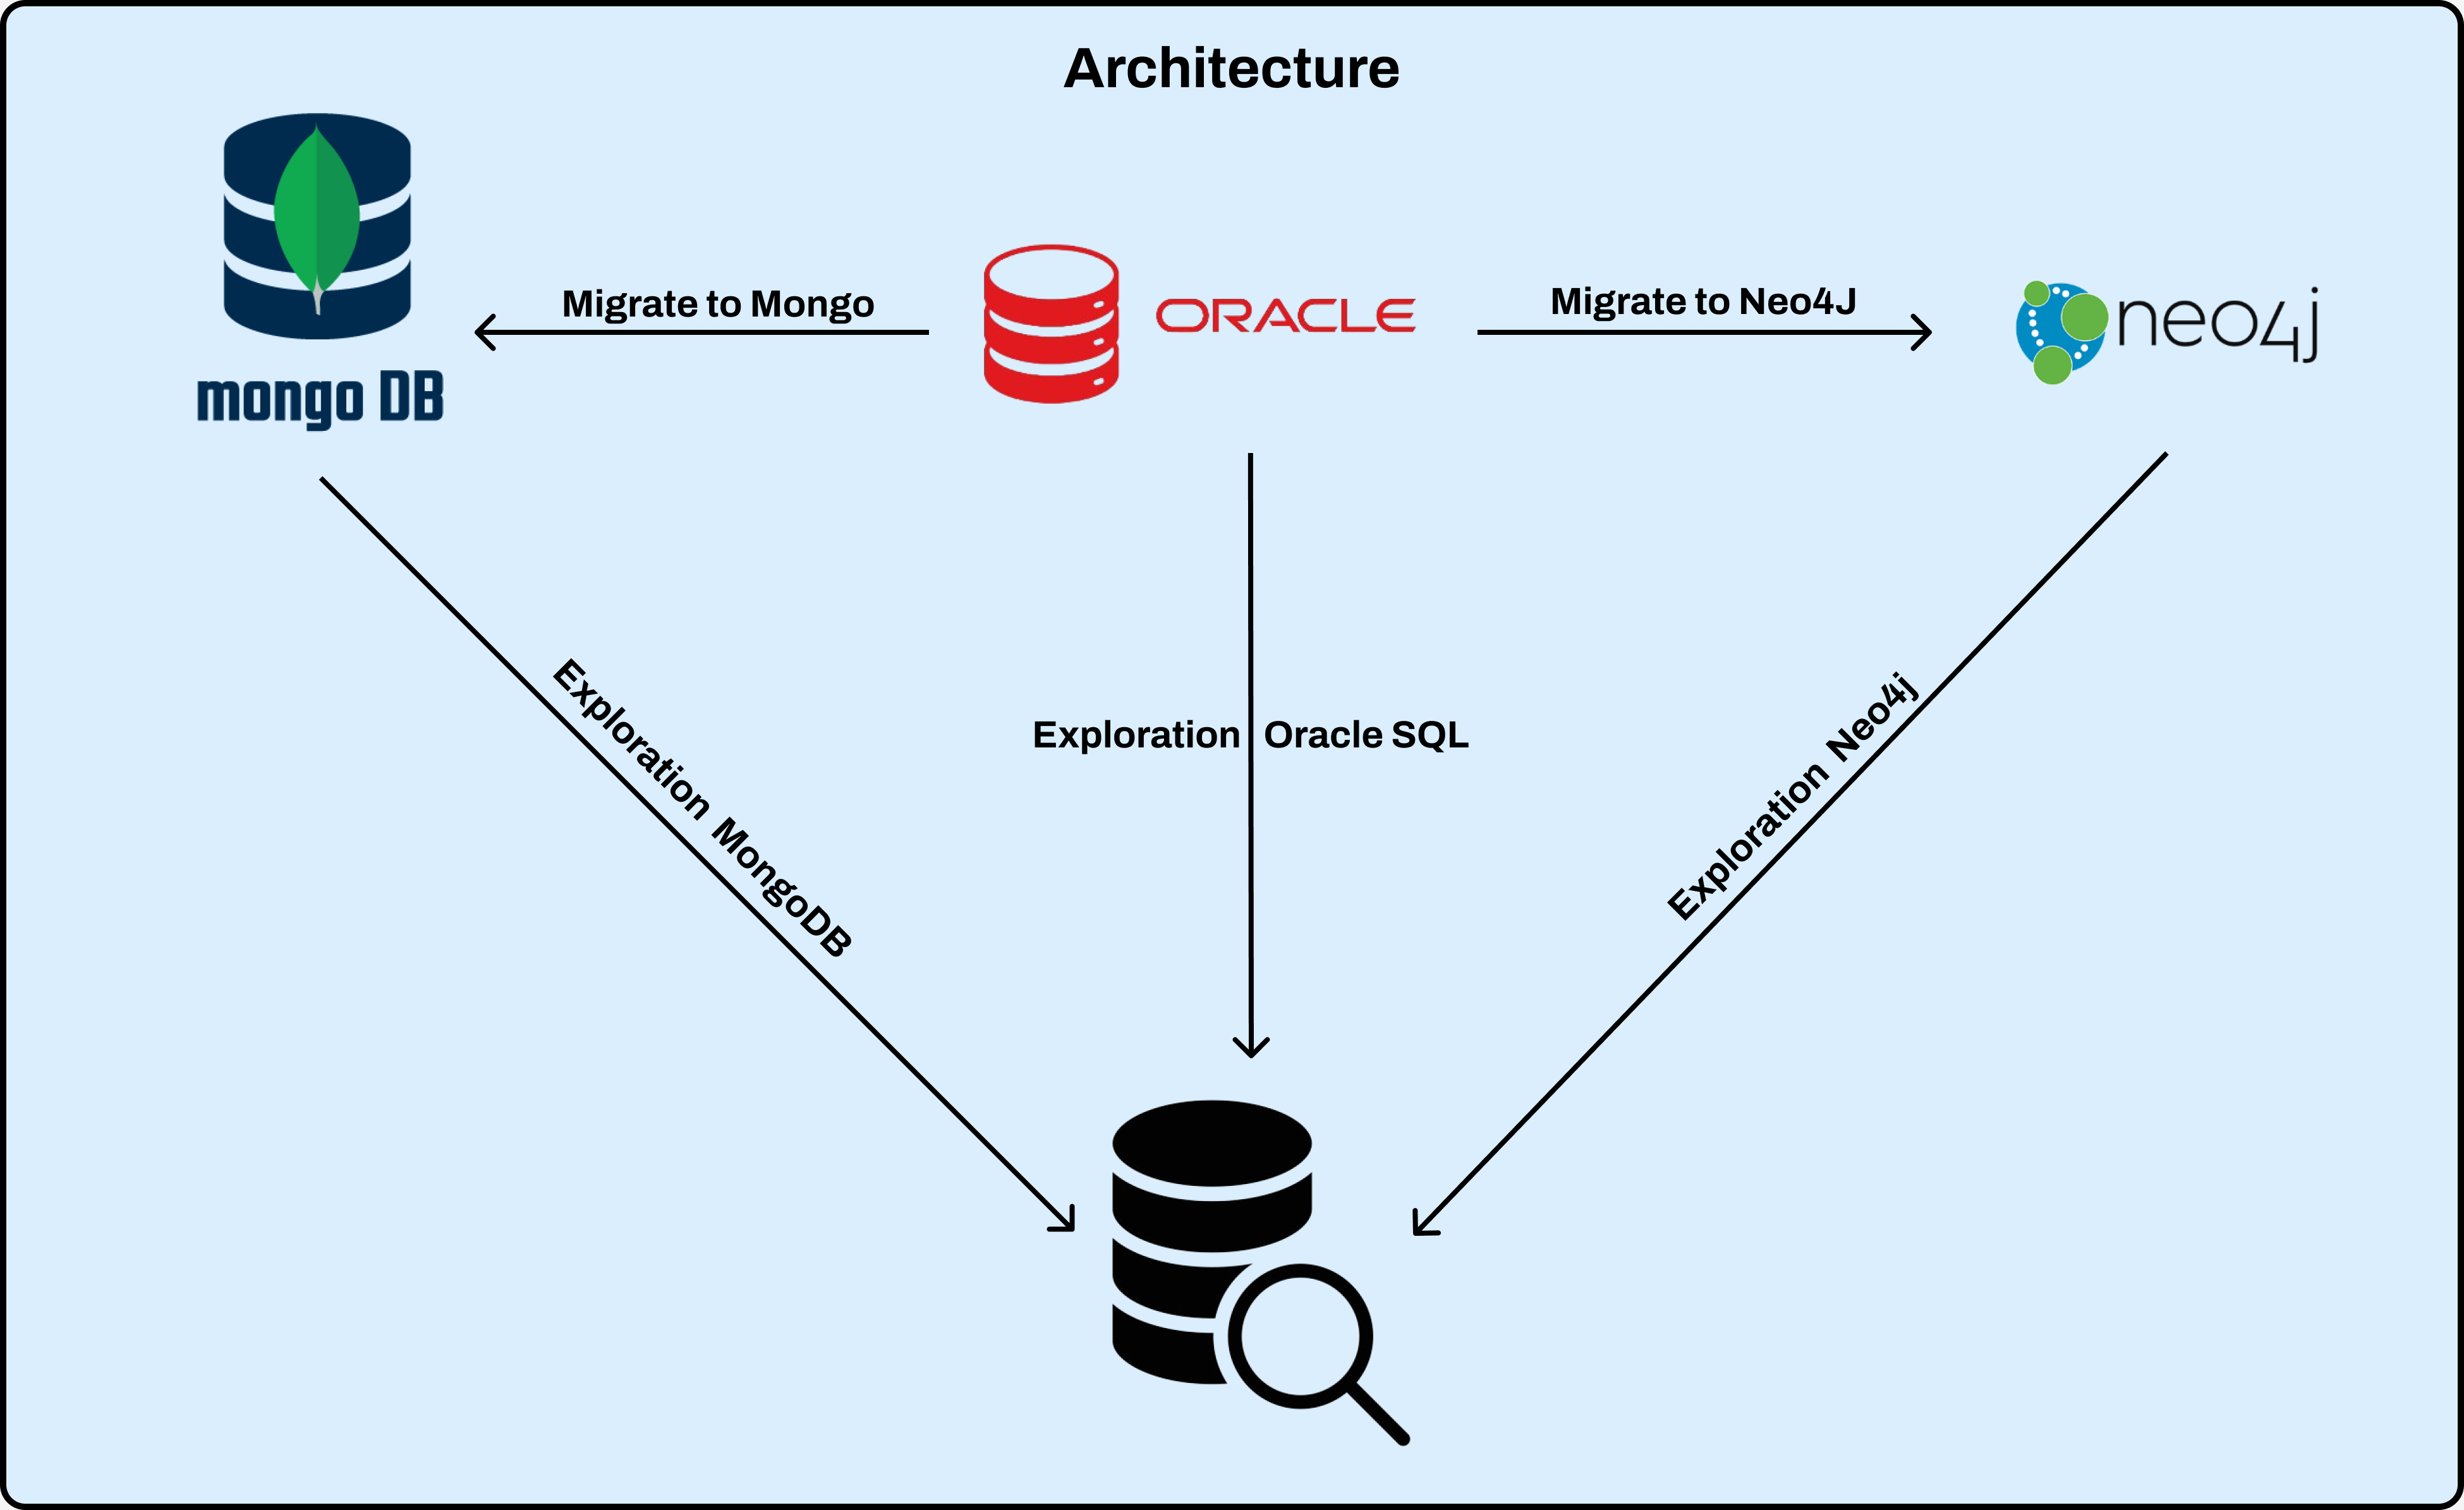
\includegraphics[width=0.8\linewidth]{Imagens/arquitetura.png}
    \caption{Arquitetura}
    \label{fig:Arquitetura}
\end{figure}


\chapter{Base de dados relacional - Oracle SQL}
\paragraph{}
A linguagem \textbf{SQL} (Structured Query Language) é um elemento central na gestão de sistemas de bases de dados relacionais, como o \textbf{Oracle SQL}. Esta linguagem permite a definição, manipulação e consulta de dados, sendo fundamental para a administração eficiente e eficaz de grandes volumes de informações. No contexto do Oracle SQL, os comandos SQL possibilitam a criação de estruturas complexas, a realização de consultas detalhadas e a implementação de regras de negócios através de procedimentos armazenados e funções.

Neste capítulo, exploraremos os princípios fundamentais do Oracle SQL aplicados ao desenvolvimento e gestão de uma base de dados para um sistema hospitalar. Abordaremos desde a criação de \textit{tablespaces}, que são \textit{containers} lógicos para armazenamento físico dos objetos de banco de dados, até a definição de utilizadores, permissões e a construção de esquemas complexos que refletem as operações diárias de uma instituição de saúde.

Para iniciar o projeto de um sistema de base de dados para um hospital, o primeiro passo foi criar um \textit{tablespace}. Um \textit{tablespace} é um \textit{container} lógico onde todos os objetos do banco de dados, como tabelas e índices, são armazenados fisicamente. Utilizámos o seguinte comando SQL para criar o \textit{tablespace}:

Assim, para iniciar o projeto de um sistema de base de dados para um sistema hospitalar, o primeiro passo foi criar um \textit{tablespace}. Um \textit{tablespace} é um \textit{container} lógico onde todos os objetos do banco de dados, como tabelas e índices, são armazenados fisicamente.

Usámos o seguinte comando SQL para criar o \textit{tablespace}:

\begin{myminted}{sql}
CREATE TABLESPACE hospital_tables
DATAFILE 'hospital_files_01.dbf'
SIZE 200M REUSE AUTOEXTEND ON
NEXT 100M MAXSIZE UNLIMITED;
\end{myminted}


Aqui, criámos um \textit{tablespace} chamado \texttt{hospital\_tables} e associámo-lhe um ficheiro de dados denominado \texttt{hospital\_files\_01.dbf}. O tamanho inicial do ficheiro de dados foi de 200 \textit{megabytes}, podendo crescer automaticamente em incrementos de 100 \textit{megabytes} até um tamanho ilimitado.

De seguida, criámos um novo utilizador chamado \textbf{hospital} com a senha \textbf{hospital}. Definimos o \texttt{hospital\_tables} como o \textit{tablespace} padrão para este utilizador e concedemos-lhe uma quota ilimitada para utilização do espaço nesse \textit{tablespace}. Utilizámos o seguinte comando:

\begin{myminted}{psql}
CREATE USER hospital IDENTIFIED BY "hospital" DEFAULT TABLESPACE hospital_tables 
QUOTA UNLIMITED ON hospital_tables;
\end{myminted}

Para que o utilizador hospital pudesse conectar-se ao banco de dados e criar objetos, concedemos os privilégios necessários com o comando:

\begin{myminted}{psql}
GRANT CONNECT, RESOURCE, CREATE VIEW TO hospital;
\end{myminted}

Após a criação do \textit{tablespace} e do utilizador, o próximo passo foi definir o esquema atual para o utilizador \textbf{Hospital} e criar as sequências, tabelas, chaves primárias (PK) e chaves estrangeiras (FK). Para isso, executamos o ficheiro \texttt{hospital.sql} que para além das estruturas da base de dados, possui também os comandos para inserir dados iniciais, como informações de pacientes, funcionários, médicos e outras entidades fundamentais para o funcionamento do sistema hospitalar.

\section{Exploração da Base de Dados}

Na etapa de exploração da base de dados relacional, o grupo optou por realizar uma subdivisão do sistema hospitalar em três grandes visões: \textbf{Pacientes}, \textbf{Staff} e \textbf{Episodes}. De referir que esta divisão foi efetuada de forma meramente académica, com o objetivo de facilitar a exploração da Base de Dados. Ajudou a compreender melhor o funcionamento do sistema hospitalar e facilitou o processo de exploração da Base de Daddos Relacional.

A primeira visão, \textbf{Pacientes}, abrange todas as informações relacionadas aos pacientes, que são acessíveis e passíveis de inserção, atualização e eliminação por parte dos utilizadores numa plataforma hospitalar. Esta categoria inclui o acesso a informações pessoais, contactos de emergência, detalhes do seguro e histórico médico.

De maneira semelhante, a segunda visão \textbf{Staff}, engloba todas as informações relativas aos membros responsáveis pelo funcionamento de uma unidade hospitalar, isto é, todos os médicos, enfermeiros e técnicos, bem como o departamento onde estes desempenham as suas funções.

Por fim, a visão \textbf{Episodes} alberga todas as informações internas do sistema hospitalar, incluindo prescrições médicas, episódios de atendimento, faturação, gestão de salas, triagem laboratorial e outras operações administrativas essenciais. Esta categoria é fundamental para assegurar a eficiência e a organização das atividades hospitalares, permitindo uma gestão integrada e eficaz de todos os recursos e processos.

No entanto, para explorar ao máximo cada detalhe existente no sistema hospitalar, será frequentemente necessário envolver uma ou mais categorias de forma a obter uma visão completa e integrada das informações. Esta abordagem cruzada dados entre \textbf{Pacientes}, \textbf{Staff} e \textbf{Episodes} possibilita uma análise mais detalhada e precisa das operações hospitalares, melhorando assim a tomada de decisões e a eficiência dos processos internos.

Virando agora o foco para a exploração em SQL, para realizar a exploração mais detalhada e pormenorizada possível, recorremos essencialmente a quatro tipos distintos de ferramentas: \textbf{Queries}, \textbf{Functions}, \textbf{Procedures} e \textbf{Triggers}.

\subsection{Queries}

Primeiramente, as \textbf{Queries} são usadas para interrogar a base de dados, permitindo a recuperação de dados específicos de acordo com critérios definidos. Estas consultas são fundamentais para obter informações precisas e rápidas sobre os diversos aspetos do sistema hospitalar, como dados de pacientes, histórico médico, disponibilidade de staff e detalhes de faturação.

Um exemplo de uma Query é apresentado abaixo:

\begin{myminted}{sql}
SELECT M.M_NAME, M.M_QUANTITY, M.M_COST
FROM Hospital.Medicine M
ORDER BY M.M_NAME;
\end{myminted}

Neste exemplo, a query seleciona o nome, quantidade e custo de todos os medicamentos armazenados na tabela \textit{Medicine}, ordenados por nome.

\subsection{Functions}

As \textbf{Functions}, por outro lado, aceitam parâmetros, o que permite uma exploração mais aprofundada e personalizada de acordo com as necessidades do utilizador. Esta flexibilidade é crucial para simular o funcionamento real de um hospital, onde as operações muitas vezes dependem de variáveis dinâmicas e requisitos específicos, como a verificação de disponibilidade de médicos ou a análise de resultados de exames laboratoriais para um dado paciente.

Um exemplo de uma Function é apresentado abaixo:

\begin{myminted}{sql}
CREATE OR REPLACE TYPE PatientInsurance_PlanRow AS OBJECT (
  IDPATIENT NUMBER(38,0),
  PATIENT_FNAME VARCHAR2(45),
  PATIENT_LNAME VARCHAR2(45),
  BLOOD_TYPE VARCHAR2(3),
  PHONE VARCHAR2(12),
  EMAIL VARCHAR2(50),
  GENDER VARCHAR2(10),
  POLICY_NUMBER VARCHAR2(45),
  BIRTHDAY DATE,
  INSURANCE_PLAN VARCHAR2(45)
);
\end{myminted}

Este excerto de código cria um tipo de objeto chamado \textit{PatientInsurance\_PlanRow}, que é uma estrutura para armazenar informações de pacientes, incluindo detalhes como nome, tipo sanguíneo, telefone, email, género, número da apólice de seguro, data de nascimento e plano de seguro. Cada campo possui um tipo de dado específico, por exemplo, \textit{IDPATIENT} é um número, \textit{PATIENT\_FNAME} é uma string de até 45 caracteres, \textit{BIRTHDAY} é uma data, entre outros.

\begin{myminted}{sql}
CREATE OR REPLACE TYPE PatientInsurance_PlanTable IS TABLE OF PatientInsurance_PlanRow;
\end{myminted}

Aqui, definimos um tipo de tabela de objetos chamado \textit{PatientInsurance\_PlanTable}. Esta tabela é uma coleção de objetos do tipo \textit{PatientInsurance\_PlanRow}, permitindo armazenar múltiplas linhas de dados de pacientes.

\begin{myminted}{sql}
CREATE OR REPLACE FUNCTION ListPatientsByInsurancePlan(plan_name IN VARCHAR2)
  RETURN PatientInsurance_PlanTable PIPELINED IS
BEGIN
  FOR rec IN (
    SELECT p.IDPATIENT, p.PATIENT_FNAME, p.PATIENT_LNAME, p.BLOOD_TYPE, p.PHONE,
           p.EMAIL, p.GENDER, p.POLICY_NUMBER, p.BIRTHDAY, i.INSURANCE_PLAN
    FROM HOSPITAL.PATIENT p
    JOIN HOSPITAL.INSURANCE i ON p.POLICY_NUMBER = i.POLICY_NUMBER
    WHERE i.INSURANCE_PLAN = plan_name
  ) LOOP
    PIPE ROW (PatientInsurance_PlanRow(
      rec.IDPATIENT, rec.PATIENT_FNAME, rec.PATIENT_LNAME, rec.BLOOD_TYPE, rec.PHONE,
      rec.EMAIL, rec.GENDER, rec.POLICY_NUMBER, rec.BIRTHDAY, rec.INSURANCE_PLAN
    ));
  END LOOP;
  RETURN;
END ListPatientsByInsurancePlan;
\end{myminted}

Esta função, \textit{ListPatientsByInsurancePlan}, aceita um parâmetro \textit{plan\_name} do tipo \textit{VARCHAR2} e retorna uma tabela de objetos \textit{PatientInsurance\_PlanTable}. A função usa um loop \textit{FOR} para iterar sobre os resultados de uma consulta que seleciona informações de pacientes a partir das tabelas \textit{PATIENT} e \textit{INSURANCE}, onde o plano de seguro corresponde ao valor fornecido em \textit{plan\_name}. Para cada linha resultante, a função usa \textit{PIPE ROW} para adicionar um objeto \textit{PatientInsurance\_PlanRow} à tabela resultante, que contém os dados do paciente.

\begin{myminted}{sql}
SELECT * FROM TABLE(ListPatientsByInsurancePlan('Standard Plan'));
\end{myminted}

Esta consulta executa a função \textit{ListPatientsByInsurancePlan} passando o valor \textit{Standard Plan} como argumento. O resultado é uma tabela com todas as informações dos pacientes que estão no plano de seguro.

Cada parte deste código SQL trabalha em conjunto para permitir a criação e utilização de uma função que retorna dados estruturados de pacientes com base no plano de seguro. Isso facilita a personalização e a flexibilidade ao consultar dados em um cenário de hospital real.

\subsection{Procedures}

As \textbf{Procedures} são blocos de código armazenados que executam uma série de operações SQL de forma automatizada. Estas são particularmente úteis para realizar tarefas repetitivas e complexas de forma eficiente, como a atualização de registos de pacientes, o processamento de faturações e a gestão de inventário de medicamentos. As Procedures permitem a automação de processos críticos, garantindo a consistência e a integridade dos dados ao longo do tempo.

Embora as Views sejam úteis para simplificar consultas complexas e melhorar a segurança ao restringir colunas visíveis, elas têm limitações significativas em comparação com as Procedures. As Views não permitem lógica condicional ou controlos avançados de fluxo, têm capacidades limitadas para operações de escrita complexas, e podem introduzir overhead de performance em consultas complexas. As Procedures, por outro lado, são mais flexíveis e eficientes para automação de processos críticos, permitindo encapsular lógica de negócios complexa, realizar operações de escrita robustas e otimizar performance, além de facilitar a manutenção e reutilização do código. Portanto, para tarefas repetitivas e complexas, as Procedures são uma escolha mais adequada do que as Views.

Um exemplo de uma Procedure é apresentado abaixo:

\begin{myminted}{sql}
DECLARE
    max_id NUMBER;
BEGIN
    SELECT COALESCE(MAX(IDPATIENT), 0) INTO max_id FROM Hospital.PATIENT;

    BEGIN
        EXECUTE IMMEDIATE 'DROP SEQUENCE patient_seq_new';
    EXCEPTION
        WHEN OTHERS THEN
            IF SQLCODE != -2289 THEN
                RAISE;
            END IF;
    END;
\end{myminted}

No primeiro bloco, declaramos uma variável \textit{max\_id} para armazenar o valor máximo atual da coluna \textit{IDPATIENT} na tabela \textit{Patient}. Usamos a função \textit{COALESCE} para garantir que, caso não haja registos, \textit{max\_id} seja definido como 0. Em seguida, usamos \textit{EXECUTE IMMEDIATE} para criar uma nova sequência chamada \textit{patient\_seq\_new}, que começa a partir do valor \textit{max\_id + 1} e incrementa por 1 para cada novo registo. Esta sequência é usada para gerar IDs únicos para novos pacientes, evitando conflitos de chave primária.

\begin{myminted}{sql}
CREATE OR REPLACE PROCEDURE insert_patient (
    p_patient_fname VARCHAR2,
    p_patient_lname VARCHAR2,
    p_blood_type    VARCHAR2,
    p_phone         VARCHAR2,
    p_email         VARCHAR2,
    p_gender        VARCHAR2,
    p_birthday      DATE,
    p_policy_number VARCHAR2,
    p_condition     VARCHAR2,
    p_record_date   DATE,
    p_contact_name  VARCHAR2,
    p_contact_phone VARCHAR2,
    p_contact_relation VARCHAR2,
    p_provider      VARCHAR2,
    p_insurance_plan VARCHAR2,
    p_co_pay        NUMBER,
    p_coverage      VARCHAR2,
    p_maternity     CHAR,
    p_dental        CHAR,
    p_optical       CHAR
) IS
    v_idpatient NUMBER;
BEGIN
    INSERT INTO Hospital.PATIENT (
        IDPATIENT, PATIENT_FNAME, PATIENT_LNAME, BLOOD_TYPE, PHONE, EMAIL, GENDER, BIRTHDAY, POLICY_NUMBER
    )
    VALUES (
        patient_seq_new.NEXTVAL, p_patient_fname, p_patient_lname, p_blood_type, p_phone, p_email, p_gender, p_birthday, p_policy_number
    )
    RETURNING IDPATIENT INTO v_idpatient;

    INSERT INTO Hospital.MEDICAL_HISTORY (
        RECORD_ID, CONDITION, RECORD_DATE, IDPATIENT
    )
    VALUES (
        patient_seq_new.NEXTVAL, p_condition, p_record_date, v_idpatient
    );

    INSERT INTO Hospital.INSURANCE (
        POLICY_NUMBER, PROVIDER, INSURANCE_PLAN, CO_PAY, COVERAGE, MATERNITY, DENTAL, OPTICAL
    )
    VALUES (
        p_policy_number, p_provider, p_insurance_plan, p_co_pay, p_coverage, p_maternity, p_dental, p_optical
    );

    INSERT INTO Hospital.EMERGENCY_CONTACT (
        CONTACT_NAME, PHONE, RELATION, IDPATIENT
    )
    VALUES (
        p_contact_name, p_contact_phone, p_contact_relation, v_idpatient
    );

    DBMS_OUTPUT.PUT_LINE('Patient and related records inserted successfully.');
EXCEPTION
    WHEN OTHERS THEN
        DBMS_OUTPUT.PUT_LINE('Error: ' || SQLERRM);
END;
\end{myminted}

No segundo bloco, criamos a Procedure \textit{insert\_patient}, que aceita vários parâmetros como o primeiro nome do paciente, apelido, tipo de sangue, email, telefone, género, número de apólice, data de nascimento e vários outro relacionado ao Paciente. Dentro da Procedure, usamos o comando \textit{INSERT INTO} para adicionar um novo registo na tabela \textit{Patient}, \textit{Medical\_History}, \textit{Insurance} e  \textit{Emergency\_Contact}, utilizando \textit{patient\_seq\_new.NEXTVAL} para definir o \textit{IDPATIENT} automaticamente. A data de nascimento é convertida para o formato de data apropriado usando \textit{TO\_DATE}. Após a inserção, uma mensagem de sucesso é exibida com \textit{DBMS\_OUTPUT.PUT\_LINE}. Caso ocorra algum erro, a exceção é capturada e uma mensagem de erro é exibida com os detalhes.

Esta abordagem combinada de Queries, Functions e Procedures proporciona uma exploração robusta e abrangente do sistema hospitalar, garantindo que todas as informações necessárias estejam acessíveis e possam ser manipuladas conforme necessário para suportar a gestão eficiente e eficaz.

\subsection{Triggers}

Finalmente, os \textbf{Triggers} em Oracle SQL são um tipo especial de procedimento armazenado que é automaticamente executado (ou "disparado") pelo Oracle Database em resposta a certos eventos em uma tabela ou visão. Os triggers são usados para aplicar regras de negócios de forma automática, manter a integridade dos dados, realizar auditoria de alterações, e implementar outras funcionalidades automáticas que não podem ser facilmente realizadas apenas com comandos SQL simples. Um exemplo de um Trigger implementado é apresentado abaixo:

\begin{myminted}{sql}
CREATE TABLE Hospital.New_Patient_Requests (
    request_id NUMBER GENERATED BY DEFAULT AS IDENTITY PRIMARY KEY,
    patient_fname VARCHAR2(45),
    patient_lname VARCHAR2(45),
    blood_type    VARCHAR2(3),
    phone         VARCHAR2(12),
    email         VARCHAR2(50),
    gender        VARCHAR2(10),
    birthday      DATE,
    policy_number VARCHAR2(45),
    condition     VARCHAR2(45),
    record_date   DATE,
    contact_name  VARCHAR2(45),
    contact_phone VARCHAR2(30),
    contact_relation VARCHAR2(45),
    provider      VARCHAR2(45),
    insurance_plan VARCHAR2(45),
    co_pay        NUMBER,
    coverage      VARCHAR2(20),
    maternity     CHAR(1),
    dental        CHAR(1),
    optical       CHAR(1)
);
\end{myminted}

\begin{myminted}{sql}
CREATE OR REPLACE TRIGGER trg_insert_patient
AFTER INSERT ON Hospital.New_Patient_Requests
FOR EACH ROW
BEGIN
    insert_patient(
        :NEW.patient_fname,
        :NEW.patient_lname,
        :NEW.blood_type,
        :NEW.phone,
        :NEW.email,
        :NEW.gender,
        :NEW.birthday,
        :NEW.policy_number,
        :NEW.condition,
        :NEW.record_date,
        :NEW.contact_name,
        :NEW.contact_phone,
        :NEW.contact_relation,
        :NEW.provider,
        :NEW.insurance_plan,
        :NEW.co_pay,
        :NEW.coverage,
        :NEW.maternity,
        :NEW.dental,
        :NEW.optical
    );
END;
\end{myminted}

O trigger \textit{trg\_insert\_patient} foi criado para automatizar a inserção de um novo paciente e seus registos relacionados (como historial médico, seguro e contacto de emergência) na base de dados do hospital. Ele é disparado automaticamente após a inserção de um novo pedido de paciente na tabela \textit{Hospital.New\_Patient\_Requests}.

No primeiro bloco, criamos a tabela \textit{Hospital.New\_Patient\_Requests} que é definida para armazenar pedidos de novos pacientes. Esta tabela contém informações detalhadas sobre o paciente, incluindo nome, tipo sanguíneo, contacto, seguro, entre outros. Cada coluna da tabela armazena uma informação específica sobre o paciente.

No segundo bloco, o trigger é definido para ser disparado após uma inserção (\textit{AFTER INSERT}) na tabela \textit{Hospital.New\_Patient\_Requests}. Para cada linha inserida (\textit{FOR EACH ROW}), o trigger chama o procedimento \textit{insert\_patient} previamente mencionado e descrito com os valores dos novos registos inseridos.

É importante referir que os triggers oferecem várias vantagens no contexto dos procedimentos de inserção, atualização e remoção de dados específicos, neste caso na automatização da inserção de um novo paciente e seus registos associados. Algumas das principais vantagens prendem-se com a \textbf{Redução de Erros Manuais} que, ao automatizar a inserção dos dados do paciente e os seus registos relacionados, o trigger elimina a possibilidade de erros humanos que poderiam ocorrer durante a inserção manual de dados em múltiplas tabelas. Outra das principais vantages consiste na \textbf{Consistência de Dados} pois o trigger garante que todas as informações relacionadas ao paciente sejam inseridas de forma consistente e simultânea nas tabelas apropriadas (\textit{Hospital.PATIENT}, \textit{Hospital.MEDICAL\_HISTORY}, \textit{Hospital.INSURANCE}, \textit{Hospital.EMERGENCY\_CONTACT}), algo que é fundamental numa Base de Dados Relacional.

\subsection{Queries, Functions, Procedures e Triggers implementados}

De seguida, iremos apresentar todas as explorações implementadas, bem como uma explicação detalhada de cada uma das ferramentas implementadas, para as três visões mencionadas acima, bem como para a visão global da Base de Dados que engloba sempre duas ou mais visões.

\subsubsection{Visão Pacientes}

Na visão dos pacientes, o nosso foco foi extrair as informações necessárias para o funcionamento de um hospital real. Extraímos todos os dados relacionados a pacientes específicos, além de tratar da inserção, atualização e remoção dessas informações na base de dados.

No processo de inserção, desenvolvemos um procedimento que insere informações de um novo paciente em todas as quatro tabelas da base de dados. Consideramos que não faria sentido inserir os dados em apenas uma tabela, pois isso não reflete a realidade de um hospital.

Para a atualização, permitimos que qualquer tabela relacionada a pacientes possa ser atualizada. Por exemplo, pode ser necessário atualizar apenas o contato de emergência de um paciente ou realizar uma atualização no seu histórico médico.

No que diz respeito à remoção, criamos um procedimento que remove todas as informações do paciente de todas as tabelas relevantes. Além disso, o procedimento redefine o ID do paciente na tabela de Episódios para zero. Optamos por não excluir o episódio, pois a preservação dos dados históricos é fundamental numa base de dados relacional.

Associados aos procedimentos de Inserção, Atualização e Remoção, foram desenvolvidos Triggers para que se tenha conhecimento de todos o tipo de alterações aos dados da Base de Dados, para garantir a consistência dos dados.

\vspace{0.15cm}
\textbf{AllInfoPatient:} Função que retorna todas as informações sobre um paciente específico dado o ID do paciente. A função usa uma tabela pipelined para iterar sobre os registos de pacientes e retornar cada linha como um objeto PatientRow.

\vspace{0.15cm}
\textbf{AllInfoMedicalHistory:} Função que retorna todos os registos do historial médico para um paciente específico dado o ID do paciente. A função usa uma tabela pipelined para iterar sobre os registos de histórico médico e retornar cada linha como um objeto MedicalHistoryRow.

\vspace{0.15cm}
\textbf{AllInfoInsurance:} Função que retorna todas as informações sobre o seguro de um paciente específico dado o número da apólice. A função usa uma tabela pipelined para iterar sobre os registros de seguro e retornar cada linha como um objeto InsuranceRow.

\vspace{0.15cm}
\textbf{AllInfoEmergencyContact:} Função que tetorna todas as informações sobre os contatos de emergência de um paciente específico, dado o ID do paciente. A função usa uma tabela pipelined para iterar sobre os registros de contatos de emergência e retornar cada linha como um objeto EmergencyContactRow.

\vspace{0.15cm}
 \textbf{AllInfoPatient:} Função que Retorna todas as informações combinadas de um paciente específico, dado o ID do paciente. A função junta dados de várias tabelas (paciente, histórico médico, seguro e contato de emergência) e retorna cada linha como um objeto PatientAllInfoRow.
 
\vspace{0.15cm}
\textbf{AllInfoPatientByBloodType:} Função que retorna todas as informações dos pacientes que possuem um determinado grupo sanguíneo. A função usa uma tabela pipelined para iterar sobre os registros de pacientes e retornar cada linha como um objeto PatientRow.

\vspace{0.15cm}
\textbf{AllInfoPatientByGender:} Função que retorna todas as informações dos pacientes que possuem um determinado gênero. A função usa uma tabela pipelined para iterar sobre os registros de pacientes e retornar cada linha como um objeto PatientRow.

\vspace{0.15cm}
\textbf{GetPatientsWithCondition:} Função que retorna todas as informações dos pacientes que possuem uma condição médica específica. A função usa uma tabela pipelined para iterar sobre os registros de pacientes e histórico médico, retornando cada linha como um objeto PatientRow.

\vspace{0.15cm}
\textbf{ListAllRelationsProc:} Procedimento que lista todos os tipos de relações de contato de emergência distintos na tabela de contatos de emergência.

\vspace{0.15cm}
\textbf{ListAllProvidersProc:} Procedimento que lista todos os providenciadores de seguro distintos na tabela de seguros.

\vspace{0.15cm}
\textbf{ListAllInsurancePlansProc:} Procedimento que lista todos os planos de seguro distintos na tabela de seguros.

\vspace{0.15cm}
\textbf{ListAllCoveragesProc:} Procedimento que lista todos os tipos de cobertura distintos na tabela de seguros.

\vspace{0.15cm}
\textbf{ListAllConditionsProc:} Procedimento que lista todas as condições médicas distintas na tabela de histórico médico.

\vspace{0.15cm}
\textbf{ListAllBloodTypesProc:} Procedimento que lista todos os tipos de sangue distintos na tabela de pacientes.

\vspace{0.15cm}
\textbf{ListPatientsByMedicalHistoryDate:} Função que retorna todos os pacientes que possuem registos de historial médico em uma data específica.

\vspace{0.15cm}
\textbf{ListPatientsByInsurancePlan:} Função que retorna todos os pacientes que possuem um plano de seguro específico.

\vspace{0.15cm}
\textbf{ListPatientsByCoverage:} Função que retorna todos os pacientes que possuem uma cobertura específica.

\vspace{0.15cm}
\textbf{ListPatientsByAgeRange:} Função que retorna todos os pacientes dentro de uma faixa etária específica.

\vspace{0.15cm}
\textbf{ListPatientsWithMaternityCoverageProc:} Procedimento  que retorna todos os pacientes que possuem cobertura de maternidade no seu plano de seguro.

\vspace{0.15cm}
\textbf{ListPatientsWithDentalCoverage:} Função que retorna todos os pacientes que possuem cobertura dental no seu plano de seguro.

\vspace{0.15cm}
\textbf{ListPatientsWithOpticalCoverageProc:} Procedimento que retorna todos os pacientes que possuem cobertura óptica no seu plano de seguro.

\vspace{0.15cm}
\textbf{GetPatientCountPerBloodTypeProc:} Procedimento que conta o número de pacientes para cada tipo sanguíneo distinto na tabela de pacientes.

\vspace{0.15cm}
\textbf{GetPatientCountPerConditionProc:} Procedimento que conta o número de pacientes para cada condição médica distinta na tabela de historial médico.

\vspace{0.15cm}
\textbf{insert\_patient:} Procedimento que insere um novo paciente e os registos relacionados de historial médico, seguro e contacto de emergência no banco de dados.

\vspace{0.15cm}
\textbf{trg\_insert\_patient:} Trigger que chama o procedimento \textit{insert\_patient} após a inserção de um novo pedido de paciente na tabela \textit{New\_Patient\_Requests}.

\vspace{0.15cm}
\textbf{update\_patient:} Procedimento que atualiza os detalhes de um paciente na tabela de pacientes.

\vspace{0.15cm}
\textbf{trg\_update\_patient:} Trigger que chama o procedimento \textit{update\_patient} antes de uma atualização na tabela de pacientes.

\vspace{0.15cm}
\textbf{update\_medical\_history:} Procedimento que atualiza os detalhes do historial médico de um paciente.

\vspace{0.15cm}
\textbf{trg\_update\_medical\_history:} Trigger que chama o procedimento \textit{update\_medical\_history} antes de uma atualização na tabela de historial médico.

\vspace{0.15cm}
\textbf{update\_insurance:}Procedimento que atualiza os detalhes do seguro de um paciente.

\vspace{0.15cm}
\textbf{trg\_update\_insurance:} Trigger que chama o procedimento \textit{update\_insurance} antes de uma atualização na tabela de seguros.

\vspace{0.15cm}
\textbf{update\_emergency\_contact:} Procedimento que atualiza os detalhes do contacto de emergência de um paciente.

\vspace{0.15cm}
\textbf{trg\_update\_emergency\_contact:} Trigger que chama o procedimento \textit{update\_emergency\_contact} antes de uma atualização na tabela de contactos de emergência.

\vspace{0.15cm}
\textbf{delete\_patient\_and\_related:} Procedimento que elimina um paciente e todos os registos relacionados de historial médico, seguro e contacto de emergência. Também define o ID do paciente para 0 na tabela de episódios.

\vspace{0.15cm}
\textbf{trg\_delete\_patient\_and\_related:} Trigger que chama o procedimento \textit{delete\_patient\_and\_related} antes de uma eliminação na tabela de pacientes.™

\subsubsection{Visão Staff}

Na visão do staff, o nosso foco foi extrair as informações necessárias para o funcionamento de um hospital real. Extraímos todos os dados relacionados aos funcionários, além de tratar da inserção, atualização e remoção dessas informações na base de dados.

No processo de inserção, desenvolvemos procedimentos que permitem a inclusão de novos membros do staff nas tabelas relevantes da base de dados. Consideramos que é essencial garantir que todas as informações importantes sobre um novo funcionário estejam devidamente registadas, refletindo a realidade operacional de um hospital.

Para a atualização, permitimos que qualquer tabela relacionada ao staff possa ser atualizada. Por exemplo, pode ser necessário atualizar apenas o contacto de um funcionário, ajustar suas qualificações ou alterar sua designação. Nosso objetivo foi garantir que todas as informações possam ser mantidas precisas e atualizadas de maneira eficiente.

No que diz respeito à remoção, criamos procedimentos que removem todas as informações de um funcionário das tabelas relevantes. Além disso, garantimos que quaisquer referências a esse funcionário em outras tabelas, mais concretamente o ID, seja redefinido para 0 ao invés da remoção. Optamos por não excluir dados históricos, como registos de atendimento ou episódios, para preservar a integridade e a continuidade dos dados históricos.

Tal como na visão acima, associados aos procedimentos de Inserção, Atualização e Remoção, foram desenvolvidos Triggers para que se tenha conhecimento de todos o tipo de alterações aos dados da Base de Dados, para garantir a consistência dos dados.

\vspace{0.15cm}
\textbf{AllInfoStaff:} Função que retorna todas as informações sobre um funcionário específico dado o ID do funcionário. A função usa uma tabela pipelined para iterar sobre os registos de funcionários e retornar cada linha como um objeto StaffRow.

\vspace{0.15cm}
\textbf{AllInfoDepartment:} Função que retorna todas as informações sobre um departamento específico dado o ID do funcionário. A função usa uma tabela pipelined para iterar sobre os registos de departamentos e retornar cada linha como um objeto DepartmentRow.

\vspace{0.15cm}
\textbf{AllInfoNurse:} Função que retorna todas as informações sobre uma enfermeira específica dado o ID do funcionário. A função usa uma tabela pipelined para iterar sobre os registos de enfermeiras e retornar cada linha como um objeto NurseRow.

\vspace{0.15cm}
\textbf{AllInfoDoctor:} Função que retorna todas as informações sobre um médico específico dado o ID do médico. A função usa uma tabela pipelined para iterar sobre os registos de médicos e retornar cada linha como um objeto DoctorRow.

\vspace{0.15cm}
\textbf{AllInfoTechnician:} Função que retorna todas as informações sobre um técnico específico dado o ID do funcionário. A função usa uma tabela pipelined para iterar sobre os registos de técnicos e retornar cada linha como um objeto TechnicianRow.

\vspace{0.15cm}
\textbf{AllInfoStaffByDateJoining:} Função que retorna todas as informações sobre funcionários que se juntaram numa data específica. A função usa uma tabela pipelined para iterar sobre os registos de funcionários e retornar cada linha como um objeto StaffRow.

\vspace{0.15cm}
\textbf{AllInfoStaffByDateSeperation:} Função que retorna todas as informações sobre funcionários que se separaram numa data específica. A função usa uma tabela pipelined para iterar sobre os registos de funcionários e retornar cada linha como um objeto StaffRow.

\vspace{0.15cm}
\textbf{AllInfoStaffByStatus:} Função que retorna todas as informações sobre funcionários com um status ativo ou inativo específico. A função usa uma tabela pipelined para iterar sobre os registos de funcionários e retornar cada linha como um objeto StaffRow.

\vspace{0.15cm}
\textbf{GetDoctorQualifications:} Função que retorna todas as qualificações de um médico específico dado o ID do médico. A função usa uma tabela pipelined para iterar sobre os registos de qualificações e retornar cada linha como um objeto QualificationRow.

\vspace{0.15cm}
\textbf{GetEmployeeCountPerDepartmentProc:} Procedimento que conta o número de funcionários por departamento e retorna os resultados em uma coleção de objetos DepartmentEmployeeCountRow.

\vspace{0.15cm}
\textbf{GetNurseCountPerDepartmentProc:} Procedimento que conta o número de enfermeiras por departamento e retorna os resultados em uma coleção de objetos DepartmentNurseCountRow.

\vspace{0.15cm}
\textbf{GetDoctorCountPerDepartmentProc:} Procedimento que conta o número de médicos por departamento e retorna os resultados em uma coleção de objetos DepartmentDoctorCountRow.

\vspace{0.15cm}
\textbf{GetTechniciansCountPerDepartmentProc:} Procedimento que conta o número de técnicos por departamento e retorna os resultados em uma coleção de objetos DepartmentTechniciansCountRow.

\vspace{0.15cm}
\textbf{insert\_staff\_and\_nurse:} Procedimento que insere um novo funcionário que é uma enfermeira e atualiza a contagem de funcionários no departamento correspondente.

\vspace{0.15cm}
\textbf{trg\_insert\_staff\_and\_nurse:} Trigger que chama o procedimento \textit{insert\_staff\_and\_nurse} após a inserção de um novo pedido de enfermeira na tabela \textit{New\_Staff\_Nurse\_Requests}.

\vspace{0.15cm}
\textbf{insert\_staff\_and\_doctor:} Procedimento que insere um novo funcionário que é um médico e atualiza a contagem de funcionários no departamento correspondente.

\vspace{0.15cm}
\textbf{trg\_insert\_staff\_and\_doctor:} Trigger que chama o procedimento \textit{insert\_staff\_and\_doctor} após a inserção de um novo pedido de médico na tabela \textit{New\_Staff\_Doctor\_Requests}.

\vspace{0.15cm}
\textbf{insert\_staff\_and\_technician:} Procedimento que insere um novo funcionário que é um técnico e atualiza a contagem de funcionários no departamento correspondente.

\vspace{0.15cm}
\textbf{trg\_insert\_staff\_and\_technician:} Trigger que chama o procedimento \textit{insert\_staff\_and\_technician} após a inserção de um novo pedido de técnico na tabela \textit{New\_Staff\_Technician\_Requests}.

\vspace{0.15cm}
\textbf{insert\_hospital\_department:} Procedimento que insere um novo departamento na tabela Hospital.DEPARTMENT.

\vspace{0.15cm}
\textbf{trg\_insert\_department:} Trigger que chama o procedimento \textit{insert\_hospital\_department} após a inserção de um novo pedido de departamento na tabela \textit{New\_Department\_Requests}.

\vspace{0.15cm}
\textbf{update\_staff:} Procedimento que atualiza as informações de um funcionário e, se o departamento mudar, atualiza as contagens de funcionários nos departamentos antigo e novo.

\vspace{0.15cm}
\textbf{trg\_update\_staff:} Trigger que chama o procedimento \textit{update\_staff} antes de uma atualização na tabela Hospital.STAFF.

\vspace{0.15cm}
\textbf{update\_doctor:} Procedimento que atualiza as qualificações de um médico.

\vspace{0.15cm}
\textbf{trg\_update\_doctor:} Trigger que chama o procedimento \textit{update\_doctor} antes de uma atualização na tabela \textit{Hospital.DOCTOR}.

\vspace{0.15cm}
\textbf{update\_department:} Procedimento que atualiza as informações de um departamento.

\vspace{0.15cm}
\textbf{trg\_update\_department:} Trigger que chama o procedimento \textit{update\_department} antes de uma atualização na tabela \textit{Hospital.DEPARTMENT}.

\vspace{0.15cm}
\textbf{delete\_staff\_and\_nurse:} Procedimento que elimina um funcionário que é uma enfermeira, atualiza a contagem de funcionários no departamento correspondente e redefine o enfermeiro responsável na tabela \textit{Hospital.HOSPITALIZATION}.

\vspace{0.15cm}
\textbf{trg\_delete\_staff\_and\_nurse:} Trigger que chama o procedimento \textit{delete\_staff\_and\_nurse} antes de uma eliminação na tabela Hospital.STAFF.

\vspace{0.15cm}
\textbf{delete\_staff\_and\_doctor:} Procedimento que elimina um funcionário que é um médico, atualiza a contagem de funcionários no departamento correspondente e redefine o ID do médico na tabela \textit{Hospital.APPOINTMENT}.

\vspace{0.15cm}
\textbf{trg\_delete\_staff\_and\_doctor:} Trigger que chama o procedimento \textit{delete\_staff\_and\_doctor} antes de uma eliminação na tabela \textit{Hospital.STAFF}.

\vspace{0.15cm}
\textbf{delete\_staff\_and\_technician:} Procedimento que elimina um funcionário que é um técnico, atualiza a contagem de funcionários no departamento correspondente e redefine o ID do técnico na tabela \textit{Hospital.LAB\_SCREENING}.

\vspace{0.15cm}
\textbf{trg\_delete\_staff\_and\_technician:} Trigger que chama o procedimento \textit{delete\_staff\_and\_technician} antes de uma eliminação na tabela \textit{Hospital.STAFF}.

\vspace{0.15cm}
\textbf{DeleteDepartment:} Procedimento que elimina um departamento e atualiza os funcionários para definir o ID do departamento como 0.

\vspace{0.15cm}
\textbf{trg\_delete\_department:} Trigger que chama o procedimento DeleteDepartment antes de uma eliminação na tabela \textit{Hospital.DEPARTMENT}.

\subsubsection{Visão Episodes}

Na visão dos Episódios, o nosso foco foi a extração de informações abrangentes sobre os diferentes episódios médicos registados no hospital. Desenhamos queries que permitem listar todas as informações detalhadas sobre episódios específicos, incluindo consultas, hospitalizações, prescrições e faturas associadas. Com estas queries, podemos obter uma visão completa e detalhada de cada episódio, garantindo a integração e acessibilidade dos dados críticos para a gestão hospitalar.

Criamos funções que retornam informações sobre episódios médicos para pacientes específicos, tipos de condições, médicos responsáveis, e técnicos de laboratório. Além disso, desenvolvemos funções para listar detalhes financeiros associados aos episódios, como faturas e custos totais. Estas funções utilizam tabelas pipelined para iterar sobre os registos e retornar cada linha como um objeto, facilitando a manipulação e análise dos dados.

Para garantir a integridade e atualização dos dados, incluímos triggers que invocam procedimentos específicos após operações de inserção, atualização e exclusão nas tabelas relacionadas aos episódios. Estes procedimentos asseguram que todas as informações associadas sejam corretamente mantidas e atualizadas, refletindo qualquer mudança feita nos registos de episódios.

A nossa abordagem foi pensada para proporcionar uma visão holística dos episódios, permitindo uma gestão eficiente e detalhada dos dados médicos, essenciais para a operação diária de um hospital. Através destas queries e procedimentos, conseguimos não apenas listar e consultar informações, mas também manter a base de dados consistente e atualizada, apoiando a tomada de decisões e o acompanhamento preciso dos pacientes e seus tratamentos.

\vspace{0.15cm}
\textbf{AllInfoMedicine:} Função que retorna todas as informações sobre um medicamento específico dado o ID do medicamento. A função usa uma tabela pipelined para iterar sobre os registos de medicamentos e retornar cada linha como um objeto \textit{MedicineRow}.

\vspace{0.15cm}
\textbf{AllInfoPrescription:} Função que retorna todas as informações sobre uma prescrição específica dado o ID da prescrição. A função usa uma tabela pipelined para iterar sobre os registos de prescrições e retornar cada linha como um objeto \textit{PrescriptionRow}.

\vspace{0.15cm}
\textbf{AllInfoEpisode:} Função que retorna todas as informações sobre um episódio específico dado o ID do episódio. A função usa uma tabela pipelined para iterar sobre os registos de episódios e retornar cada linha como um objeto \textit{EpisodeRow}.

\vspace{0.15cm}
\textbf{AllInfoEpisode:} Função que retorna todas as informações sobre um episódio específico, incluindo consultas, hospitalizações, prescrições e facturas associadas, dado o ID do episódio. A função usa uma tabela pipelined para iterar sobre os registos de episódios e retornar cada linha como um objeto \textit{EpisodeRow}.

\vspace{0.15cm}
\textbf{AllInfoBill:} Função que retorna todas as informações sobre uma fatura específica dado o ID da fatura. A função usa uma tabela pipelined para iterar sobre os registos de faturas e retornar cada linha como um objeto \textit{BillRow}.

\vspace{0.15cm}
\textbf{AllInfoRoom:} Função que retorna todas as informações sobre um quarto específico dado o ID do quarto. A função usa uma tabela pipelined para iterar sobre os registos de quartos e retornar cada linha como um objeto \textit{RoomRow}.

\vspace{0.15cm}
\textbf{AllInfoHospitalization:} Função que retorna todas as informações sobre uma hospitalização específica dado o ID do episódio. A função usa uma tabela pipelined para iterar sobre os registos de hospitalizações e retornar cada linha como um objeto \textit{HospitalizationRow}.

\vspace{0.15cm}
\textbf{AllInfoLabScreening:} Função que retorna todas as informações sobre uma triagem laboratorial específica dado o ID da triagem. A função usa uma tabela pipelined para iterar sobre os registos de triagens laboratoriais e retornar cada linha como um objeto \textit{LabScreeningRow}.

\vspace{0.15cm}
\textbf{GetAllEpisodeInfo:} Função que retorna todas as informações detalhadas sobre um episódio específico, incluindo consultas, hospitalizações, prescrições e faturas associadas, dado o ID do episódio. A função usa uma tabela pipelined para iterar sobre os registos de episódios e retornar cada linha como um objeto \textit{EpisodeInfoRow}.

\vspace{0.15cm}
\textbf{ListRoomsByTypeProc:} Procedimento que lista todos os quartos ordenados pelo tipo. Usa uma tabela de objetos \textit{RoomTypeRow} para armazenar e retornar as informações.

\vspace{0.15cm}
\textbf{ListRoomOccupationsByDateRange:} Função que lista todas as ocupações de quartos num intervalo de datas específico. Usa uma tabela pipelined para retornar os registos como objetos \textit{RoomOccupationRow}.

\vspace{0.15cm}
\textbf{ListCurrentlyOccupiedRoomsProc:} Procedimento que lista todos os quartos atualmente ocupados. Usa uma tabela de objetos \textit{OccupiedRoomRow} para armazenar e retornar as informações.

\vspace{0.15cm}
\textbf{ListDistinctRoomTypesAndCostsProc:} Procedimento que lista todos os tipos de quartos distintos e os respetivos custos, ordenados pelo custo. Usa uma tabela de objetos \textit{DistinctRoomTypeRow} para armazenar e retornar as informações.

\vspace{0.15cm}
\textbf{ListHospitalizationsByDateRange:} Função que lista todas as hospitalizações num intervalo de datas específico. Usa uma tabela pipelined para retornar os registos como objetos \textit{HospitalizationByDateRow}.

\vspace{0.15cm}
\textbf{ListHospitalizationsByRoomType:} Função que lista todas as hospitalizações para um tipo de quarto específico. Usa uma tabela pipelined para retornar os registos como objetos \textit{HospitalizationByRoomTypeRow}.

\vspace{0.15cm}
\textbf{GetTotalAppointments:} Função que retorna o número total de consultas na tabela \textit{Hospital.Appointment}.

\vspace{0.15cm}
\textbf{GetTotalBillingForEpisode:} Função que calcula o valor total de faturação para um determinado episódio. A função retorna uma string com o detalhe dos custos de quarto, testes, outras taxas e o total.

\vspace{0.15cm}
\textbf{ListBillsByPaymentStatus:} Função que lista todas as faturas com um status de pagamento específico. Usa uma tabela pipelined para retornar os registos como objetos \textit{BillRowNew}.

\vspace{0.15cm}
\textbf{GetTotalCostByRegisteredDate:} Função que calcula o custo total das faturas registadas entre duas datas específicas.

\vspace{0.15cm}
\textbf{GetTotalCostOfAllBills:} Função que calcula o custo total de todas as faturas na tabela \textit{Hospital.BILL}.

\vspace{0.15cm}
\textbf{GetLabScreeningsByEpisode:} Função que retorna todas as triagens laboratoriais para um episódio específico. Usa uma tabela pipelined para retornar os registos como objetos \textit{LabScreeningRowNew}.

\vspace{0.15cm}
\textbf{GetMedicinesAndPrescriptionsByEpisode:} Função que retorna todas as prescrições e respetivos medicamentos para um episódio específico. Usa uma tabela pipelined para retornar os registos como objetos \textit{MedicinePrescriptionRow}.

\vspace{0.15cm}
\textbf{GetBillInfoByPatient:} Função que retorna todas as informações de faturas para um paciente específico e o custo total acumulado. Usa uma tabela pipelined para retornar os registos como objetos \textit{BillInfoRow}.

\vspace{0.15cm}
\textbf{ListHospitalizationsOrderedByCost:} Procedimento que lista todas as hospitalizações ordenadas pelo custo total associado. Usa uma tabela de objetos \textit{HospitalizationWithCostRow} para armazenar e retornar as informações.

\vspace{0.15cm}
\textbf{trg\_insert\_episode\_and\_related:} Trigger que chama o procedimento \textit{insert\_episode} após uma inserção na tabela \textit{Hospital.New\_Episode\_Requests}.

\vspace{0.15cm}
\textbf{trg\_insert\_room:} Trigger que chama o procedimento \textit{insert\_room} após uma inserção na tabela \textit{Hospital.New\_Room\_Requests}.

\vspace{0.15cm}
\textbf{trg\_insert\_medicine:} Trigger que chama o procedimento \textit{insert\_medicine} após uma inserção na tabela \textit{Hospital.New\_Medicine\_Requests}.

\vspace{0.15cm}
\textbf{trg\_update\_bill:} Trigger que chama o procedimento \textit{update\_bill} antes de uma atualização na tabela \textit{Hospital.BILL}.

\vspace{0.15cm}
\textbf{trg\_update\_lab\_screening:} Trigger que chama o procedimento \textit{update\_lab\_screening} antes de uma atualização na tabela \textit{Hospital.LAB\_SCREENING}.

\vspace{0.15cm}
\textbf{trg\_update\_appointment:} Trigger que chama o procedimento \textit{update\_appointment} antes de uma atualização na tabela \textit{Hospital.APPOINTMENT}.

\vspace{0.15cm}
\textbf{trg\_update\_hospitalization:} Trigger que chama o procedimento \textit{update\_hospitalization} antes de uma atualização na tabela \textit{Hospital.HOSPITALIZATION}.

\vspace{0.15cm}
\textbf{trg\_update\_room:} Trigger que chama o procedimento \textit{update\_room} antes de uma atualização na tabela \textit{Hospital.ROOM}.

\vspace{0.15cm}
\textbf{trg\_update\_prescription:} Trigger que chama o procedimento \textit{update\_prescription} antes de uma atualização na tabela \textit{Hospital.PRESCRIPTION}.

\vspace{0.15cm}
\textbf{trg\_update\_medicine:} Trigger que chama o procedimento \textit{update\_medicine} antes de uma atualização na tabela \textit{Hospital.MEDICINE}.

\vspace{0.15cm}
\textbf{trg\_delete\_episode:} Trigger que chama o procedimento \textit{delete\_episode\_and\_update\_related} antes de uma eliminação na tabela \textit{Hospital.EPISODE}.

\vspace{0.15cm}
\textbf{trg\_delete\_bill:} Trigger que chama o procedimento \textit{delete\_bill} antes de uma eliminação na tabela \textit{Hospital.BILL}.

\vspace{0.15cm}
\textbf{trg\_delete\_lab\_screening:} Trigger que chama o procedimento \textit{delete\_lab\_screening} antes de uma eliminação na tabela \textit{Hospital.LAB\_SCREENING}.

\vspace{0.15cm}
\textbf{trg\_delete\_appointment:} Trigger que chama o procedimento \textit{delete\_appointment} antes de uma eliminação na tabela \textit{Hospital.APPOINTMENT}.

\vspace{0.15cm}
\textbf{trg\_delete\_hospitalization:} Trigger que chama o procedimento \textit{delete\_hospitalization} antes de uma eliminação na tabela \textit{Hospital.HOSPITALIZATION}.

\vspace{0.15cm}
\textbf{trg\_delete\_room:} Trigger que chama o procedimento \textit{delete\_room} antes de uma eliminação na tabela \textit{Hospital.ROOM}.

\vspace{0.15cm}
\textbf{trg\_delete\_prescription:} Trigger que chama o procedimento \textit{delete\_prescription} antes de uma eliminação na tabela \textit{Hospital.PRESCRIPTION}.

\vspace{0.15cm}
\textbf{trg\_delete\_medicine:} Trigger que chama o procedimento \textit{delete\_medicine} antes de uma eliminação na tabela \textit{Hospital.MEDICINE}.

\subsubsection{Visão Global}

Na visão global, o nosso objetivo foi integrar e consolidar informações de diversas áreas do hospital, proporcionando uma visão holística e abrangente dos dados médicos e operacionais. Desenvolvemos queries que abrangem múltiplas visões, facilitando a análise e a gestão dos dados através de uma abordagem integrada.

As funções e procedimentos globais permitem a extração de informações que cruzam diferentes domínios, como pacientes, staff, episódios médicos, hospitalizações, prescrições, exames laboratoriais e faturas. Estas queries foram desenhadas para garantir que os dados sejam consistentes, acessíveis e úteis para a tomada de decisões estratégicas e operacionais.

Criamos funções que retornam informações detalhadas sobre episódios médicos, incluindo consultas, hospitalizações, prescrições e faturas associadas, proporcionando uma visão completa de cada caso clínico. Além disso, desenvolvemos funções para listar custos totais associados a episódios, calcular faturações, e obter detalhes de triagens laboratoriais e prescrições por episódio. Estas funções utilizam tabelas pipelined para iterar sobre os registos e retornar cada linha como um objeto, facilitando a manipulação e análise dos dados.

A nossa abordagem global foi pensada para fornecer uma plataforma robusta e integrada de gestão de dados hospitalares, permitindo uma visão abrangente e detalhada das operações e tratamentos médicos. Com estas queries e procedimentos, conseguimos melhorar a eficiência da gestão hospitalar, apoiar a tomada de decisões informadas, e garantir que todas as informações críticas estejam disponíveis e atualizadas para todos os stakeholders envolvidos.

\vspace{0.15cm}
\textbf{PrescriptionsForPatient:} Função que retorna todas as prescrições para um paciente específico dado o ID do paciente. A função usa uma tabela pipelined para iterar sobre os registros de prescrições e retornar cada linha como um objeto \textit{PrescriptionRowNew}.

\vspace{0.15cm}
\textbf{ListPatientsInRoom:} Função que retorna os pacientes alocados a um quarto específico dado o ID do quarto. A função usa uma tabela pipelined para iterar sobre os registros de pacientes e retornar cada linha como um objeto \textit{RoomPatientsRow}.

\vspace{0.15cm}
\textbf{ListHospitalizationsForPatient:} Função que retorna todas as hospitalizações de um determinado paciente dado o ID do paciente. A função usa uma tabela pipelined para iterar sobre os registros de hospitalização e retornar cada linha como um objeto \textit{HospitalizationRow}.

\vspace{0.15cm}
\textbf{ListHospitalizationsByNurse:} Função que retorna hospitalizações por enfermeira responsável dado o ID da enfermeira. A função usa uma tabela pipelined para iterar sobre os registros de hospitalização e retornar cada linha como um objeto \textit{HospitalizationByNurseRow}.

\vspace{0.15cm}
\textbf{ListEpisodesForPatient:} Função que retorna todos os episódios médicos de um paciente específico dado o ID do paciente. A função usa uma tabela pipelined para iterar sobre os registros de episódios e retornar cada linha como um objeto \textit{EpisodeRowNew}.

\vspace{0.15cm}
\textbf{ListEpisodesByCondition:} Função que retorna episódios médicos por tipo de condição dado o tipo da condição. A função usa uma tabela pipelined para iterar sobre os registros de episódios e retornar cada linha como um objeto \textit{EpisodeByConditionRow}.

\vspace{0.15cm}
\textbf{ListEpisodesByDoctor:} Função que retorna todos os episódios médicos tratados por um médico específico dado o ID do médico. A função usa uma tabela pipelined para iterar sobre os registros de episódios e retornar cada linha como um objeto \textit{EpisodeByDoctorRow}.

\vspace{0.15cm}
\textbf{ListLabScreeningsByPatient:} Função que retorna todos os exames laboratoriais para um paciente específico dado o ID do paciente. A função usa uma tabela pipelined para iterar sobre os registros de exames laboratoriais e retornar cada linha como um objeto \textit{LabScreeningRow}.

\vspace{0.15cm}
\textbf{ListLabScreeningDetailsByTechnician:} Função que retorna exames laboratoriais baseados no técnico responsável dado o ID do técnico. A função usa uma tabela pipelined para iterar sobre os registros de exames laboratoriais e retornar cada linha como um objeto \textit{LabScreeningDetailsRow}.

\vspace{0.15cm}
\textbf{ListBillDetailsByPatient:} Função que retorna todas as faturas para um paciente específico dado o ID do paciente. A função usa uma tabela pipelined para iterar sobre os registros de faturas e retornar cada linha como um objeto \textit{BillDetailsRow}.

\vspace{0.15cm}
\textbf{ListBillAndAppointmentDetailsByDoctor:} Função que retorna todas as faturas emitidas por um médico específico dado o ID do médico. A função usa uma tabela pipelined para iterar sobre os registros de faturas e retornar cada linha como um objeto \textit{BillAndAppointmentRow}.

\vspace{0.15cm}
\textbf{ListAppointmentDoctorDetailsByPatient:} Função que retorna todas as consultas agendadas para um paciente específico dado o ID do paciente. A função usa uma tabela pipelined para iterar sobre os registros de consultas e retornar cada linha como um objeto \textit{AppointmentDoctorRow}.

\vspace{0.15cm}
\textbf{ListAppointmentDoctorStaffDetailsByDoctor:} Função que retorna consultas baseadas no médico responsável dado o ID do médico. A função usa uma tabela pipelined para iterar sobre os registros de consultas e retornar cada linha como um objeto \textit{AppointmentDoctorStaffRow}.

\vspace{0.15cm}
\textbf{ListAppointmentEpisodePatientDetails:} Função que retorna consultas agendadas para um médico específico (por dia) dado o ID do médico e a data da consulta. A função usa uma tabela pipelined para iterar sobre os registros de consultas e retornar cada linha como um objeto \textit{AppointmentEpisodePatientRow}.

\vspace{0.15cm}
\textbf{ListAppointmentsByDate:} Função que retorna consultas por data específica. A função usa uma tabela pipelined para iterar sobre os registros de consultas e retornar cada linha como um objeto \textit{AppointmentDatePatientRow}.

\vspace{0.15cm}
\textbf{ListAppointmentsByDateTime:} Função que retorna consultas por data e hora específica. A função usa uma tabela pipelined para iterar sobre os registros de consultas e retornar cada linha como um objeto \textit{AppointmentDateTimePatientRow}.

\vspace{0.15cm}
\textbf{ListAppointmentPatientInfoProc:} Procedimento que lista todos os episódios e o respetivo paciente. O procedimento usa a coleta em massa (bulk collect) para armazenar os resultados em uma tabela de objetos \textit{AppointmentPatientInfoRow}.

\vspace{0.15cm}
\textbf{GetDoctorWithMostAppointmentsProc:} Procedimento que lista os médicos com mais consultas marcadas, incluindo informações detalhadas do paciente. O procedimento usa a coleta em massa (bulk collect) para armazenar os resultados em uma tabela de objetos \textit{DoctorAppointmentCountRow}.
\chapter{Base de dados documental - MongoDB}
\paragraph{}
Para armazenar os nossos dados numa base de dados não relacional e orientada a documentos, recorremos ao \textbf{MongoDB}. Inicialmente, dedicamos bastante tempo à avaliação do esquema da base de dados relacional existente para decidir a melhor forma de representar os dados na nova estrutura orientada a documentos, aproveitando ao máximo as vantagens deste paradigma. Com base nesta análise e considerando as consultas futuras que serão realizadas, decidimos dividir a base de dados em três coleções principais:

\begin{enumerate}
    \item \textbf{Pacientes:} Armazena informações sobre os pacientes, os seus contactos de emergência, histórico médico e informações do seguro.
    \item \textbf{Staff:} Inclui dados sobre médicos, enfermeiros e técnicos, juntamente com as suas respetivas informações do departamento onde trabalham.
    \item \textbf{Episódios:} Contém detalhes sobre os episódios de atendimento médico, incluindo consultas, hospitalizações, prescrições, faturas e exames laboratoriais.
\end{enumerate}

Para a migração dos dados de Oracle para MongoDB utilizou-se o script \mintinline{python}{migrate_to_mongo.py} que efetua uma conexão com a base de dados Oracle, de forma a permitir a recolha dos dados. Após a obtenção dos dados da base de dados relacional, realizamos o devido tratamento e criação das coleções acima propostas e que serão abordadas nos capítulos seguintes. Para finalizar, realizamos uma segunda conexão, agora à base de dados MongoDB e carregamos as coleções resultantes para esta base de dados não relacional. 

Este script foi criado para facilitar a implementação dos dados em MongoDB de forma a que seja possível uma transferência eficiente e estruturada dos dados sempre que necessário.

\begin{figure}[H]
    \centering
    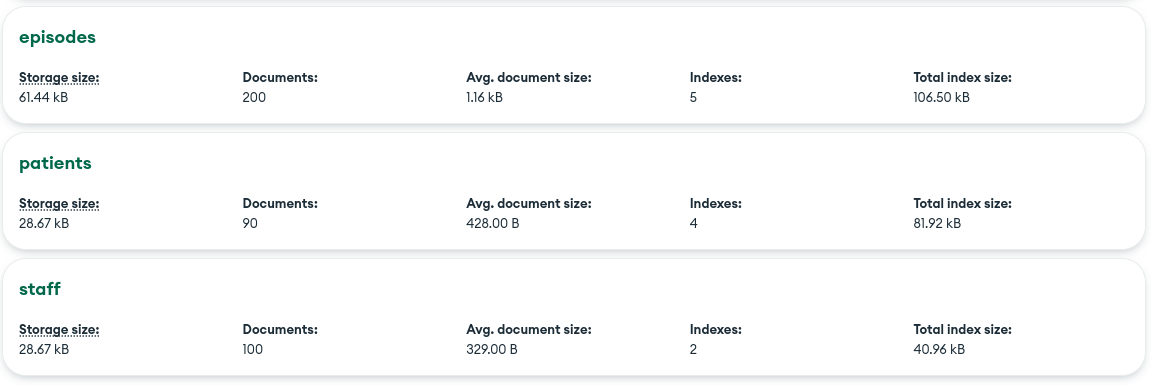
\includegraphics[width=0.9\linewidth]{Imagens/MongoDB/colecoes_mongo.png}
    \caption{Coleções criadas na base de dados MongoDB}
    \label{fig:colecoes_mongo}
\end{figure}

\section{Coleção Pacientes}
A coleção de Pacientes no MongoDB foi projetada para armazenar informações abrangentes sobre cada paciente, aproveitando a flexibilidade da estrutura de documentos JSON. Esta coleção inclui dados pessoais como nome, data de nascimento, tipo sanguíneo, contacto telefónico e e-mail. Além disso, armazena detalhes de seguros de saúde, contactos de emergência e histórico médico. No final um objeto paciente pertencente a esta coleção terá uma estrutura semelhante à seguinte:

\begin{myminted}{json}
{
  "_id": {"|\$|oid": "6658a65bf6d1a33ea5c68337"},
  "id_patient": 2,
  "patient_fname": "Jane",
  "patient_lname": "Smith",
  "blood_type": "O-",
  "phone": "987-654-3210",
  "email": "jane.smith@example.com",
  "gender": "Female",
  "birthday": {"|\$|date": "1990-03-20T00:00:00.000Z"},
  "insurance": {
    "policy_number": "POL002",
    "provider": "XYZ Insurance",
    "insurance_plan": "Premium Plan",
    "co_pay": 30,
    "coverage": "Partial Coverage",
    "maternity": false,
    "dental": true,
    "optical": true
  },
  "emergency_contact": [
    {
      "contact_name": "Jane Smith",
      "phone": "222-333-4444",
      "relation": "Mother"
    }
  ],
  "medical_history": [
    {
      "record_id": 2,
      "condition": "Allergy",
      "record_date": {"|\$|date": "2023-03-05T00:00:00.000Z"}
    }
  ]
}
\end{myminted}


\section{Coleção Staff}
A coleção de Staff no MongoDB foi desenvolvida para gerir de forma eficiente os dados relacionados aos funcionários do sistema de saúde, incluindo médicos, enfermeiros e técnicos. Esta coleção armazena informações detalhadas sobre cada funcionário, como nome, data de admissão, endereço, e-mail e número de segurança social. Também inclui detalhes específicos sobre o departamento ao qual pertencem, suas qualificações e o estado de atividade atual. Na base esta coleção faz uso da semelhança entre as tabelas de \textit{doctor}, \textit{nurse} e \textit{technician} agrupando-as com a tabela \textit{staff} e \textit{department}, utilizando o campo \textit{\textbf{role}} para identificação do funcionário de saúde em questão (\textit{DOCTOR}, \textit{NURSE}, \textit{TECHNICIAN}). O atributo \textit{\textbf{date\_of\_separation}} apenas se encontra presente nos funcionários que já abandonaram um determinado departamento, quando tal não acontece este campo não é acrescentado ao objeto JSON. Em seguida é apresentado um exemplo da estrutura implementada para o caso de um médico que ainda se mantém ativo no departamento em questão:

\begin{myminted}{json}
{
  "_id": {"|\$|oid": "6658a65bf6d1a33ea5c6838a"},
  "emp_id": 6,
  "emp_fname": "Lisa",
  "emp_lname": "Hayes",
  "date_joining": {"|\$|date": "2023-05-10T00:00:00.000Z"},
  "email": "mprice@example.com",
  "address": "Trevorfurt, IN 02637\"",
  "ssn": 685569160,
  "is_active_status": true,
  "department": {
    "id_department": 1,
    "department_head": "John Smith",
    "department_name": "Cardiology_1"
  },
  "role": "DOCTOR",
  "qualifications": "PhD"
}
\end{myminted}

\section{Coleção Episódios}

A coleção de Episódios no MongoDB foi criada para armazenar informações detalhadas sobre os episódios de atendimento dos pacientes, incluindo consultas, hospitalizações, prescrições, faturas e exames laboratoriais. Como esta coleção serve como uma ligação essencial entre as coleções de Pacientes e Staff, foi necessário encontrar uma maneira eficiente de traduzir essas relações. Uma das abordagens consideradas foi a criação de redundância nas coleções, aproveitando a flexibilidade do paradigma não relacional para replicar dados e adicionar informações úteis diretamente na coleção de Episódios. No entanto, para evitar a redundância excessiva, optou-se por utilizar identificadores de objetos de outras coleções, funcionando de maneira similar às chaves estrangeiras no paradigma relacional. Esta abordagem permite manter a integridade referencial e facilita consultas mais eficientes e organizadas, garantindo, assim, uma gestão mais eficaz dos dados. 

Para implementar esta abordagem, foi necessário armazenar em duas listas os IDs dos objetos de Pacientes e Staff que foram adicionados. Em Python, essa tarefa foi facilitada pelo uso da função \mintinline{python}{collection.insert_many()}. Esta função não apenas insere os elementos na coleção correspondente, mas também retorna um objeto contendo a lista de todos os IDs inseridos. Assim, antes de migrar os dados para a coleção de episódios, bastou obter duas listas contendo todos os IDs dos pacientes e membros do staff previamente inseridos. Com estas listas carregadas, foi possível estabelecer as relações necessárias entre as coleções de forma eficiente e precisa, garantindo que, por exemplo, cada episódio estivesse corretamente associado aos seus respetivos paciente e profissional de saúde. Se um indivíduo desta coleção fosse hospitalizado, recebesse prescrições de medicamentos e fosse submetido a exames médicos, a sua estrutura seria representada da seguinte forma na coleção:

\begin{myminted}{json}
{
  "_id": {"|\$|oid": "66603d8cc0c3dd4601195502"},
  "id_episode": 175,
  "id_patient": {"|\$|oid": "66603d8cc0c3dd460119543d"},
  "hospitalization": {
    "admission_date": {"|\$|date": "2020-11-03T00:00:00.000Z"},
    "discharge_date": {"|\$|date": "2020-11-04T00:00:00.000Z"},
    "responsible_nurse": {"|\$|oid": "66603d8cc0c3dd46011954ca"},
    "room": {
      "id_room": 40,
      "room_type": "Executive",
      "room_cost": 420
    }
  },
  "prescriptions": [
    {
      "id_prescription": 169,
      "prescription_date": {"|\$|date": "2020-11-03T00:00:00.000Z"},
      "dosage": 31,
      "medicine": {
        "id_medicine": 1,
        "m_name": "Paracetamol",
        "m_quantity": 50,
        "m_cost": 10
      }
    }
  ],
  "lab_screenings": [
    {
      "lab_id": 9,
      "test_cost": 93.19,
      "test_date": {"|\$|date": "2020-11-03T00:00:00.000Z"},
      "id_technician": {"|\$|oid": "66603d8cc0c3dd46011954f6"}
    }
  ]
}

\end{myminted}



\section{Triggers em MongoDB}
Durante o processo de migração de dados da base de dados Oracle para MongoDB, foi necessário definir diversos \textit{triggers} para otimizar a inserção de novos documentos e manter a integridade dos dados. Na nossa base de dados, procurávamos evitar o uso manual de campos de identificação durante a inserção de novos documentos preservando os campos de identificação originais, provenientes da base de dados Oracle, e mantendo a utilização de campos de identificação do mesmo tipo na base de dados MongoDB (além da utilização de identificadores do tipo ObjectId para o campo '\_id'). Para tal, utilizamos \textit{triggers} responsáveis por gerar automaticamente esses identificadores, garantindo a integridade e a unicidade dos dados.

Para alcançar este objetivo, optamos pela criação de uma coleção auxiliar denominada '\textit{counters}', responsável por armazenar o valor máximo de cada identificador inteiro existente, entre todos os valores já utilizados até ao momento. Cada documento desta coleção é utilizado para a geração do próximo valor de cada identificador único (similar às sequências em Oracle) durante a inserção de novos documentos ou substituição de documentos existentes nas restantes coleções da base de dados. Assim, na inserção de um novo documento, o contador correspondente, presente neste coleção '\textit{counters}', é incrementado, de modo obter o próximo valor do identificador, de acordo com a coleção na qual foi inserido um novo documento e o identificador em questão.

Além dos \textit{triggers} relacionados à criação de identificadores únicos, foi necessário adaptar um \textit{trigger} existente na base de dados original Oracle para o ambiente MongoDB. Este \textit{trigger} específico foi ajustado para garantir que sua funcionalidade fosse preservada após a migração, mantendo a consistência e a continuidade das operações automatizadas.

Em MongoDB, para a configuração e \textit{deployment} destes triggers, decidimos utilizar um \textit{cluster} criado na plataforma \textit{MongoDB Atlas}. Assim, de modo a automatizar a criação de triggers nesta plataforma, desenvolvemos diversos \textit{scripts} Python responsáveis pela criação, atualização, remoção e retoma (após uma falha no cluster, por exemplo) dos triggers na mesma, que utilizam pedidos \textit{HTTP} a APIs disponibilizadas pelo MongoDB de modo a efetuar as diversas operações descritas.


\subsection{Triggers para a adição de identificadores únicos}
Na sequencia da criação destes \textit{triggers} foi observada a existência de dois casos de geração de identificadores diferentes. Estes dois casos distintos dividiram a implementação em dois tipos principais: \textit{triggers} responsáveis pela geração de valores para os identificadores de cada documento e, \textit{triggers} responsáveis pela geração de valores para identificadores de objetos armazenados em listas/arrays presentes nos documentos das restantes coleções.

Assim sendo, para os campos 'id\_patient', 'id\_episode' e 'emp\_id', das coleções 'patients', 'episodes' e 'staff, respetivamente, foram criados três \textit{triggers} idênticos, acionados sempre que seja necessário gerar um novo identificador como valor de algum destes três campos, ou, caso o utilizador decida especificar o valor do identificador manualmente e possa, eventualmente, ser necessário atualizar o valor do contador correspondente ao campo em questão, para o valor do identificador inserido manualmente (caso este seja superior ao valor do contador). Deste modo, estes \textit{triggers} são executados apenas nos casos em que existe a inserção de um novo documento em qualquer uma das restantes coleções, sempre que um documento é substituído por um novo (\textit{replace)} e este último não apresenta identificador inteiro ou, o valor do identificador é alterado, através de uma operação de \textit{update} ou \textit{replace}, para um valor superior ao armazenado no contador corresponde e, portanto, é necessário atualizar o valor do contador. Para obter este comportamento e evitar que os \textit{triggers} fossem executados, por exemplo, quando são efetuados \textit{updates} a outros campos de cada documento, foi necessário definir uma expressão \texttt{\$match} no MongoDB Atlas.


Para o campo 'record\_id' existente nos objetos armazenados na lista 'medical\_history', presente nos documentos da coleção 'patients' e, para os campos 'id\_bill', 'id\_prescription' e 'lab\_id' existentes nos objetos armazenados nas listas 'bills', 'prescriptions' e 'lab\_screenings', respetivamente, da coleção 'episodes' foram criados quatro \textit{triggers} idênticos, acionados sempre que seja necessário gerar um novo identificador como valor de algum destes quatro campos, ou, caso o utilizador decida especificar o valor do identificador manualmente e possa, eventualmente, ser necessário atualizar o valor do contador correspondente ao campo em questão, para o valor do identificador inserido manualmente (caso este seja superior ao valor do contador). 

Deste modo, estes \textit{triggers} são executados apenas nos casos em que existe a inserção de um novo documento em qualquer uma das restantes coleções, sempre que um documento é substituído por um novo (\textit{replace)}, um novo objeto é inserido numa das listas referidas ou, o valor do identificador de um objeto é alterado, através de uma operação de \textit{update}. Tal como nos triggers anteriores, para obter este comportamento e evitar que os \textit{triggers} fossem executados, por exemplo, quando são efetuados \textit{updates} a outros campos de cada documento, foi necessário definir mais uma expressão \texttt{\$match} no MongoDB Atlas.


\subsection{Trigger proveniente da base de dados Oracle}

O \textit{trigger} proveniente da base de dados Oracle em questão têm como objetivo principal gerar automaticamente uma fatura (\textit{bill}) quando um paciente recebe uma alta hospitalar, ou seja, quando o campo \texttt{discharge\_date} é adicionado ao objeto '\texttt{hospitalization}' de um documento da coleção '\texttt{episodes}' com valor diferente de \texttt{null}, ou então, o seu valor é atualizado de \texttt{null} para um valor diferente de \texttt{null}. Assim sendo, este \textit{trigger} é, em primeiro lugar, apenas atualizado quando o documento em questão é atualizado (\texttt{update}) ou substituído (\texttt{replace}).
Para obter o comportamento e evitar que este \textit{trigger} fosse executado, por exemplo, quando são efetuados \textit{updates} a outros campos de cada documento, utilizamos a seguinte expressão de \texttt{\$match} no MongoDB Atlas, de modo a filtrar os casos em que não é pretendido gerar uma nova fatura.

\begin{myminted}{json}
{
    "fullDocumentBeforeChange.hospitalization.discharge_date": null,
    "fullDocument.hospitalization.discharge_date": {
        "|\$|ne": null
    }
}
\end{myminted}

Tal como em Oracle, este \textit{trigger} é responsável por monitorizar o valor do campo de alta hospitalar e, ao detetar uma atualização para um valor diferente de \texttt{null}, inicia uma série de processos para calcular os custos associados ao paciente durante sua estadia. Esses custos incluem taxas de quarto (\texttt{room\_cost}), custos de exames laboratoriais (\texttt{test\_cost}) e outros encargos médicos (\texttt{other\_charges}). A soma total desses custos resulta na criação de uma nova fatura, armazenada na lista \texttt{bills}. O código desenvolvido para a implementação deste \textit{trigger} é apresentado de seguida (a variável \texttt{service\_name} presente no código abaixo é substituído pelo nome do serviço do MongoDB Atlas).

\begin{myminted}{javascript}
function stringify(object) {
    return JSON.stringify(object).replaceAll('"', "'").replaceAll(':', ': ').replaceAll(',', ', ');
}

function isIterable(value) {
    return Symbol.iterator in Object(value);
}

exports = async function(changeEvent) {
    try {
        const fullDocument = changeEvent.fullDocument;
        const docId = changeEvent.documentKey._id;

        const serviceName = '{{ service_name }}';
        const databaseName = changeEvent.ns.db;
        const collectionName = changeEvent.ns.coll;

        const episodesCollection = context.services.get(serviceName).db(databaseName).collection(collectionName);

        // Calculate the room cost for the associated hospitalization
        let roomCost = 0;
        const hospitalization = fullDocument.hospitalization;
        
        if (hospitalization) {
          const room = hospitalization.room;
          
          if (room && room.room_cost) {
            roomCost = room.room_cost;
          }
        }
        
        // Calculate the test cost for the associated hospitalization
        let testsCost = 0;
        const lab_screenings = fullDocument.lab_screenings;
        
        if (isIterable(lab_screenings)) {
            for (test of lab_screenings) {
                if (test.test_cost) {
                    testsCost += test.test_cost;
                }
            }
        }
        
        // Calculate the other charges for prescriptions for the associated hospitalization
        let prescriptionsCost = 0;
        const prescriptions = fullDocument.prescriptions;
        
        if (isIterable(prescriptions)) {
            for (prescription of prescriptions) {
                const medicine = prescription.medicine;
                const dosage = prescription.dosage;
                
                if (medicine && dosage && medicine.m_cost) {
                    prescriptionsCost += medicine.m_cost * dosage; 
                }
            }
        }
        
        // Calculate the total cost of the bill for the associated episode
        const totalCost = roomCost + testsCost + prescriptionsCost;
        
        // Insert the bill with the total cost for the associated episode
        const newBill = {
          room_cost: roomCost,
          test_cost: testsCost,
          other_charges: prescriptionsCost,
          total: totalCost,
          registered_at: new Date(),
          payment_status: 'PENDING'
        }

        const billsListName = 'bills';
        const documentQuery = { _id: docId };

        await episodesCollection.updateOne(documentQuery, { |\$|push: { [billsListName]: newBill } });
        
        console.log(`Adicionada fatura ${stringify(newBill)} ao documento ${stringify(documentQuery)}, na lista '|\$|{billsListName}'.`);

    } catch (err) {
        console.error('Erro ao executar o trigger: ', err.message);
    }
};
\end{myminted}


Este \textit{trigger} garante que a transição do OracleDB para o MongoDB mantenha a mesma eficiência e precisão na criação de faturas, assegurando a continuidade das operações financeiras no ambiente hospitalar de uma forma otimizada.

\section{Scripts para gestão dos triggers no MongoDB Atlas}
Tal como referido, foram criados scripts \texttt{Python} responsáveis pela criação, atualização, remoção e retoma dos \textit{triggers} na plataforma MongoDB Atlas. Assim sendo, os quatros scripts desenvolvidos são apresentados na seguinte lista.

\begin{itemize}
    \item '\texttt{create\_triggers.py}' - Script responsável pela criação de \textit{triggers} na plataforma MongoDB Atlas. Os argumentos deste script são:
        \begin{itemize}
            \item '\texttt{-pubk}' ou '\texttt{--public-key}' - Chave pública da organização existente no MongoDB Atlas a utilizar;
            \item '\texttt{-privk}' ou '\texttt{--private-key}' - Chave privada da organização existente no MongoDB Atlas a utilizar;
            \item '\texttt{-pn}' ou '\texttt{--project-name}' - Nome do projeto MongoDB Atlas a utilizar;
            \item '\texttt{-cn}' ou '\texttt{--cluster-name}' - Nome do cluster MongoDB Atlas a utilizar;
            \item '\texttt{-f}' ou '\texttt{--file}' - Caminho para o ficheiro JSON de configuração dos triggers a utilizar;
        \end{itemize}
        
    \item '\texttt{update\_triggers.py}' - Script responsável pela atualização de \textit{triggers} já existentes na plataforma MongoDB Atlas. Os argumentos deste script são:
        \begin{itemize}
            \item '\texttt{-pubk}' ou '\texttt{--public-key}' - Chave pública da organização existente no MongoDB Atlas a utilizar;
            \item '\texttt{-privk}' ou '\texttt{--private-key}' - Chave privada da organização existente no MongoDB Atlas a utilizar;
            \item '\texttt{-pn}' ou '\texttt{--project-name}' - Nome do projeto MongoDB Atlas a utilizar;
            \item '\texttt{-cn}' ou '\texttt{--cluster-name}' - Nome do cluster MongoDB Atlas a utilizar;
            \item '\texttt{-f}' ou '\texttt{--file}' - Caminho para o ficheiro JSON de configuração dos triggers a utilizar;
        \end{itemize}
        
    \item '\texttt{delete\_triggers.py}' - Script responsável pela remoção de \textit{triggers} existentes na plataforma MongoDB Atlas. Os argumentos deste script são:
        \begin{itemize}
            \item '\texttt{-pubk}' ou '\texttt{--public-key}' - Chave pública da organização existente no MongoDB Atlas a utilizar;
            \item '\texttt{-privk}' ou '\texttt{--private-key}' - Chave privada da organização existente no MongoDB Atlas a utilizar;
            \item '\texttt{-pn}' ou '\texttt{--project-name}' - Nome do projeto MongoDB Atlas a utilizar;
            \item '\texttt{-f}' ou '\texttt{--file}' - Caminho para o ficheiro JSON de configuração dos triggers a utilizar;
        \end{itemize}
        
    \item '\texttt{delete\_triggers.py}' - Script responsável pela retoma (\textit{resume}) de \textit{triggers} suspensos na plataforma MongoDB Atlas. Os argumentos deste script são:
        \begin{itemize}
            \item '\texttt{-pubk}' ou '\texttt{--public-key}' - Chave pública da organização existente no MongoDB Atlas a utilizar;
            \item '\texttt{-privk}' ou '\texttt{--private-key}' - Chave privada da organização existente no MongoDB Atlas a utilizar;
            \item '\texttt{-pn}' ou '\texttt{--project-name}' - Nome do projeto MongoDB Atlas a utilizar;
            \item '\texttt{-f}' ou '\texttt{--file}' - Caminho para o ficheiro JSON de configuração dos triggers a utilizar;
        \end{itemize}
\end{itemize}

\section{Exploração da Base de Dados}
Após a migração para o MongoDB, conforme explicado anteriormente, iniciámos a exploração desta base de dados orientada a documentos. Para isso, usamos duas abordagens distintas. No primeiro caso, para consultar os dados concretos, isto é, passar por exemplo um ID de episódio foram usadas \textbf{funções}. Por outro lado, caso a consulta fosse com o objetivo de obter dados de maneira mais geral como o custo total dos exames laboratoriais e/ou o número total desses exames foram usadas \textbf{expressões}.

Para obter informações detalhadas de um episódio específico, utilizámos uma função simples que aceita um argumento, neste caso, o \textit{episodeId}. A função \texttt{getAllInfoByEpisodeId} foi implementada para buscar todos os documentos na coleção \textit{episodes} onde o campo \textit{id\_episode} coincide com o \textit{episodeId} fornecido. Abaixo encontra-se a implementação desta função:

\begin{myminted}{javascript}
function getAllInfoByEpisodeId(episodeId) {
    return db.episodes.find({
        id_episode: episodeId
    }).toArray();
}

getAllInfoByEpisodeId(89);
\end{myminted}

Esta função permite-nos recuperar rapidamente todas as informações associadas a um episódio específico, facilitando a análise detalhada e a verificação de dados individuais conforme necessário.

Outro exemplo seria:

\begin{myminted}{javascript}
function getPatientsByRoom(roomId) {
    return db.episodes.aggregate([
        {
            $match: { "hospitalization.room.id_room": roomId }
        },
        {
            $lookup: {
                from: "patients",
                localField: "id_patient",
                foreignField: "_id",
                as: "patient_info"
            }
        },
        {
            $unwind: "$patient_info"
        },
        {
            $project: {
                _id: 0,
                patient_id: "$patient_info._id",
                patient_fname: "$patient_info.patient_fname",
                patient_lname: "$patient_info.patient_lname",
                room: "$room"
            }
        }
    ]).toArray();
}
    
getPatientsByRoom(1)
\end{myminted}

Nesta expressão de agregação, utilizamos as seguintes etapas do pipeline de agregação:

\begin{itemize}
    \item \texttt{\$match}: Filtra os documentos da coleção \texttt{episodes} para incluir apenas aqueles onde o campo \texttt{hospitalization.room.id\_room} coincide com o \textit{roomId} fornecido.
    \item \texttt{\$lookup}: Faz uma junção (\textit{join}) com a coleção \texttt{patients} para obter informações adicionais sobre os pacientes, utilizando o campo \texttt{id\_patient} como referência.
    \item \texttt{\$unwind}: Decompõe o \textit{array} \texttt{patient\_info} para incluir as informações do paciente diretamente no documento.
    \item \texttt{\$project}: Reformata o resultado final para incluir apenas os campos desejados: \texttt{patient\_id}, \texttt{patient\_fname}, \texttt{patient\_lname} e \texttt{room}.
\end{itemize}

Esta função permite-nos obter uma lista detalhada de pacientes que estão internados num determinado quarto, proporcionando uma visão clara e organizada das informações dos pacientes.

Além disso, para obter \textit{insights} mais abrangentes e sumarizados sobre os dados, utilizámos expressões agregadas. Um exemplo disso é a agregação que calcula o custo total dos exames laboratoriais (\textit{lab\_screenings}) e o número total desses exames. A agregação é realizada com a seguinte expressão:

\begin{myminted}{javascript}
db.episodes.aggregate([
    { $unwind: "$lab_screenings" },
    { $group: {
        _id: null,
        totalCost: { $sum: "$lab_screenings.test_cost" },
        totalCount: { $sum: 1 }
    }},
    { $project: {
        _id: 0,
        totalCost: 1,
        totalCount: 1
    }}
])
\end{myminted}

Nesta expressão, utilizamos várias etapas do pipeline de agregação: o \texttt{\$unwind} decompõe o \textit{array} \texttt{lab\_screenings} em múltiplos documentos, cada um contendo um único elemento do \textit{array}; o \texttt{\$group} agrupa todos os documentos, somando os custos dos exames e contando o número total de exames; e o \texttt{\$project} reformata o resultado para exibir apenas os campos \texttt{totalCost} e \texttt{totalCount}.

Outro exemplo seria:

\begin{myminted}{javascript}
db.episodes.aggregate([
        {
            $unwind: "$appointment"
        },
        {
            $group: {
                _id: "$appointment.id_doctor",
                totalAppointments: { $sum: 1 }
            }
        },
        {
            $sort: { totalAppointments: -1 }
        },
        {
            $lookup: {
                from: "staff",
                localField: "_id",
                foreignField: "_id",
                as: "doctor_info"
            }
        },
        {
            $unwind: "$doctor_info"
        },
        {
            $lookup: {
                from: "episodes",
                localField: "_id",
                foreignField: "appointment.id_doctor",
                as: "appointments"
            }
        },
        {
            $project: {
                _id: 0,
                doctor_id: "$_id",
                doctor_fname: "$doctor_info.emp_fname",
                doctor_lname: "$doctor_info.emp_lname",
                doctor_email: "$doctor_info.email",
                totalAppointments: 1,
            }
        }
    ])
\end{myminted}

Nesta expressão de agregação, utilizamos as seguintes etapas do pipeline de agregação:

\begin{itemize}
    \item \texttt{\$unwind}: Esta etapa decompõe o \textit{array} \texttt{appointment} em múltiplos documentos, cada um contendo um único elemento do \textit{array}.
    \item \texttt{\$group}: Agrupa os documentos pelo campo \texttt{id\_doctor} dentro de \texttt{appointment}, contando o número total de consultas (\texttt{totalAppointments}) para cada médico.
    \item \texttt{\$sort}: Ordena os resultados pelo número total de consultas em ordem decrescente.
    \item \texttt{\$lookup}: Faz uma junção (\textit{join}) com a coleção \texttt{staff} para obter informações adicionais sobre o médico, utilizando o campo \texttt{\_id} como referência.
    \item \texttt{\$unwind}: Decompõe o \textit{array} \texttt{doctor\_info} para incluir as informações do médico diretamente no documento.
    \item \texttt{\$lookup}: Faz outra junção (\textit{join}) com a coleção \texttt{episodes} para obter todas as consultas relacionadas ao médico específico.
    \item \texttt{\$project}: Reformata o resultado final para incluir apenas os campos desejados: \texttt{doctor\_id}, \texttt{doctor\_fname}, \texttt{doctor\_lname}, \texttt{doctor\_email} e \texttt{totalAppointments}.
\end{itemize}

É importante mencionar que a utilização de uma base de dados orientada a documentos, como o MongoDB, oferece várias vantagens para o bom desempenho da \textit{expressão} fornecida. As vantagens do MongoDB para a execução da expressão fornecida são várias, especialmente no contexto da agregação de dados e das funcionalidades específicas que o MongoDB oferece. Vamos detalhar algumas dessas vantagens:

\begin{enumerate}
    \item \textbf{Modelo de Dados Flexível:} MongoDB utiliza um modelo de dados baseado em documentos, que permite a representação de dados complexos e hierárquicos de forma mais natural e eficiente. No caso desta expressão, a capacidade de armazenar arrays e subdocumentos permite a estruturação dos dados de uma maneira que simplifica o processo de agregação.
    \item \textbf{Pipeline de Agregação Poderosa:} A framework de agregação do MongoDB oferece um pipeline poderosa e flexível para processar e transformar dados. A expressão fornecida utiliza várias etapas do pipeline de agregação, como \$unwind, \$group, \$sort, \$lookup e \$project, cada uma desempenhando uma função específica e eficiente no processamento dos dados.
    \item \textbf{Desempenho e Escalabilidade:} MongoDB é projetado para ser escalável horizontalmente, o que significa que pode lidar com grandes volumes de dados e consultas complexas de maneira eficiente. A indexação adequada pode otimizar ainda mais a performance das consultas, especialmente aquelas que envolvem operações de agregação complexas.
\end{enumerate}

Estas ferramentas e técnicas são essenciais para a exploração eficiente de bases de dados no MongoDB, permitindo-nos manipular grandes volumes de dados e extrair informações relevantes de maneira rápida e eficaz.

\subsection{Operações Básicas em MongoDB}

Numa base de dados NoSQL como o MongoDB, não é necessário implementar funções separadas para realizar operações básicas como inserir, apagar ou atualizar documentos. O MongoDB fornece métodos internos para lidar diretamente com estas operações. Aqui está um breve resumo de como pode realizar estas operações no MongoDB:

\begin{itemize}
    \item \textbf{Inserir Documentos:} Para inserir um documento numa coleção, pode usar os métodos \texttt{insertOne} ou \texttt{insertMany}.
    \item \textbf{Apagar Documentos:} Para apagar documentos, pode usar os métodos \texttt{deleteOne} ou \texttt{deleteMany}.
    \item \textbf{Atualizar Documentos:} Para atualizar documentos, pode usar os métodos \texttt{updateOne}, \texttt{updateMany} ou \texttt{replaceOne}.
\end{itemize}

O MongoDB, sendo uma base de dados NoSQL, é projetado para manipular dados de forma mais flexível e direta, eliminando a necessidade de mecanismos de controlo adicionais nas operações de \textbf{Criação} (\textit{CREATE}), \textbf{Atualização} (\textit{UPDATE}) e \textbf{Remoção} (\textit{DELETE}). 

De seguida, iremos apresentar e explicar de forma breve cada uma das funções e expressões implementadas.

%-> Um paragrafo a mencionar que, devido a mecanismos do MongoDB para inserção, ataulização e remoção da BD não foi necessário realizar a sua implementação, ao contrário do Oracle SQL. (mencionar a natureza NoSQL), mencionar que não é necessário estes mecanismos de controlo nas operações CUD (CREATE, UPDATE, DELETE)

\subsection{Visão Paciente}
\subsubsection{Funções}

\vspace{0.15cm}

\textbf{getPatientById}: Obtém informações de um paciente específico, dado um \textit{id\_patient}. Recebe ID como argumento e retorna os dados do paciente.

\vspace{0.15cm}

\textbf{getMedicalHistoryById}: Obtém o histórico médico de um paciente específico. Recebe ID como argumento e retorna todo o histórico médico do paciente.

\vspace{0.15cm}

\textbf{getInsuranceById}: Obtém as informações de seguro de um paciente específico. Recebe ID como argumento e retorna os dados do seguro do paciente.

\vspace{0.15cm}

\textbf{getEmergencyContactById}: Obtém o contacto de emergência de um paciente específico. Recebe ID como argumento e retorna os dados do contacto de emergência.

\vspace{0.15cm}

\textbf{getPatientsByBloodType}: Obtém pacientes por tipo sanguíneo. Recebe \textit{bloodType} como argumento e retorna os pacientes com o tipo sanguíneo especificado.

\vspace{0.15cm}

\textbf{getPatientsByGender}: Obtém pacientes por género. Recebe \textit{gender} como argumento e retorna os pacientes com o género especificado.

\vspace{0.15cm}

\textbf{getPatientsByCondition}: Obtém pacientes por condição médica. Recebe \textit{condition} como argumento e retorna os pacientes com a condição médica especificada.

\vspace{0.15cm}

\textbf{getPatientsByMedicalRecordDate}: Obtém pacientes com registros médicos em uma data específica. Recebe \textit{date} como argumento e retorna os pacientes com registos nessa data.

\vspace{0.15cm}

\textbf{countStaffByRole}: Conta o número de enfermeiros, doutores e técnicos. Retorna um objeto com as contagens de cada papel.

\vspace{0.15cm}

\textbf{getPatientsByMedicalRecordDateRange}: Obtém pacientes com registros médicos em um intervalo de datas. Recebe \textit{startDate} e \textit{endDate} como argumentos e retorna os pacientes com registos nesse intervalo.

\vspace{0.15cm}

\textbf{getPatientsByBirthday}: Obtém pacientes com uma data de aniversário específica. Recebe \textit{birthday} como argumento e retorna os pacientes com essa data de aniversário.

\vspace{0.15cm}

\textbf{getPatientsByInsuranceProvider}: Obtém pacientes por provedor de seguro. Recebe \textit{provider} como argumento e retorna os pacientes com o provedor de seguro especificado.

\vspace{0.15cm}

\textbf{getPatientsByInsurancePlan}: Obtém pacientes por plano de seguro. Recebe \textit{plan} como argumento e retorna os pacientes com o plano de seguro especificado.

\vspace{0.15cm}

\textbf{getPatientsByCoverage}: Obtém pacientes por tipo de cobertura. Recebe \textit{coverage} como argumento e retorna os pacientes com o tipo de cobertura especificado.

\vspace{0.15cm}

\textbf{listPatientsByAgeRange}: Lista pacientes por intervalo de idades. Recebe \textit{minAge} e \textit{maxAge} como argumentos e retorna os pacientes dentro desse intervalo de idades.

\vspace{0.15cm}

\textbf{listPatientsWithMaternityCoverage}: Obtém pacientes com cobertura de maternidade. Recebe boolean \textit{maternity} como argumento e retorna os pacientes com cobertura de maternidade.

\vspace{0.15cm}

\textbf{listPatientsWithDentalCoverage}: Obtém pacientes com cobertura dental. Recebe boolean \textit{dental} como argumento e retorna os pacientes com cobertura dental.

\vspace{0.15cm}

\textbf{listPatientsWithOpticalCoverage}: Obtém pacientes com cobertura ótica. Recebe boolean \textit{optical} como argumento e retorna os pacientes com cobertura ótica.

\vspace{0.15cm}

\textbf{findPatientsByEmergencyContactRelation}: Obtém pacientes por relação de contacto de emergência. Recebe \textit{relation} como argumento e retorna os pacientes com essa relação de contacto.

\vspace{0.15cm}

\textbf{getPatientByName}: Obtém um paciente pelo primeiro nome e sobrenome. Recebe \textit{firstName} e \textit{lastName} como argumentos e retorna o paciente com os nomes especificados.

\vspace{0.15cm}

\textbf{getPatientByPhone}: Obtém um paciente pelo número de telefone. Recebe \textit{phone} como argumento e retorna o paciente com o número de telefone especificado.

\vspace{0.15cm}

\textbf{getPatientsByEmergencyContact}: Obtém pacientes com um contacto de emergência específico. Recebe \textit{firstName} e \textit{lastName} como argumentos e retorna os pacientes com o contacto de emergência especificado.

\vspace{0.15cm}

\textbf{getPatientsByRecordId}: Obtém pacientes pelo \textit{record\_id} do histórico médico. Recebe \textit{recordId} como argumento e retorna os pacientes com o \textit{record\_id} especificado.

\vspace{0.15cm}

\textbf{getEpisodesByCondition}: Obtém episódios médicos por condição médica. Recebe \textit{condition} como argumento e retorna os episódios médicos com a condição especificada.

\vspace{0.3cm}

\subsubsection{Expressões}

\vspace{0.15cm}

\textbf{Buscar Todos os Tipos de Relações em Contactos de Emergência}: Obtém todos os tipos de relações em contactos de emergência. Desagrupa os contactos de emergência e agrupa por tipo de relação, retornando os tipos de relação.

\vspace{0.15cm}

\textbf{Buscar Todos os Tipos de Provedores de Seguro}: Obtém todos os tipos de provedores de seguro. Agrupa por provedores de seguro, retornando os tipos de provedores.

\vspace{0.15cm}

\textbf{Buscar Todos os Tipos de Planos de Seguro}: Obtém todos os tipos de planos de seguro. Agrupa por planos de seguro, retornando os tipos de planos.

\vspace{0.15cm}

\textbf{Buscar Todos os Tipos de Coverage}: Obtém todos os tipos de cobertura de seguro. Agrupa por tipos de cobertura, retornando os tipos de cobertura.

\vspace{0.15cm}

\textbf{Buscar Todos os Tipos de Condições Médicas}: Obtém todos os tipos de condições médicas. Desagrupa o histórico médico e agrupa por condição médica, retornando os tipos de condições.

\vspace{0.15cm}

\textbf{Buscar Todos os Tipos Sanguíneos}: Obtém todos os tipos sanguíneos. Agrupa por tipo sanguíneo, retornando os tipos sanguíneos.

\vspace{0.15cm}

\textbf{Buscar quantos Pacientes existem para cada BloodType}: Conta o número de pacientes para cada tipo sanguíneo. Agrupa por tipo sanguíneo e retorna a contagem de pacientes para cada tipo.

\vspace{0.15cm}

\textbf{Buscar quantos Pacientes existem para cada Condition}: Conta o número de pacientes para cada condição médica. Desagrupa o histórico médico e agrupa por condição médica, retornando a contagem de pacientes para cada condição.

\subsection{Visão Staff}
\subsubsection{Funções}

\vspace{0.15cm}

\textbf{getStaffInfo}: Obtém todas as informações de um membro do staff, dado um \textit{emp\_id}. Recebe \textit{emp\_id} como argumento e retorna os dados do membro do staff.

\vspace{0.15cm}

\textbf{getDepartmentInfo}: Obtém as informações do departamento de um membro do staff para um dado \textit{emp\_id}. Recebe \textit{emp\_id} como argumento e retorna os dados do departamento ou \textit{null} se não houver.

\vspace{0.15cm}

\textbf{AllInfoStaffByDateJoining}: Obtém todas as informações dos membros do staff que se juntaram em uma data específica. Recebe \textit{date\_joining} como argumento e retorna os dados dos membros do staff.

\vspace{0.15cm}

\textbf{AllInfoStaffByDateSeparation}: Obtém todas as informações dos membros do staff que se separaram em uma data específica. Recebe \textit{date\_separation\_str} como argumento e retorna os dados dos membros do staff.

\vspace{0.15cm}

\textbf{getStaffByActiveStatus}: Obtém todos os membros do staff com um status de atividade específico. Recebe \textit{is\_active\_status} como argumento e retorna os dados dos membros do staff.

\vspace{0.15cm}

\textbf{getQualificationsByDoctor}: Obtém as qualificações de um doutor específico. Recebe \textit{emp\_id} como argumento e retorna as qualificações do doutor ou \textit{null} se não houver.

\vspace{0.15cm}

\textbf{getStaffByName}: Obtém um membro do staff pelo primeiro nome e sobrenome. Recebe \textit{firstName} e \textit{lastName} como argumentos e retorna os dados do membro do staff.

\vspace{0.15cm}

\textbf{getStaffByEmail}: Obtém um membro do staff pelo email. Recebe \textit{email} como argumento e retorna os dados do membro do staff.

\vspace{0.15cm}

\textbf{getStaffBySSN}: Obtém um membro do staff pelo (\textit{SSN}). Recebe \textit{ssn} como argumento e retorna os dados do membro do staff.

\subsubsection{Expressões}

\textbf{Buscar toda a informação das Enfermeiras}: Obtém todas as informações dos membros do staff que têm o papel de \textit{NURSE}. Retorna uma lista com os dados das enfermeiras.

\vspace{0.15cm}

\textbf{Buscar toda a informação dos Médicos}: Obtém todas as informações dos membros do staff que têm o papel de \textit{DOCTOR}. Retorna uma lista com os dados dos médicos.

\vspace{0.15cm}

\textbf{Buscar toda a informação dos Técnicos}: Obtém todas as informações dos membros do staff que têm o papel de \textit{TECHNICIAN}. Retorna uma lista com os dados dos técnicos.

\vspace{0.15cm}

\textbf{Buscar quantos Enfermeiros existem}: Conta o número de membros do staff com o papel de \textit{NURSE}. Retorna a contagem de enfermeiros.

\vspace{0.15cm}

\textbf{Buscar quantos Doutores existem}: Conta o número de membros do staff com o papel de \textit{DOCTOR}. Retorna a contagem de doutores.

\vspace{0.15cm}

\textbf{Buscar quantos Técnicos existem}: Conta o número de membros do staff com o papel de \textit{TECHNICIAN}. Retorna a contagem de técnicos.

\vspace{0.15cm}

\textbf{Buscar quantos Departments existem}: Conta o número de departamentos diferentes. Agrupa por \textit{id\_department} e retorna a contagem de departamentos.

\vspace{0.15cm}

\textbf{Buscar todos os tipos de Qualifications}: Obtém todos os tipos de qualificações dos doutores. Desagrupa as qualificações e agrupa por tipo de qualificação, retornando os tipos de qualificações.

\vspace{0.15cm}

\textbf{Número de Empregados por Departamento}: Conta o número de empregados por departamento. Agrupa por \textit{id\_department} e retorna a contagem de empregados para cada departamento.

\vspace{0.15cm}

\textbf{Nurses por Departamento}: Conta o número de enfermeiras por departamento. Agrupa por \textit{id\_department} e retorna a contagem de enfermeiras para cada departamento.

\vspace{0.15cm}

\textbf{Número de Doctors por Departamento}: Conta o número de doutores por departamento. Agrupa por \textit{id\_department} e retorna a contagem de doutores para cada departamento.

\vspace{0.15cm}

\textbf{Número de Technicians por Departamento}: Conta o número de técnicos por departamento. Agrupa por \textit{id\_department} e retorna a contagem de técnicos para cada departamento.

\vspace{0.15cm}

\textbf{Contar o Número Total de Staff}: Conta o número total de membros do staff. Retorna a contagem total de membros.

\vspace{0.15cm}

\textbf{Buscar todos os Staff que Estão Ativos}: Obtém todos os membros do staff que estão ativos. Retorna uma lista com os dados dos membros ativos.

\vspace{0.15cm}

\textbf{Buscar todos os Staff que não estão Ativos}: Obtém todos os membros do staff que não estão ativos. Retorna uma lista com os dados dos membros inativos.

\vspace{0.15cm}

\textbf{Contar quantos Staff Estão Ativos}: Conta o número de membros do staff que estão ativos. Retorna a contagem de membros ativos.

\vspace{0.15cm}

\textbf{Contar quantos Staff não estão Ativos}: Conta o número de membros do staff que não estão ativos. Retorna a contagem de membros inativos.

\subsection{Visão Episodes}

\subsubsection{Funções}

\vspace{0.15cm}

\textbf{getAllInfoByEpisodeId}: Esta função retorna todas as informações sobre um episódio específico, dado um \texttt{episodeId}. Recebe um \texttt{episodeId} como argumento e retorna todos os documentos que correspondem a esse ID na coleção \texttt{episodes}.

\vspace{0.15cm}

\textbf{getAllInfoByEpisodeId\_withNames}: Retorna todas as informações sobre um episódio específico, incluindo informações do paciente, dado um \texttt{episodeId}. Recebe um \texttt{episodeId} e retorna documentos agregados com detalhes do paciente.

\vspace{0.15cm}

\textbf{getAllInfoByPrescriptionId}: Retorna todas as informações sobre uma prescrição específica dentro dos episódios. Recebe um \texttt{prescriptionId} e retorna os documentos que contêm essa prescrição.

\vspace{0.15cm}

\textbf{getPrescriptionById}: Obtém detalhes específicos de uma prescrição. Recebe um \texttt{prescriptionId} e retorna os detalhes da prescrição sem outros dados do episódio.

\vspace{0.15cm}

\textbf{getAllInfoByPatientId}: Retorna todas as informações sobre os episódios de um paciente específico. Recebe um \texttt{id\_patient} e retorna os episódios desse paciente.

\vspace{0.15cm}

\textbf{getPatientEpisodes}: Conta o número de episódios para um paciente específico. Recebe um \texttt{id\_patient} e retorna a contagem de episódios.

\vspace{0.15cm}

\textbf{getPrescriptionsByEpisodeId}: Obtém todas as prescrições de um episódio específico. Recebe um \texttt{episodeId} e retorna as prescrições desse episódio.

\vspace{0.15cm}

\textbf{getBillsByEpisodeId}: Retorna todas as faturas de um episódio específico. Recebe um \texttt{episodeId} e retorna as faturas desse episódio.

\vspace{0.15cm}

\textbf{getBillById}: Obtém uma fatura específica por \texttt{id\_bill}. Recebe um \texttt{id\_bill} e retorna a fatura correspondente.

\vspace{0.15cm}

\textbf{getLabScreeningsByEpisodeId}: Retorna todos os exames laboratoriais de um episódio específico. Recebe um \texttt{episodeId} e retorna os exames laboratoriais desse episódio.

\vspace{0.15cm}

\textbf{getHospitalizationByEpisodeId}: Obtém informações de hospitalização para um episódio específico. Recebe um \texttt{episodeId} e projeta apenas o campo \texttt{hospitalization} no resultado.

\vspace{0.15cm}

\textbf{getRoomById}: Obtém informações de uma sala específica com base no seu ID. Recebe \texttt{roomId} como argumento e retorna os dados da sala correspondente.

\vspace{0.15cm}

\textbf{getPrescriptionsByPatientId}: Obtém todas as prescrições associadas a um paciente específico. Recebe \texttt{patientId} como argumento e retorna uma lista de prescrições desse paciente.

\vspace{0.15cm}

\textbf{getBillsByPatientId}: Obtém todas as faturas relacionadas a um paciente. Recebe \texttt{patientId} como argumento e retorna as faturas correspondentes.

\vspace{0.15cm}

\textbf{getLabScreeningsByPatientId}: Obtém todos os exames laboratoriais de um paciente. Recebe \texttt{patientId} como argumento e retorna os exames laboratoriais desse paciente.

\vspace{0.15cm}

\textbf{getHospitalizationByPatientId}: Obtém informações de hospitalização para um paciente específico. Recebe \texttt{patientId} como argumento e retorna os dados de hospitalização.

\vspace{0.15cm}

\textbf{getRoomsByPatientId}: Obtém todas as salas associadas às hospitalizações de um paciente. Recebe \texttt{patientId} como argumento e retorna os dados das salas.

\vspace{0.15cm}

\textbf{getMedicinesByPatientId}: Obtém todas as informações de medicamentos prescritos para um paciente. Recebe \texttt{patientId} como argumento e retorna os dados dos medicamentos.

\vspace{0.15cm}

\textbf{getMedicinesByEpisodeId}: Obtém todos os medicamentos prescritos em um episódio específico. Recebe \texttt{episodeId} como argumento e retorna os dados dos medicamentos desse episódio.

\vspace{0.15cm}

\textbf{getMedicineById}: Obtém os dados de um medicamento específico. Recebe \texttt{medicineId} como argumento e retorna os dados do medicamento.

\vspace{0.15cm}

\textbf{getMedicineByPrescriptionId}: Obtém informações dos medicamentos associados a uma prescrição específica. Recebe \texttt{prescriptionId} como argumento e retorna os dados dos medicamentos dessa prescrição.

\vspace{0.15cm}

\textbf{getMedicineByName}: Esta função obtém informações de um medicamento específico pelo seu nome. Recebe \textit{medicineName} como argumento e retorna os dados do medicamento.

\vspace{0.15cm}

\textbf{getPrescriptionsByDate}: Obtém todas as prescrições em uma data específica. Recebe \textit{date} como argumento e retorna as prescrições dessa data.

\vspace{0.15cm}

\textbf{getPrescriptionsBetweenDates}: Obtém todas as prescrições entre duas datas. Recebe \textit{startDate} e \textit{endDate} como argumentos e retorna as prescrições nesse intervalo de datas.

\vspace{0.15cm}

\textbf{getPrescriptionsBetweenDosages}: Obtém todas as prescrições entre duas dosagens. Recebe \textit{minDosage} e \textit{maxDosage} como argumentos e retorna as prescrições dentro desse intervalo de dosagens.

\vspace{0.15cm}

\textbf{getTotalBillsByPatientId}: Soma o total das faturas para um paciente específico. Recebe \textit{patientId} como argumento e retorna o valor total das faturas.

\vspace{0.15cm}

\textbf{getTotalCostsByPatientId}: Soma todas as contas (room cost, test cost, e other charges) para um paciente específico. Recebe \textit{patientId} como argumento e retorna os custos totais.

\vspace{0.15cm}

\textbf{getLabScreeningsByDateRange}: Obtém todos os exames laboratoriais dentro de um intervalo de datas. Recebe \textit{startDate} e \textit{endDate} como argumentos e retorna os exames laboratoriais nesse intervalo.

\vspace{0.15cm}

\textbf{getLabScreeningsByPriceRange}: Obtém todos os exames laboratoriais dentro de um intervalo de custo. Recebe \textit{minPrice} e \textit{maxPrice} como argumentos e retorna os exames laboratoriais dentro desse intervalo de custo.

\vspace{0.15cm}

\textbf{getHospitalizationsByDateRange}: Obtém registros de hospitalização com base em um intervalo de datas de admissão e alta. Recebe \textit{startDate} e \textit{endDate} como argumentos e retorna as hospitalizações nesse intervalo de datas.

\vspace{0.15cm}

\textbf{getAppointmentsByPatientId}: Obtém todas as consultas de um paciente específico. Recebe \textit{patientId} como argumento e retorna as consultas desse paciente.

\vspace{0.15cm}

\textbf{getAppointmentsByPatientId}: Obtém todas as consultas de um paciente específico. Recebe \textit{patientId} como argumento e retorna as consultas desse paciente.

\vspace{0.15cm}

\textbf{getAppointmentsByEpisodeId}: Obtém todas as consultas de um episódio específico. Recebe \textit{episodeId} como argumento e retorna as consultas desse episódio.

\vspace{0.15cm}

\textbf{getAppointmentsByScheduleOnDate}: Obtém todas as consultas agendadas para uma data específica. Recebe \textit{date} como argumento e retorna as consultas agendadas nessa data.

\vspace{0.15cm}

\textbf{getAppointmentsByAppointmentDate}: Obtém todas as consultas para uma data específica. Recebe \textit{date} como argumento e retorna as consultas dessa data.

\vspace{0.15cm}

\textbf{getAppointmentsByAppointmentTime}: Obtém todas as consultas para um horário específico. Recebe \textit{time} como argumento e retorna as consultas desse horário.

\vspace{0.15cm}

\textbf{getAppointmentsByDoctorId}: Obtém todas as consultas de um médico específico. Recebe \textit{doctorId} como argumento e retorna as consultas desse médico.

\vspace{0.15cm}

\textbf{getBillsByDateRange}: Obtém todas as faturas registradas entre duas datas específicas. Recebe \textit{startDate} e \textit{endDate} como argumentos e retorna as faturas registradas nesse intervalo de datas.

\vspace{0.15cm}

\textbf{getPatientsByPaymentStatus}: Obtém pacientes com um \textit{payment\_status} específico. Recebe \textit{status} como argumento e retorna os dados dos pacientes e seus episódios com o status de pagamento especificado.

\vspace{0.15cm}

\textbf{getTotalCostByRegisteredDate}: Calcula o custo total das faturas registradas entre duas datas. Recebe \textit{startDate} e \textit{endDate} como argumentos e retorna o custo total das faturas nesse intervalo de datas.

\vspace{0.15cm}

\textbf{getNurseInfoByEpisodeId}: Obtém informações da enfermeira responsável por um episódio específico. Recebe \textit{episodeId} como argumento e retorna os dados da enfermeira responsável.

\vspace{0.15cm}

\textbf{getNursesByPatientId}: Obtém todas as enfermeiras que já cuidaram de um determinado paciente. Recebe \textit{patientId} como argumento e retorna os dados das enfermeiras.

\vspace{0.15cm}

\textbf{getDoctorInfoByEpisodeId}: Obtém informações do médico responsável por um episódio específico. Recebe \textit{episodeId} como argumento e retorna os dados do médico responsável.

\vspace{0.15cm}

\textbf{getDoctorsByPatientId}: Obtém todas as informações dos médicos que atenderam um paciente específico. Recebe \textit{patientId} como argumento e retorna os dados dos médicos.

\vspace{0.15cm}

\textbf{getTechnicianInfoByEpisodeId}: Obtém informações do técnico responsável por um episódio específico. Recebe \textit{episodeId} como argumento e retorna os dados do técnico responsável.

\vspace{0.15cm}

\textbf{getTechniciansByPatientId}: Obtém todas as informações dos técnicos que atenderam um paciente específico. Recebe \textit{patientId} como argumento e retorna os dados dos técnicos.

\vspace{0.15cm}

\textbf{getPatientInfoByIdFromEpisodes}: Retorna informações de um paciente específico, dado um \textit{id\_patient}. Recebe \textit{patientId} como argumento e retorna os dados do paciente.

\vspace{0.15cm}

\textbf{getPatientsByRoom}: Lista os pacientes alocados a um quarto específico. Recebe \textit{roomId} como argumento e retorna os dados dos pacientes e informações do quarto.

\vspace{0.15cm}

\textbf{getHospitalizationsByNurse}: Lista hospitalizações por enfermeira responsável. Recebe \textit{nurseId} como argumento e retorna os dados das hospitalizações e da enfermeira.

\vspace{0.15cm}

\textbf{getAllEpisodesForPatient}: Lista todos os episódios médicos de um paciente específico. Recebe \textit{patientId} como argumento e retorna os episódios do paciente.

\vspace{0.15cm}

\textbf{getEpisodesByDoctor}: Lista todos os episódios médicos de um médico específico. Recebe \textit{doctorId} como argumento e retorna os episódios do médico.

\vspace{0.15cm}

\textbf{getLabScreeningsByTechnician}: Lista exames baseados no técnico responsável. Recebe \textit{technicianId} como argumento e retorna os exames e informações do técnico.

\vspace{0.15cm}

\textbf{getAppointmentsByDateAndTime}: Busca consultas por data e horário específico. Recebe \textit{date} e \textit{time} como argumentos e retorna as consultas e informações dos pacientes.

\vspace{0.15cm}

\textbf{getAppointmentsByDoctorByDay}: Lista as consultas de um médico específico por dia. Recebe \textit{doctorId} como argumento e retorna as consultas agrupadas por dia, com detalhes dos pacientes e do médico.

\subsubsection{Expressões}

\vspace{0.15cm}

\textbf{Contar \textit{Appointments} por Médico}: Conta o número total de consultas para cada médico. Agrupa os resultados pelo campo \texttt{id\_doctor} e retorna o número total de consultas para cada médico.

\vspace{0.15cm}

\textbf{Calcular o Total de Medicamentos e Custo Total}: Calcula o total de medicamentos e o custo total de todos os medicamentos prescritos. Agrupa os resultados e retorna a quantidade total e o custo total.

\vspace{0.15cm}

\textbf{Calcular o Total de Cada Medicamento Usado e o Custo Total}: Calcula a quantidade total e o custo total para cada tipo de medicamento usado. Agrupa os resultados pelo nome do medicamento e retorna a quantidade total e o custo total para cada medicamento.

\vspace{0.15cm}

\textbf{Calcular o Custo Total dos Testes e a Contagem de Testes Realizados}: Calcula o custo total dos testes e a contagem de testes realizados. Agrupa os resultados e retorna o custo total e o número total de testes.

\vspace{0.15cm}

\textbf{Buscar Todas as Faturas com Detalhes dos Pacientes}: Obtém todas as faturas com detalhes dos pacientes associados. Realiza uma junção com a coleção \texttt{patients} para incluir informações dos pacientes.

\vspace{0.15cm}

\textbf{Buscar Todos os Episódios que Ainda Não Acabaram}: Obtém todos os episódios que ainda não foram encerrados. Retorna os episódios com a data de alta nula.

\vspace{0.15cm}

\textbf{Buscar Informações de Todos os Pacientes}: Obtém informações de todos os pacientes associados aos episódios. Retorna os dados agregados dos pacientes.

\vspace{0.15cm}

\textbf{Buscar Todos os Episódios e o Respetivo Paciente}: Obtém todos os episódios e os dados do paciente associado. Retorna as informações dos episódios e dos pacientes.

\vspace{0.15cm}

\textbf{Lista os Médicos com Mais Consultas Marcadas}: Lista os médicos com mais consultas marcadas. Agrupa e ordena os médicos pelo número total de consultas, retornando os dados dos médicos e o total de consultas.

\vspace{0.15cm}

\textbf{Lista os Médicos com Mais Consultas Marcadas, com Informação Detalhada do Paciente}: Lista os médicos com mais consultas marcadas, incluindo detalhes dos pacientes. Agrupa e ordena os médicos pelo número total de consultas, retornando os dados dos médicos e informações detalhadas dos pacientes.
\chapter{Base de dados orientada a grafos - Neo4J}
\paragraph{}
Além da migração para uma base de dados não relacional orientada a documentos, também implementamos um modelo na base de dados \textbf{Neo4j}, conhecida por sua orientação a grafos. Após uma análise aprofundada do nosso esquema relacional inicial, identificamos as relações mais significativas que podem ser representadas de forma eficiente neste paradigma não relacional.

O Neo4j permite a modelagem de dados em termos de nós e relacionamentos, proporcionando uma representação intuitiva das interconexões entre os dados. Com base nessa abordagem, identificamos e selecionamos os nós mais relevantes para representar corretamente as informações no Neo4j. Além disso, escolhemos as relações mais significativas para o nosso esquema relacional, traduzindo-as para estruturas de grafos que preservam a integridade das relações existentes. 
O schema da nossa base de dados ficou da seguinte forma:
\begin{figure}[h!]
    \centering
    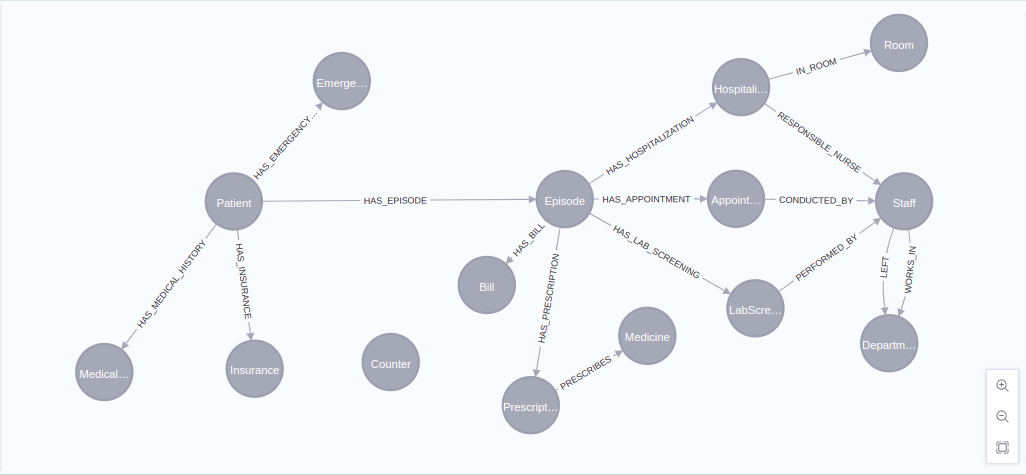
\includegraphics[width=0.95\linewidth]{Imagens/Neo4j/esquema_neo4j.png}
    \caption{Esquema da nossa base de dados Neo4j}
    \label{fig:esquema_neo4js}
\end{figure}

O esquema final no Neo4j inclui várias entidades (nós) e suas inter-relações, modelando de forma precisa o contexto hospitalar. A nossa estruturação de dados final têsm os 15 nós seguintes:

\begin{enumerate}
    \item \texttt{Paciente (Patient)}: Este nó representa todos os pacientes que já tiveram algum episódio hospitalar, exibindo os campos originais presentes na base de dados SQL. \ref{secPaciente}
    \item \texttt{Seguro de Saúde (Insurance)}: Este nó é representativo de vários seguros de saúde e contém os mesmos campos encontrados na tabela correspondente na base de dados SQL. \ref{secSeguroSaude}
    \item \texttt{Histórico Médico (Medical History)}: Este nó contém o histórico médico detalhado de cada paciente, mantendo os campos originais presentes na tabela SQL correspondente. \ref{secHistoricoMedico}
    \item \texttt{Contactos de Emergência (Emergency Contacts)}: Este nó representa os contactos de emergência dos pacientes, com os mesmos campos encontrados na tabela SQL correspondente. \ref{secContactosEmergencia}
    \item \texttt{Episódios Médicos (Episodes)}: Este nó é responsável por registar todos os episódios médicos de cada paciente, mantendo os campos originais da tabela correspondente presentes na base de dados SQL. \ref{secEpisodiosMedicos}
    \item \texttt{Faturas (Bill)}: Este nó representa as faturas associadas aos serviços prestados aos pacientes, mantendo os mesmos campos da tabela SQL correspondente. \ref{secFaturas}
    \item \texttt{Prescrição Médica (Prescription)}: Este nó contém informações sobre as prescrições médicas emitidas aos pacientes, mantendo a estrutura da tabela correspondente em SQL. \ref{secPrescricaoMedica}
    \item Medicamento (Medicine): Este nó representa os medicamentos disponíveis no hospital, mantendo os mesmos campos da tabela SQL correspondente. \ref{secMedicamento}
    \item \texttt{Departamento (Department)}: Este nó representa os diferentes departamentos do hospital, mantendo os parâmetros da tabela correspondente em SQL.\ref{secDepartamento}
    \item \texttt{Funcionários (Staff)}: Este nó reúne todas as tabelas referentes aos funcionários do nosso hospital, incluindo médicos, enfermeiros e técnicos. Dado que as estruturas das tabelas SQL para esses três tipos de funcionários são muito semelhantes, decidimos adotar uma abordagem semelhante ao MongoDB, abstraindo estas três tabelas e reunindo todos os elementos em um único nó denominado \texttt{staff}. Neste nó, apenas adicionamos um campo \texttt{role}, responsável por determinar a função do funcionário (DOCTOR, NURSE, TECHNICIAN). Para os funcionários com o papel de médico (\texttt{DOCTOR}), também adicionamos um campo \texttt{qualification}, característico da tabela \texttt{doctor} no SQL. \ref{secFuncionarios}
    \item \texttt{Consulta (Appointment):} Este nó regista as consultas marcadas pelos pacientes, mantendo os campos originais presentes na base de dados SQL. \ref{secConsulta}
    \item \texttt{Testes Médicos (Lab Screenings)}: Este nó contém informações sobre os testes médicos realizados nos pacientes, mantendo os mesmos campos da tabela SQL correspondente. \ref{secTestesMedicos}
    \item \texttt{Hospitalização (Hospitalization)}: Este nó regista informações sobre a hospitalização dos pacientes, mantendo os campos originais presentes na base de dados SQL. \ref{secHospitalizacao}
    \item \texttt{Quarto (Room)}: Este nó representa os quartos presentes no hospital. Os parâmetros deste nó são os mesmos da tabela correspondente na base de dados SQL.\ref{secQuarto}
    \item \texttt{Contador (Counter)}: Este nó auxiliar serve como um contador de IDs para os vários tipos de nós que possuem identificadores. Utilizando este nó, é possível obter um ID único sempre que um dos restantes tipos de nós seja adicionado, mantendo, desta forma, a integridade dos dados na base de dados Neo4j.\ref{secContador}
\end{enumerate}

No esquema final temos 16 relações entre os nós anteriormente mencionados. As relações são as seguintes:

\begin{enumerate}
    \item \texttt{HAS\_APPOINTMENT}: Representa a relação entre um paciente (\textit{patient}) e uma consulta agendada (\textit{appointment}). Um nó de paciente possui essa relação com um nó de consulta, indicando que o paciente tem uma consulta marcada.
    \item  \texttt{HAS\_BILL}: Reflete a relação entre um episódio médico (\textit{episode}) e uma fatura associada (\textit{bill}) a esse episódio. Um nó de episódio médico está conectado a um nó de fatura, indicando que ao episódio encontra-se associada uma fatura.
    \item  \texttt{HAS\_EMERGENCY\_CONTACT}: Indica a relação entre um paciente (\textit{patient}) e um contato de emergência (\textit{emergency contact}). Um nó de paciente está conectado a um ou mais nós de contato de emergência, representando que o paciente possui um ou mais contatos de emergência registados.
    \item  \texttt{HAS\_EPISODE}: Reflete a relação entre um paciente (\textit{patient}) e um episódio médico (\textit{episode}). Um nó de paciente possui essa relação com um nó de episódio médico, indicando que o paciente está envolvido nesse episódio e correlacionando assim o paciente com os elementos médicos.
    \item  \texttt{HAS\_HOSPITALIZATION}: Representa a relação entre um episódio médico (\textit{episode}) e uma hospitalização (\textit{hospitalization}) associada a esse episódio. Um nó de episódio médico está conectado a um nó de hospitalização, indicando que o episódio médico recorreu a uma hospitalização do paciente a qual o episódio se encontra associado.
    \item  \texttt{HAS\_INSURANCE}: Indica a relação entre um paciente (\textit{patient}) e um seguro de saúde (\textit{insurance}). Um nó de paciente possui essa relação com um nó de seguro de saúde, indicando qual o seguro de saúde do paciente em questão.
    \item  \texttt{HAS\_MEDICAL\_HISTORY}: Reflete a relação entre um paciente (\textit{patient}) e seu histórico médico (\textit{medical history}). Um nó de paciente está conectado a um ou mais nós de histórico médico, indicando que o paciente tem um ou mais nós de histórico médico registados.
    \item  \texttt{HAS\_PRESCRIPTION}: Denota a relação entre um episódio médico (\textit{episode}) e uma prescrição (\textit{prescription}) associada a esse episódio. Um nó de episódio médico está conectado a um ou mais nós de prescrição, indicando que o episódio possui uma ou mais prescrições.
    \item  \texttt{IN\_ROOM}: Representa a relação entre uma hospitalização (\textit{hospitalization}) e o quarto (\textit{room}) onde o paciente está internado. Um nó de hospitalização está conectado a um nó de quarto, indicando o quarto onde a hospitalização ocorre. Um nó de quarto pode ter associado várias hospitalizações desde que em horários que não coincidam.
    \item  \texttt{LEFT}: Indica a relação entre um paciente (\textit{patient}) e sua hospitalização (\textit{hospitalization}), semelhante ao que ocorre com a relação HAAS\_HOSPITALIZATION, no entanto, neste caso apenas os pacientes que já abandonaram uma hospitalização apresentam esta relação, ou seja, pacientes com alta hospitalar. Um nó de paciente possui essa relação com um nó de hospitalização, representando que o paciente teve alta do hospital.
    \item  \texttt{PRESCRIBES}: Reflete a relação entre um médico (\textit{doctor}) e uma prescrição (\textit{prescription}) que ele emite. Um nó de médico está conectado a um ou mais nós de prescrição, indicando que o médico emitiu a prescrição.
    \item  \texttt{RESPONSIBLE\_NURSE}: Indica a relação entre uma hospitalização (\textit{hospitalization}) e a enfermeira responsável (\textit{nurse}) por essa hospitalização. Um nó de hospitalização está conectado a um nó de enfermeira, representando que a enfermeira é responsável por essa hospitalização.
    \item  \texttt{CONDUCTED\_BY}: Representa a relação entre uma consulta agendada (\textit{appointment}) e o médico que a realizou. Um nó de consulta está conectado a um nó de médico, indicando que o médico conduziu a consulta.
    \item  \texttt{WORKS\_IN}: Denota a relação entre um funcionário (médico, enfermeiro, técnico) e o departamento (\textit{department}) em que ele trabalha. Um nó de funcionário possui essa relação com um nó de departamento, indicando que o funcionário trabalha no departamento.
    \item  \texttt{HAS\_LAB\_SCREENING}: Representa a relação entre um episódio médico (\textit{episode}) e um exame laboratorial (\textit{lab screening}) associado a esse episódio. Um nó de episódio médico está conectado a um ou mais nós de exame laboratorial, indicando que o episódio médico incluiu a realização de um ou mais exames exame.
    \item  \texttt{PERFORMED\_BY}: Reflete a relação entre um exame laboratorial (\textit{lab screening}) e um técnico (\textit{technician}) responsável por realizá-lo. Um nó de exame laboratorial está conectado a um nó de técnico, indicando que o técnico foi o responsável pela execução do exame laboratorial. O mesmo técnico pode ser responsável pela realização de vários exames laboratoriais.
\end{enumerate}

\section{\textit{Constraints} em Neo4j}

A migração de dados de Oracle para Neo4j envolveu a definição de várias \textit{constraints} para assegurar a integridade e a unicidade dos dados na base de dados orientada a grafos. As \textit{constraints} adicionadas garantem que os dados inseridos no Neo4j respeitam a unicidade dos ids, quando os mesmos existem, prevenindo duplicações e mantendo a consistência das informações armazenadas. A seguir, detalhamos as 14 \textit{constraints} implementadas:
\begin{enumerate}
    \item Pacientes (\textit{Patient}): Para garantir que cada paciente é único na base de dados, foi criada uma \textit{constraint} para assegurar a unicidade do identificador de paciente (\texttt{id\_patient}), assim, adicionamos uma \textit{constraint} ao identificador deste nó garantindo que não existem dois pacientes com o mesmo ID. 

    \begin{myminted}{cypher}
    CREATE CONSTRAINT FOR (p:Patient) REQUIRE p.id_patient IS UNIQUE
    \end{myminted}

    \item Seguros de Saúde (\textit{Insurance}): De modo a evitar duplicações nas apólices de seguro, foi adicionada uma constraint de unicidade para o número da apólice (policy\_number). 

    \begin{myminted}{cypher}
    CREATE CONSTRAINT FOR (i:Insurance) REQUIRE i.policy_number IS UNIQUE
    \end{myminted}
    
    \item Contatos de Emergência (\textit{Emergency Contact}): Para garantir que para este tipo de nó cada combinação de nome de contato, telefone e relação é única, foi criada uma \textit{constraint} composta incluindo estes três parâmetros.
    
    \begin{myminted}{cypher}
    CREATE CONSTRAINT unique_contact FOR (c:EmergencyContact) REQUIRE (c.contact_name, c.phone, c.relation) IS UNIQUE
    \end{myminted}
    
    \item Histórico Médico (\textit{Medical History}): Cada registo de histórico médico (\texttt{id\_record}) deve ser único para assegurar a integridade dos dados históricos dos pacientes, adicionamos, assim, uma \textit{constraint} no identificador deste nó como forma de garantir que não existem dois registos de histórico médico iguais.

    \begin{myminted}{cypher}
    CREATE CONSTRAINT FOR (m:MedicalHistory) REQUIRE m.id_record IS UNIQUE
    \end{myminted}
    
    \item Departamentos (\textit{Department}): Os departamentos são identificados de forma única pelo seu identificador de departamento (\texttt{id\_department}), ao colocarmos uma \textit{constraint} única no seu identificador garantimos que não é possível existir dois departamentos com o mesmo ID.
    
    \begin{myminted}{cypher}
    CREATE CONSTRAINT FOR (dep:Department) REQUIRE dep.id_department IS UNIQUE
    \end{myminted}

    \item Funcionários (\textit{Staff}): Para assegurar a unicidade dos funcionários na base de dados, foi adicionada uma \textit{constraint} no identificador do funcionário (\texttt{id\_emp}), desta forma garantimos que não existem dois funcionários com o mesmo ID.

    \begin{myminted}{cypher}
    CREATE CONSTRAINT FOR (s:Staff) REQUIRE s.id_emp IS UNIQUE
    \end{myminted}
    
    \item Quartos (\textit{Room}): Cada quarto ligado à hospitalização é identificado de forma única pelo seu identificador de quarto (\texttt{id\_room}), pelo que, apenas é necessário incluir uma \textit{constraint} neste identificador, garantindo que não existam dois quartos com o mesmo ID.

    \begin{myminted}{cypher}
    CREATE CONSTRAINT FOR (r:Room) REQUIRE r.id_room IS UNIQUE
    \end{myminted}
    
    \item Faturas (\textit{Bill}): As faturas são únicas e identificadas pelo seu identificador de fatura (\texttt{id\_bill}), assim sendo, apenas é necessário incluir uma \textit{constraint} neste identificador, garantindo que não existam duas faturas com o mesmo ID.
    
    \begin{myminted}{cypher}
    CREATE CONSTRAINT FOR (b:Bill) REQUIRE b.id_bill IS UNIQUE
    \end{myminted}
    
    \item Medicamentos (\textit{Medicine}): Cada medicamento é identificado de forma única pelo seu identificador de medicamento (\texttt{id\_medicine}), pelo que, apenas é necessário incluir uma \textit{constraint} neste identificador, garantindo que não existam dois medicamentos com o mesmo ID.
    
    \begin{myminted}{cypher}
    CREATE CONSTRAINT FOR (m:Medicine) REQUIRE m.id_medicine IS UNIQUE
    \end{myminted}
    
    \item Prescrições (\textit{Prescription}): De modo a evitar a existência de duplicações nas prescrições, foi criada uma constraint no identificador da prescrição (\texttt{id\_prescription}), garantindo que não existem duas prescrições com o mesmo ID.
    
    \begin{myminted}{cypher}
    CREATE CONSTRAINT FOR (p:Prescription) REQUIRE p.id_prescription IS UNIQUE  
    \end{myminted}
    
    \item Exames Laboratoriais (\textit{Lab Screening}): Cada exame laboratorial é identificado de forma única pelo seu identificador de exame (\texttt{id\_lab}), pelo que, apenas é necessário incluir uma \textit{constraint} neste identificador, garantindo que não existam dois exames laboratoriais com o mesmo ID.
    
    \begin{myminted}{cypher}
    CREATE CONSTRAINT FOR (l:LabScreening) REQUIRE l.id_lab IS UNIQUE
    \end{myminted}
    
    \item Consultas (\textit{Appointment}): Sendo que o nó não apresenta um identificador único, foi utilizado uma \textit{constraint} composta para garantir que as consultas são únicas. Uma consulta é identificadas pela combinação da data, hora e identificador do médico responsável, garantindo que um mesmo médico não pode dar duas consultas numa mesma data e hora. 
    
    \begin{myminted}{cypher}
    CREATE CONSTRAINT unique_appointment FOR (a:Appointment) REQUIRE(a.appointment_date, a.appointment_time, a.id_doctor) IS UNIQUE
    \end{myminted}
    
    \item Hospitalizações (\textit{Hospitalization}): Uma vez que este nó não apresenta um identificador único e para assegurar a unicidade das hospitalizações, foi criada uma \textit{constraint} composta que considera a data de admissão e o identificador do episódio médico, garantindo que duas hospitalizações na mesma data têm de ser feitas por episódios médicos diferentes, ou seja, para pacientes diferentes. 
    
    \begin{myminted}{cypher}
    CREATE CONSTRAINT unique_hospitalization FOR (h:Hospitalization) REQUIRE (h.admission_date, h.id_episode) IS UNIQUE
    \end{myminted}
    
    \item Episódios Médicos (\textit{Episode}): Cada episódio médico é identificado de forma única pelo seu identificador de episódio (\texttt{id\_episode}), pelo que apenas é necessário incluir uma \textit{constraint} neste identificador, garantindo que não existam dois episódios com o mesmo ID.
    
    \begin{myminted}{cypher}
    CREATE CONSTRAINT FOR (e:Episode) REQUIRE e.id_episode IS UNIQUE
    \end{myminted}
\end{enumerate}

\section{Triggers em Neo4j}

Durante o processo de migração de dados da base de dados Oracle para Neo4j, foi necessário definir diversos \textit{triggers} para otimizar a inserção de novos nós e manter a integridade dos dados. Na nossa base de dados, procurávamos evitar o uso manual de campos de identificação durante a inserção de novos nós. Para isso, utilizamos \textit{triggers} que gerassem automaticamente esses identificadores, garantindo a integridade e a unicidade dos dados.

Para alcançar este objetivo, introduzimos um nó auxiliar (\textit{Counter}) que armazena o número máximo dos identificadores utilizados até o momento. Este nó facilita a geração de novos identificadores únicos para futuros nós. Assim, após a inserção de um novo nó, os \textit{triggers} eram acionados para obter o próximo identificador a partir do nó \textit{Counter}, incrementar o contador presente neste nó, de acordo com o seu tipo, e atribuir o novo identificador ao nó recém-criado.

Além dos \textit{triggers} relacionados à criação de identificadores únicos, foi necessário adaptar um \textit{trigger} existente na base de dados original Oracle para o ambiente Neo4j. Este \textit{trigger} específico foi ajustado para garantir que sua funcionalidade fosse preservada após a migração, mantendo a consistência e a continuidade das operações automatizadas.

Em Neo4j, para a correta criação dos triggers, foi necessário recorrer à biblioteca \textbf{APOC} (\textit{Awesome Procedures on Cypher}). A biblioteca APOC fornece acesso a procedimentos e funções definidos pelos utilizadores que estendem o uso da linguagem de consulta \textit{Cypher} para novas áreas. Utilizando os recursos avançados oferecidos pela APOC, conseguimos automatizar e otimizar a criação e gestão de identificadores únicos para novos nós.

\subsection{Triggers para a adição de identificadores únicos}

Na sequencia da criação destes \textit{triggers} foi observado a existência de algumas consistências entre o nome do nó (\texttt{label}) e o nome do ID (\texttt{id\_ + label}). Estas consistências dividiram a implementação em dois tipos principais: \textit{triggers} dinâmicos para \textit{labels} comuns e \textit{triggers} específicos para \textit{labels} com nomes de identificador diferentes do nome da \textit{label}.

Os dados de transações em Neo4j são transformados em estruturas de dados apropriadas para serem consumidas como parâmetros nas instruções. Recorremos, portanto, à variável \texttt{\$createdNodes} que permite, quando um nó é criado no Neo4j, acionar o nosso \textit{trigger}. O parâmetro \texttt{\$createdNodes} é uma lista que contém os nós recém-criados durante a transação. Esta lista é então utilizada pelos \textit{triggers} para executar operações específicas, como, no nosso caso, a criação de identificadores únicos.

Assim sendo, para as \textit{labels}: \textit{Patient}, \textit{Room}, \textit{Department}, \textit{Episode}, \textit{Medicine}, \textit{Prescription} e \textit{Bill}, foi criado um único \textit{trigger} que fosse acionados com a inserção de nós das \textit{labels} mencionadas.

\begin{myminted}{cypher}
CALL apoc.trigger.install(
    'hospital',
    'dynamic_id_trigger',
    '
    UNWIND |\$|createdNodes AS n
    WITH n, head(apoc.node.labels(n)) AS label
    WITH n, label, \'id_\' + toLower(label) AS dynamicProperty
    WITH n, label, apoc.map.get(n, dynamicProperty, false) as idValue, dynamicProperty
    MATCH (c:Counter {type: label})
    WHERE label in ["Patient","Room","Department","Episode","Medicine","Prescription","Bill"] AND NOT idValue 
    CALL apoc.cypher.run("
        MATCH (c:Counter {type: |\$|label})
        RETURN c.count + 1 AS count
    ", {label: label}) YIELD value
    CALL apoc.create.setProperty(n, dynamicProperty, value.count) YIELD node
    SET n = node
    SET c.count = value.count
    ',
    {phase: 'afterAsync'}
);
\end{myminted}

Como podemos observar o procedimento seguido foi o seguinte:
\begin{enumerate}
    \item Instalar o \textit{trigger} denominado \texttt{dynamic\_id\_trigger} na base de dados \textbf{hospital}.
    \item Descompactar os nós criados (\textit{unwind}).
    \item Obter a \textit{label} que sofreu uma transação.
    \item Verifica se o nó não possui a propriedade do identificador (\texttt{apoc.map.get(n, dynamicProperty, false)}).
    \item Verifica se o nó é um dos nós onde existe uma consistência entre a \textit{label} e o nome do ID, só estes nós é que serão alterados com este \textit{trigger}.
    \item Incrementa o contador correspondente à \textit{label} e atribui o valor ao novo nó.
\end{enumerate}

Para os restantes \textit{triggers}, o processo é semelhante, a única diferença reside na forma como são identificados os nós e atribuídos os identificadores únicos. Cada \textit{trigger} é configurado para operar em um tipo específico de nó, verificando se esse nó já possui um identificador associado. Se não, é gerado um novo identificador único com base no contador (\textit{Counter}) correspondente ao tipo de nó. Esse identificador é então atribuído ao nó antes de atualizar o contador para refletir a adição do novo nó na base de dados. Assim, todos os \textit{triggers} garantem que os nós criados recebam identificadores únicos de forma automática e consistente, mantendo a integridade dos dados na base de dados Neo4j.

\subsection{Trigger proveniente da base de dados Oracle}

O \textit{trigger} proveniente da base de dados Oracle em questão têm como objetivo principal gerar automaticamente uma fatura (\textit{Bill}) quando um paciente recebe uma alta hospitalar, ou seja, quando ao nó hospitalização (\textit{hospitalization}), que é responsável por manter a informação sobre a hospitalização do paciente, é acrescentado o campo referente à data da alta hospitalar (\texttt{discharge\_date}). 

No ambiente Oracle, este \textit{trigger} era implementado para monitorizar a inserção do campo de alta hospitalar e, ao detetar essa inserção, iniciava uma série de processos para calcular os custos associados ao paciente durante sua estadia. Esses custos incluíam taxas de quarto (\texttt{room\_cost}), custos de exames laboratoriais (\texttt{test\_cost}) e outros encargos médicos (\texttt{other\_charges}). A soma total desses custos resultava na criação de uma nova fatura, que então era vinculada ao episódio de hospitalização do paciente.

Para a criação deste \textit{trigger} foi necessário recorrer à propriedade \texttt{\$assignedNodeProperties} da biblioteca \textit{apoc.trigger} para monitorizar mudanças nos nós. Esta propriedade é um mapa que contém chaves para listas de mapas, onde cada mapa inclui a chave \textit{(key)}, o valor antigo (\textit{old}), o valor novo (\textit{new}) e o nó (\textit{node}). O \textit{trigger} é ativado quando a propriedade \texttt{discharge\_date} é atribuída a um nó \textit{Hospitalization}.

O trigger obtido em Neo4j foi o seguinte:
\begin{myminted}{cypher}
    CALL apoc.trigger.install(
    'hospital',
    'trg_generate_bill',
    '
    UNWIND keys(\$assignedNodeProperties) AS k
    WITH k
    WHERE k = \'discharge_date\'
    UNWIND |\$|assignedNodeProperties[k] AS map
    WITH map.node AS h, map.old AS old, map.new AS new
    WHERE "Hospitalization" IN LABELS(h) AND old IS NULL AND new IS NOT NULL
    MATCH (e:Episode)-[:HAS_HOSPITALIZATION]->(h)
    MATCH (h)-[:IN_ROOM]->(r:Room)
    WITH e, h, COALESCE(r.room_cost, 0) AS v_room_cost
    OPTIONAL MATCH (e)-[:HAS_LAB_SCREENING]->(ls:LabScreening)
    WITH e, h, v_room_cost, COALESCE(SUM(ls.test_cost), 0) AS v_test_cost
    OPTIONAL MATCH (e)-[:HAS_PRESCRIPTION]->(p:Prescription)-[:PRESCRIBES]->(m:Medicine)
    WITH e, h, v_room_cost, v_test_cost, COALESCE(SUM(m.m_cost * p.dosage), 0) AS v_other_charges
    WITH e, v_room_cost, v_test_cost, v_other_charges, (v_room_cost + v_test_cost + v_other_charges) AS v_total_cost
    MATCH (c:Counter {type: \'Bill\'})
   CALL apoc.cypher.run("
        MATCH (c:Counter {type: \'Bill\'})
        RETURN c.count + 1 AS count
    ",{}) YIELD value
     CREATE (b:Bill {
        id_bill: value.count,
        room_cost: v_room_cost,
        test_cost: v_test_cost,
        other_charges: v_other_charges,
        total: v_total_cost,
        id_episode: e.id_episode,
        registered_at: datetime(),
        payment_status: "PENDING"
    })
    MERGE (e)-[:HAS_BILL]->(b)
    SET c.count = value.count
',
    {phase: 'afterAsync'}
);
\end{myminted}

O procedimento levado a cabo pelo \textit{trigger} apresentado acima é o seguinte:
\begin{enumerate}
    \item Instalação do \textit{trigger}.
    \item  Monitorização da Propriedade do nó de hospitalização, de forma a percecionar quando uum nó de hospitalização é atualizado com a inserção do campo \textit{discharge\_date} .
    \item  Cálculo de Custos associados com a hospitalização, recolhendo os custos do quarto associado à hospitalização (\texttt{\_room\_cost}), possíveis custos referentes à realização de testes laboratoriais (\texttt{v\_test\_cost}), e ainda possíveis despesas com a prescrição de medicação (\texttt{v\_other\_charges}). No final realizando o custo total da hospitalização, que estará presente na fatura, através da soma dos vários valores anteriormente referidos.
    \item  Criação de uma fatura (nó \textit{Bill}), recorrendo às variáveis, \texttt{v\_room\_cost}, \texttt{v\_test\_cost} e \texttt{v\_other\_charges}.
    \item  Associação da fatura ao episódio correspondente à hospitalização.
\end{enumerate}

Este trigger garante que a transição do OracleDB para o Neo4j mantenha a mesma eficiência e precisão na criação de faturas, assegurando a continuidade das operações financeiras no ambiente hospitalar de uma forma otimizada.

\section{Exploração da Base de Dados}

Após a migração para o Neo4J, conforme explicado anteriormente, iniciámos a exploração desta base de dados orientada a grafos. Para isso, utilizamos \textbf{queries} ou \textbf{expressões} tanto para passar um ID de uma tabela específica e obter a informação desejada, bem como, passar mais do que um parâmetro para obter dados de forma mais precisa e que englobassem mais do que um nó.

Por exemplo, para obter todas as informações de um paciente específico, incluindo detalhes sobre seus episódios médicos, consultas agendadas, faturas, hospitalizações e exames laboratoriais, utilizamos uma \textit{query} que recebe como parâmetro o \textit{id\_patient}. A \textit{query} percorre todos os nós que possuem estas informações apenas para o ID passado como parâmetro, fazendo uso das ligações entre eles para poder obter informação sobre cada um dos campos acima mencionados. Abaixo encontra-se a implementação desta \textit{query}:

\begin{myminted}{javascript}
MATCH (p:Patient {id_patient: 89})
OPTIONAL MATCH (p)-[:HAS_EPISODE]->(e:Episode)
OPTIONAL MATCH (e)-[:HAS_APPOINTMENT]->(appointment:Appointment)
OPTIONAL MATCH (e)-[:HAS_BILL]->(bill:Bill)
OPTIONAL MATCH (e)-[:HAS_HOSPITALIZATION]->(hospitalization:Hospitalization)
OPTIONAL MATCH (e)-[:HAS_LAB_SCREENING]->(lab:LabScreening)
RETURN p, 
       COLLECT(DISTINCT appointment) AS appointments, 
       COLLECT(DISTINCT bill) AS bills, 
       COLLECT(DISTINCT hospitalization) AS hospitalizations, 
       COLLECT(DISTINCT lab) AS labScreenings
\end{myminted}

Analisando a \textit{query} de forma concreta, temos:

\begin{myminted}{javascript}
MATCH (p:Patient {id_patient: 89})
\end{myminted}

Encontra o nó Patient com a campo \textit{id\_patient} igual a 89.

\begin{myminted}{javascript}
OPTIONAL MATCH (p)-[:HAS_EPISODE]->(e:Episode)
\end{myminted}

Realiza um \textit{match} opcional (que pode ou não existir) para encontrar todos os episódios médicos (\textit{Episode}) associados ao paciente. A relação \textit{HAS\_EPISODE} conecta o paciente aos seus episódios médicos.

\begin{myminted}{javascript}
OPTIONAL MATCH (e)-[:HAS_APPOINTMENT]->(appointment:Appointment)
\end{myminted}

Realiza um \textit{match} opcional para encontrar todas as consultas (\textit{Appointment}) associadas aos episódios médicos do paciente. A relação \textit{HAS\_APPOINTMENT} conecta os episódios médicos às suas consultas.

\begin{myminted}{javascript}
OPTIONAL MATCH (e)-[:HAS_BILL]->(bill:Bill)
\end{myminted}

Realiza um \textit{match} opcional para encontrar todas as faturas (\textit{Bill}) associadas aos episódios médicos do paciente. A relação \textit{HAS\_BILL} conecta os episódios médicos às suas faturas.

\begin{myminted}{javascript}
OPTIONAL MATCH (e)-[:HAS_HOSPITALIZATION]->(hospitalization:Hospitalization)
\end{myminted}

Realiza um \textit{match} opcional para encontrar todas as hospitalizações (\textit{Hospitalization}) associadas aos episódios médicos do paciente. A relação \textit{HAS\_HOSPITALIZATION} conecta os episódios médicos às suas hospitalizações.

\begin{myminted}{javascript}
OPTIONAL MATCH (e)-[:HAS_LAB_SCREENING]->(lab:LabScreening)
\end{myminted}

Realiza um \textit{match} opcional para encontrar todos os exames laboratoriais (\textit{LabScreening}) associados aos episódios médicos do paciente. A relação \textit{HAS\_LAB\_SCREENING} conecta os episódios médicos aos seus exames laboratoriais.

É importante mencionar que a utilização de uma base de dados orientada a grafos, como o Neo4j, oferece várias vantagens para o bom desempenho da \textit{query} fornecida. Vantagens como a \textbf{Consulta Rápida de Relacionamentos} que envolvem a navegação através de relações entre entidades, faz com que esta \textit{query} que envolve múltiplos relacionamentos (paciente para episódios, episódios para consultas, faturas, hospitalizações e exames), seja executada de forma muito eficiente. Outra vantagem que é importante mencionar é a \textbf{Travessia de Grafo} onde o Neo4J utiliza técnicas de travessia de grafo que permitem encontrar e retornar dados relacionados de forma rápida, mesmo com grandes volumes de dados.

\subsection{Operações Básicas em Neo4J}

Numa base de dados NoSQL como o Neo4J, não é necessário implementar funções separadas para realizar operações básicas como inserir, apagar ou atualizar nós. O Neo4J fornece métodos internos para lidar diretamente com estas operações. Aqui está um breve resumo de como pode realizar estas operações no Neo4J:

\begin{itemize}
    \item \textbf{Inserir Nós e Relacionamentos:} Para inserir um nó ou um relacionamento, pode usar-se o comando \texttt{CREATE}.
    \item \textbf{Apagar Nós e Relacionamentos:} Para apagar nós ou relacionamentos, pode usar-se o comando \texttt{DELETE}.
    \item \textbf{Atualizar Nós e Relacionamentos:} Para atualizar propriedades de nós ou relacionamentos, pode usar o comando \texttt{SET}. Para remover propriedades, pode usar o comando \texttt{REMOVE}.
\end{itemize}

O Neo4J, sendo uma base de dados NoSQL, é projetado para manipular dados de forma mais flexível e direta, eliminando a necessidade de mecanismos de controlo adicionais nas operações de \textbf{Criação} (\textit{CREATE}), \textbf{Atualização} (\textit{UPDATE}) e \textbf{Remoção} (\textit{DELETE}). 

\subsection{Visão Paciente}

\vspace{0.15cm} 
\textbf{Buscar todos os pacientes:} Esta query retorna todos os pacientes registados na base de dados. Cada paciente é representado por um nó \texttt{Patient}.

\vspace{0.15cm} 
\textbf{Buscar paciente por ID:} Retorna o nó \texttt{Patient} que tem um ID específico. Utiliza a propriedade \texttt{id\_patient} para encontrar o paciente desejado.

\vspace{0.15cm} 
\textbf{Buscar historial médico para um dado ID:} Retorna o nó \texttt{Patient} e todos os nós \texttt{MedicalHistory} relacionados a ele através da relação \texttt{HAS\_MEDICAL\_HISTORY}. Cada nó \texttt{MedicalHistory} contém informações sobre condições médicas passadas do paciente.

\vspace{0.15cm} 
\textbf{Buscar seguro para um dado ID:} Retorna os detalhes do seguro do paciente específico. Encontra o nó \texttt{Patient} com o ID fornecido e segue a relação \texttt{HAS\_INSURANCE} para obter o nó \texttt{Insurance} associado.

\vspace{0.15cm} 
\textbf{Buscar contacto de emergência para um dado ID:} Retorna os detalhes do contacto de emergência do paciente específico. Encontra o nó \texttt{Patient} com o ID fornecido e segue a relação \texttt{HAS\_EMERGENCY\_CONTACT} para obter o nó \texttt{EmergencyContact} associado.

\vspace{0.15cm} 
\textbf{Buscar pacientes por tipo de sangue:} Retorna todos os pacientes com um tipo de sangue específico. Utiliza a propriedade \texttt{blood\_type} do nó \texttt{Patient} para encontrar todos os pacientes com o tipo sanguíneo fornecido.

\vspace{0.15cm} 
\textbf{Buscar pacientes por género:} Retorna todos os pacientes de um género específico (masculino ou feminino). Utiliza a propriedade \texttt{gender} do nó \texttt{Patient} para filtrar os pacientes pelo género.

\vspace{0.15cm} 
\textbf{Buscar pacientes pela condição médica:} Retorna todos os pacientes que têm uma condição médica específica. Encontra todos os nós \texttt{Patient} que têm uma relação \texttt{HAS\_MEDICAL\_HISTORY} com um nó \texttt{MedicalHistory} onde a condição corresponde à fornecida.

\vspace{0.15cm} 
\textbf{Buscar todos os tipos de relações em contactos de emergência:} Retorna todos os tipos de relações registadas nos nós \texttt{EmergencyContact}. Cada relação descreve a natureza do contacto de emergência com o paciente (por exemplo, pai, mãe).

\vspace{0.15cm} 
\textbf{Buscar todos os tipos de provedores de seguro:} Retorna todos os provedores de seguro disponíveis na base de dados. Cada provedor é identificado pela propriedade \texttt{provider}.

\vspace{0.15cm} 
\textbf{Buscar todos os tipos de planos de seguro:} Retorna todos os diferentes planos de seguro registados nos nós \texttt{Insurance}. Cada plano é identificado pela propriedade \texttt{insurance\_plan}.

\vspace{0.15cm} 
\textbf{Buscar todos os tipos de cobertura:} Retorna todos os diferentes tipos de cobertura registados nos nós \texttt{Insurance}. Cada tipo de cobertura é identificado pela propriedade \texttt{coverage}.

\vspace{0.15cm} 
\textbf{Buscar historial médico:} Retorna todos os registros de historial médico na base de dados. Cada registro é representado por um nó \texttt{MedicalHistory}.

\vspace{0.15cm} 
\textbf{Buscar seguro:} Retorna todos os registros de seguro na base de dados. Cada registro é representado por um nó \texttt{Insurance}.

\vspace{0.15cm}
\textbf{Buscar contacto de emergência:} Retorna todos os registros de contactos de emergência na base de dados. Cada registro é representado por um nó \texttt{EmergencyContact}.

\vspace{0.15cm} 
\textbf{Buscar todos os tipos de condições médicas:} Retorna todos os diferentes tipos de condições médicas registadas nos nós \texttt{MedicalHistory}. Cada condição é identificada pela propriedade \texttt{condition}.

\vspace{0.15cm} 
\textbf{Buscar todos os tipos sanguíneos:} Retorna todos os diferentes tipos sanguíneos registados nos nós \texttt{Patient}. Cada tipo sanguíneo é identificado pela propriedade \texttt{blood\_type}.

\vspace{0.15cm} 
\textbf{Buscar número de pacientes para cada tipo sanguíneo:} Retorna o número de pacientes para cada tipo sanguíneo, ordenado pela quantidade de pacientes. Conta quantos nós \texttt{Patient} existem para cada valor de \texttt{blood\_type}.

\vspace{0.15cm} 
\textbf{Buscar número de pacientes para cada condição médica:} Retorna o número de pacientes para cada condição médica, ordenado pela quantidade de pacientes. Conta quantos nós \texttt{Patient} têm uma relação \texttt{HAS\_MEDICAL\_HISTORY} com um nó \texttt{MedicalHistory} para cada valor de \texttt{condition}.

\vspace{0.15cm} 
\textbf{Buscar pacientes por provedor de seguro específico:} Retorna todos os pacientes que têm seguro com um provedor específico. Encontra os nós \texttt{Patient} que têm uma relação \texttt{HAS\_INSURANCE} com um nó \texttt{Insurance} onde o provedor corresponde ao fornecido.

\vspace{0.15cm} 
\textbf{Buscar pacientes por plano de seguro específico:} Retorna todos os pacientes que têm um plano de seguro específico. Encontra os nós \texttt{Patient} que têm uma relação \texttt{HAS\_INSURANCE} com um nó \texttt{Insurance} onde o plano corresponde ao fornecido.

\vspace{0.15cm} 
\textbf{Buscar pacientes por cobertura específica:} Retorna todos os pacientes que têm uma cobertura de seguro específica. Encontra os nós \texttt{Patient} que têm uma relação \texttt{HAS\_INSURANCE} com um nó \texttt{Insurance} onde a cobertura corresponde à fornecida.

\vspace{0.15cm} 
\textbf{Buscar pacientes dentro de um intervalo de idades:} Retorna todos os pacientes nascidos entre datas específicas. Utiliza a propriedade \texttt{birthday} do nó \texttt{Patient} para filtrar os pacientes dentro do intervalo de datas fornecido.

\vspace{0.15cm}
\textbf{Buscar pacientes com cobertura de maternidade:} Retorna todos os pacientes que têm cobertura de maternidade no seguro. Encontra os nós \texttt{Patient} que têm uma relação \texttt{HAS\_INSURANCE} com um nó \texttt{Insurance} onde a cobertura de maternidade é verdadeira.

\vspace{0.15cm} 
\textbf{Buscar pacientes com cobertura dental:} Retorna todos os pacientes que têm cobertura dental no seguro. Encontra os nós \texttt{Patient} que têm uma relação \texttt{HAS\_INSURANCE} com um nó \texttt{Insurance} onde a cobertura dental é verdadeira.

\vspace{0.15cm} 
\textbf{Buscar pacientes com cobertura óptica:} Retorna todos os pacientes que têm cobertura óptica no seguro. Encontra os nós \texttt{Patient} que têm uma relação \texttt{HAS\_INSURANCE} com um nó \texttt{Insurance} onde a cobertura óptica é verdadeira.

\vspace{0.15cm} 
\textbf{Buscar pacientes com várias combinações de cobertura:} Retorna pacientes que têm várias combinações de coberturas (por exemplo, dental e óptica). Encontra os nós \texttt{Patient} que têm uma relação \texttt{HAS\_INSURANCE} com um nó \texttt{Insurance} onde múltiplas coberturas são verdadeiras.

\vspace{0.15cm} 
\textbf{Buscar pacientes por relação de contacto de emergência:} Retorna todos os pacientes cujo contacto de emergência tem uma relação específica (por exemplo, pai). Encontra os nós \texttt{Patient} que têm uma relação \texttt{HAS\_EMERGENCY\_CONTACT} com um nó \texttt{EmergencyContact} onde a relação corresponde à fornecida.

\vspace{0.15cm} 
\textbf{Buscar paciente pelo primeiro e último nome:} Retorna o paciente com um primeiro e último nome específico. Utiliza as propriedades \texttt{patient\_fname} e \texttt{patient\_lname} do nó \texttt{Patient} para encontrar o paciente.

\vspace{0.15cm} 
\textbf{Buscar paciente pelo número de telefone:} Retorna o paciente com um número de telefone específico. Utiliza a propriedade \texttt{phone} do nó \texttt{Patient} para encontrar o paciente.

\vspace{0.15cm} 
\textbf{Contar o número de pacientes:} Retorna a contagem total de pacientes registados na base de dados. Conta todos os nós \texttt{Patient}.

\vspace{0.15cm} 
\textbf{Buscar pacientes com um contacto de emergência específico:} Retorna todos os pacientes cujo contacto de emergência é uma pessoa específica. Encontra os nós \texttt{Patient} que têm uma relação \texttt{HAS\_EMERGENCY\_CONTACT} com um nó \texttt{EmergencyContact} onde o nome do contacto corresponde ao fornecido.

\vspace{0.15cm} 
\textbf{Buscar pacientes pelo ID do historial médico:} Retorna todos os pacientes que têm um historial médico com um ID específico. Encontra os nós \texttt{Patient} que têm uma relação \texttt{HAS\_MEDICAL\_HISTORY} com um nó \texttt{MedicalHistory} onde o ID do historial corresponde ao fornecido.

\subsection{Visão Staff}

\vspace{0.15cm}
\textbf{Buscar toda a Informação de um Staff:} Retorna todas as informações do funcionário cujo ID é fornecido. Utiliza a propriedade \texttt{id\_emp} para encontrar o funcionário desejado.

\vspace{0.15cm}
\textbf{Buscar o Department para um dado ID:} Retorna o funcionário com um ID específico e o departamento em que ele trabalha. Também pode buscar diretamente um departamento pelo seu ID.

\vspace{0.15cm}
\textbf{Buscar toda a informação das Enfermeiras:} Retorna todas as informações de todos os funcionários cujo papel é \textit{NURSE}. Utiliza a propriedade \texttt{role} para filtrar os funcionários.

\vspace{0.15cm}
\textbf{Buscar toda a informação dos Médicos:} Retorna todas as informações de todos os funcionários cujo papel é \textit{DOCTOR}. Utiliza a propriedade \texttt{role} para filtrar os funcionários.

\vspace{0.15cm}
\textbf{Buscar toda a informação dos Técnicos:} Retorna todas as informações de todos os funcionários cujo papel é \textit{TECHNICIAN}. Utiliza a propriedade \texttt{role} para filtrar os funcionários.

\vspace{0.15cm}
\textbf{Buscar quantos Enfermeiros existem:} Retorna a contagem de todos os funcionários cujo papel é \textit{NURSE}. Utiliza a propriedade \texttt{role} para contar os funcionários.

\vspace{0.15cm}
\textbf{Buscar quantos Doutores existem:} Retorna a contagem de todos os funcionários cujo papel é \textit{DOCTOR}. Utiliza a propriedade \texttt{role} para contar os funcionários.

\vspace{0.15cm}
\textbf{Buscar quantos Técnicos existem:} Retorna a contagem de todos os funcionários cujo papel é \textit{TECHNICIAN}. Utiliza a propriedade \texttt{role} para contar os funcionários.

\vspace{0.15cm}
\textbf{Buscar quantos enfermeiros, doutores e técnicos existem:} Retorna a contagem de funcionários agrupados por seus papéis (\textit{NURSE}, \textit{DOCTOR}, \textit{TECHNICIAN}). Utiliza a propriedade \texttt{role} para agrupar e contar os funcionários.

\vspace{0.15cm}
\textbf{Buscar quantos Departamentos existem:} Retorna a contagem de todos os departamentos na base de dados. Conta todos os nós \texttt{Department}.

\vspace{0.15cm}
\textbf{Buscar Staff por Data de Admissão:} Retorna todos os funcionários que foram admitidos na data fornecida. Utiliza a propriedade \texttt{date\_joining} para filtrar os funcionários.

\vspace{0.15cm}
\textbf{Buscar Staff por Data de Separação:} Retorna todos os funcionários que se separaram na data fornecida. Utiliza a propriedade \texttt{date\_separation} para filtrar os funcionários.

\vspace{0.15cm}
\textbf{Buscar Staff Ativo ou Inativo:} Retorna todos os funcionários que estão ativos ou inativos. Utiliza a propriedade \texttt{is\_active\_status} para filtrar os funcionários.

\vspace{0.15cm}
\textbf{Qualificações de um Doctor por ID:} Retorna as qualificações do doutor cujo ID é fornecido. Utiliza as propriedades \texttt{role} e \texttt{id\_emp} para encontrar o doutor.

\vspace{0.15cm}
\textbf{Todos os tipos de Qualificações:} Retorna todas as qualificações distintas dos doutores. Utiliza a propriedade \texttt{qualification} para listar as qualificações únicas.

\vspace{0.15cm}
\textbf{Número de Empregados por Departamento:} Retorna a contagem de funcionários por departamento. Utiliza a relação \texttt{WORKS\_IN} para agrupar e contar os funcionários por departamento.

\vspace{0.15cm}
\textbf{Enfermeiros por Departamento:} Retorna a contagem de enfermeiros por departamento. Utiliza a propriedade \texttt{role} e a relação \texttt{WORKS\_IN} para agrupar e contar os enfermeiros por departamento.

\vspace{0.15cm}
\textbf{Número de Doutores por Departamento:} Retorna a contagem de doutores por departamento. Utiliza a propriedade \texttt{role} e a relação \texttt{WORKS\_IN} para agrupar e contar os doutores por departamento.

\vspace{0.15cm}
\textbf{Número de Técnicos por Departamento:} Retorna a contagem de técnicos por departamento. Utiliza a propriedade \texttt{role} e a relação \texttt{WORKS\_IN} para agrupar e contar os técnicos por departamento.

\vspace{0.15cm}
\textbf{Contar Quantos Staff Estão Ativos:} Retorna a contagem de todos os funcionários que estão ativos. Utiliza a propriedade \texttt{is\_active\_status} para contar os funcionários ativos.

\vspace{0.15cm}
\textbf{Contar Quantos Staff não estão Ativos:} Retorna a contagem de todos os funcionários que não estão ativos. Utiliza a propriedade \texttt{is\_active\_status} para contar os funcionários inativos.

\vspace{0.15cm}
\textbf{Buscar Staff pelo Primeiro Nome e Sobrenome:} Retorna o funcionário cujo primeiro nome e sobrenome correspondem aos fornecidos. Utiliza as propriedades \texttt{emp\_fname} e \texttt{emp\_lname} para encontrar o funcionário.

\vspace{0.15cm}
\textbf{Buscar Staff pelo Email:} Retorna o funcionário cujo email corresponde ao fornecido. Utiliza a propriedade \texttt{email} para encontrar o funcionário.

\vspace{0.15cm}
\textbf{Contar o Número Total de Staff:} Retorna a contagem total de funcionários registados na base de dados. Conta todos os nós \texttt{Staff}.

\vspace{0.15cm}
\textbf{Buscar Staff pelo SSN:} Retorna o funcionário cujo número de segurança social (SSN) corresponde ao fornecido. Utiliza a propriedade \texttt{ssn} para encontrar o funcionário.

\subsection{Visão Episodes}

\vspace{0.15cm}
\textbf{Buscar toda a informação de um Episódio por ID:} Retorna todas as informações do episódio cujo ID é fornecido. Utiliza a propriedade \texttt{id\_episode} para encontrar o episódio desejado.

\vspace{0.15cm}
\textbf{Buscar toda a informação sobre Prescrições Hospitalares:} Retorna todas as informações de todas as prescrições registadas na base de dados.

\vspace{0.15cm}
\textbf{Quantos episódios para um dado paciente:} Retorna a contagem de episódios associados a um paciente específico. Utiliza a relação \texttt{HAS\_EPISODE} para contar os episódios de um paciente.

\vspace{0.15cm}
\textbf{Buscar as prescrições para um dado ID de episódio:} Retorna todas as prescrições associadas a um episódio específico. Utiliza a relação \texttt{HAS\_PRESCRIPTION} para obter as prescrições de um episódio.

\vspace{0.15cm}
\textbf{Buscar bill para um dado ID de episódio:} Retorna todas as contas associadas a um episódio específico. Utiliza a relação \texttt{HAS\_BILL} para obter as contas de um episódio.

\vspace{0.15cm}
\textbf{Buscar bill por ID de conta:} Retorna a conta cujo ID é fornecido. Utiliza a propriedade \texttt{id\_bill} para encontrar a conta desejada.

\vspace{0.15cm}
\textbf{Buscar exames laboratoriais para um dado ID de episódio:} Retorna todos os exames laboratoriais associados a um episódio específico. Utiliza a relação \texttt{HAS\_LAB\_SCREENING} para obter os exames de um episódio.

\vspace{0.15cm}
\textbf{Buscar exame laboratorial por ID de laboratório:} Retorna o exame laboratorial cujo ID é fornecido. Utiliza a propriedade \texttt{id\_lab} para encontrar o exame desejado.

\vspace{0.15cm}
\textbf{Buscar hospitalização para um dado ID de episódio:} Retorna todas as hospitalizações associadas a um episódio específico. Utiliza a relação \texttt{HAS\_HOSPITALIZATION} para obter as hospitalizações de um episódio.

\vspace{0.15cm}
\textbf{Buscar sala por ID de sala:} Retorna a sala cujo ID é fornecido. Utiliza a propriedade \texttt{id\_room} para encontrar a sala desejada.

\vspace{0.15cm}
\textbf{Buscar prescrições por ID de paciente:} Retorna todas as prescrições associadas a um paciente específico. Utiliza a propriedade \texttt{patient\_id} e a relação \texttt{HAS\_PRESCRIPTION} para obter as prescrições do paciente.

\vspace{0.15cm}
\textbf{Buscar bills por ID de paciente:} Retorna todas as contas associadas a um paciente específico. Utiliza a propriedade \texttt{patient\_id} e a relação \texttt{HAS\_BILL} para obter as contas do paciente.

\vspace{0.15cm}
\textbf{Buscar exames laboratoriais por ID de paciente:} Retorna todos os exames laboratoriais associados a um paciente específico. Utiliza a propriedade \texttt{patient\_id} e a relação \texttt{HAS\_LAB\_SCREENING} para obter os exames do paciente.

\vspace{0.15cm}
\textbf{Buscar hospitalização por ID de paciente:} Retorna todas as hospitalizações associadas a um paciente específico. Utiliza a propriedade \texttt{patient\_id} e a relação \texttt{HAS\_HOSPITALIZATION} para obter as hospitalizações do paciente.

\vspace{0.15cm}
\textbf{Buscar sala por ID de paciente:} Retorna todas as salas associadas a um paciente específico. Utiliza a propriedade \texttt{patient\_id}, a relação \texttt{HAS\_HOSPITALIZATION}, e a relação \texttt{IN\_ROOM} para obter as salas do paciente.

\vspace{0.15cm}
\textbf{Buscar medicamento por ID de paciente:} Retorna todos os medicamentos associados a um paciente específico. Utiliza a propriedade \texttt{patient\_id}, a relação \texttt{HAS\_PRESCRIPTION}, e a relação \texttt{PRESCRIBES} para obter os medicamentos do paciente.

\vspace{0.15cm}
\textbf{Buscar prescrições por ID de paciente e data:} Retorna todas as prescrições associadas a um paciente específico e uma data específica. Utiliza a propriedade \texttt{patient\_id}, a relação \texttt{HAS\_PRESCRIPTION}, e a propriedade \texttt{prescription\_date} para filtrar as prescrições.

\vspace{0.15cm}
\textbf{Buscar hospitalizações por ID de paciente e data de admissão:} Retorna todas as hospitalizações associadas a um paciente específico e uma data de admissão específica. Utiliza a propriedade \texttt{patient\_id}, a relação \texttt{HAS\_HOSPITALIZATION}, e a propriedade \texttt{admission\_date} para filtrar as hospitalizações.

\vspace{0.15cm}
\textbf{Buscar todas as prescrições de um paciente específico:} Retorna todas as prescrições de um paciente específico, independentemente do episódio. Utiliza a propriedade \texttt{patient\_id} e a relação \texttt{HAS\_PRESCRIPTION}.

\vspace{0.15cm}
\textbf{Buscar todas as contas de um paciente específico:} Retorna todas as contas de um paciente específico, independentemente do episódio. Utiliza a propriedade \texttt{patient\_id} e a relação \texttt{HAS\_BILL}.

\vspace{0.15cm}
\textbf{Buscar todos os exames laboratoriais de um paciente específico:} Retorna todos os exames laboratoriais de um paciente específico, independentemente do episódio. Utiliza a propriedade \texttt{patient\_id} e a relação \texttt{HAS\_LAB\_SCREENING}.

\vspace{0.15cm}
\textbf{Buscar todas as hospitalizações de um paciente específico:} Retorna todas as hospitalizações de um paciente específico, independentemente do episódio. Utiliza a propriedade \texttt{patient\_id} e a relação \texttt{HAS\_HOSPITALIZATION}.

\vspace{0.15cm}
\textbf{Buscar todas as salas de um paciente específico:} Retorna todas as salas de um paciente específico, independentemente do episódio. Utiliza a propriedade \texttt{patient\_id}, a relação \texttt{HAS\_HOSPITALIZATION}, e a relação \texttt{IN\_ROOM}.

\vspace{0.15cm}
\textbf{Buscar todas as informações de um episódio específico:} Retorna todas as informações detalhadas de um episódio específico, incluindo prescrições, contas, hospitalizações e exames laboratoriais. Utiliza a propriedade \texttt{id\_episode} para encontrar o episódio e suas relações associadas.

\vspace{0.15cm}
\textbf{Buscar todas as informações de todos os episódios:} Retorna todas as informações detalhadas de todos os episódios, incluindo prescrições, contas, hospitalizações e exames laboratoriais. Utiliza as relações associadas aos episódios.

\vspace{0.15cm}
\textbf{Buscar informações do médico responsável por um episódio específico:} Retorna todas as informações do médico responsável por um episódio específico. Utiliza a relação \texttt{HAS\_APPOINTMENT} e a relação \texttt{CONDUCTED\_BY} para obter o médico.

\vspace{0.15cm}
\textbf{Buscar todas as informações dos médicos que atenderam um paciente específico:} Retorna todas as informações dos médicos que atenderam um paciente específico. Utiliza a relação \texttt{HAS\_EPISODE}, a relação \texttt{HAS\_APPOINTMENT}, e a relação \texttt{CONDUCTED\_BY} para obter os médicos.

\vspace{0.15cm}
\textbf{Buscar informações do técnico responsável por um episódio específico:} Retorna todas as informações do técnico responsável por um episódio específico. Utiliza a relação \texttt{HAS\_LAB\_SCREENING} e a relação \texttt{PERFORMED\_BY} para obter o técnico.

\vspace{0.15cm}
\textbf{Buscar todas as informações dos técnicos que atenderam um paciente específico:} Retorna todas as informações dos técnicos que atenderam um paciente específico. Utiliza a relação \texttt{HAS\_EPISODE}, a relação \texttt{HAS\_LAB\_SCREENING}, e a relação \texttt{PERFORMED\_BY} para obter os técnicos.

\vspace{0.15cm}
\textbf{Retornar informações de um paciente específico dado um ID de paciente:} Retorna todas as informações de um paciente específico, incluindo todos os episódios, consultas, contas, hospitalizações e exames laboratoriais. Utiliza a propriedade \texttt{id\_patient} e as relações associadas.

\vspace{0.15cm}
\textbf{Retornar informações de todos os pacientes:} Retorna todas as informações detalhadas de todos os pacientes, incluindo todos os episódios, consultas, contas, hospitalizações e exames laboratoriais. Utiliza as relações associadas aos pacientes.

\subsection{Visão Global}

\vspace{0.15cm}
\textbf{Listar todas as prescrições para um paciente específico:} Retorna todas as prescrições associadas a um paciente específico. Utiliza a relação \texttt{HAS\_EPISODE} para encontrar os episódios do paciente e a relação \texttt{HAS\_PRESCRIPTION} para obter as prescrições desses episódios.

\vspace{0.15cm}
\textbf{Listar os pacientes alocados a um específico quarto:} Retorna todos os pacientes que estão alocados a um quarto específico. Utiliza a relação \texttt{IN\_ROOM} para encontrar as hospitalizações no quarto e a relação \texttt{HAS\_HOSPITALIZATION} para obter os episódios associados aos pacientes.

\vspace{0.15cm}
\textbf{Listar todos os internamentos de um determinado paciente:} Retorna todas as hospitalizações associadas a um paciente específico. Utiliza a relação \texttt{HAS\_EPISODE} para encontrar os episódios do paciente e a relação \texttt{HAS\_HOSPITALIZATION} para obter as hospitalizações desses episódios.

\vspace{0.15cm}
\textbf{Listar hospitalizações por enfermeira responsável:} Retorna todas as hospitalizações pelas quais uma enfermeira específica é responsável. Utiliza a relação \texttt{RESPONSIBLE\_NURSE} para encontrar as hospitalizações associadas ao enfermeiro.

\vspace{0.15cm}
\textbf{Listar todos os episódios médicos de um paciente específico:} Retorna todos os episódios médicos associados a um paciente específico. Utiliza a relação \texttt{HAS\_EPISODE} para encontrar os episódios do paciente.

\vspace{0.15cm}
\textbf{Listar episódios médicos por tipo de condição:} Retorna todos os episódios médicos associados a pacientes com uma condição médica específica. Utiliza a relação \texttt{HAS\_MEDICAL\_HISTORY} para encontrar os pacientes com a condição e a relação \texttt{HAS\_EPISODE} para obter os episódios desses pacientes.

\vspace{0.15cm}
\textbf{Listar todos os episódios médicos tratados por um médico específico:} Retorna todos os episódios médicos tratados por um médico específico. Utiliza a relação \texttt{CONDUCTED\_BY} para encontrar as consultas conduzidas pelo médico e a relação \texttt{HAS\_APPOINTMENT} para obter os episódios associados a essas consultas.

\vspace{0.15cm}
\textbf{Listar todos os exames laboratoriais para um paciente específico:} Retorna todos os exames laboratoriais associados a um paciente específico. Utiliza a relação \texttt{HAS\_EPISODE} para encontrar os episódios do paciente e a relação \texttt{HAS\_LAB\_SCREENING} para obter os exames desses episódios.

\vspace{0.15cm}
\textbf{Listar exames baseados no técnico responsável:} Retorna todos os exames laboratoriais realizados por um técnico específico. Utiliza a relação \texttt{PERFORMED\_BY} para encontrar os exames associados ao técnico.

\vspace{0.15cm}
\textbf{Listar todas as faturas para um paciente específico:} Retorna todas as faturas associadas a um paciente específico. Utiliza a relação \texttt{HAS\_EPISODE} para encontrar os episódios do paciente e a relação \texttt{HAS\_BILL} para obter as faturas desses episódios.

\vspace{0.15cm}
\textbf{Listar todas as consultas agendadas para um paciente específico:} Retorna todas as consultas agendadas associadas a um paciente específico. Utiliza a relação \texttt{HAS\_EPISODE} para encontrar os episódios do paciente e a relação \texttt{HAS\_APPOINTMENT} para obter as consultas desses episódios.

\vspace{0.15cm}
\textbf{Listar consultas baseadas no médico responsável:} Retorna todas as consultas conduzidas por um médico específico. Utiliza a relação \texttt{CONDUCTED\_BY} para encontrar as consultas associadas ao médico.

\vspace{0.15cm}
\textbf{Listar os Appointment para um dado Medico por dia:} Retorna todas as consultas agendadas para um médico específico em uma data específica. Utiliza a relação \texttt{CONDUCTED\_BY} e filtra pela data da consulta.

\vspace{0.15cm}
\textbf{Buscar Appointment por data:} Retorna todas as consultas agendadas em uma data específica. Utiliza a propriedade \texttt{appointment\_date} para filtrar as consultas.

\vspace{0.15cm}
\textbf{Buscar Appointment por data e depois por hora:} Retorna todas as consultas agendadas em uma data e hora específicas. Utiliza as propriedades \texttt{appointment\_date} e \texttt{appointment\_time} para filtrar as consultas.

\vspace{0.15cm}
\textbf{Lista todos os episódios e o respetivo paciente:} Retorna todos os episódios médicos e os pacientes associados. Utiliza a relação \texttt{HAS\_EPISODE} para obter os episódios e os pacientes correspondentes.

\vspace{0.15cm}
\textbf{Lista os médicos com mais consultas marcadas, com informação detalhada do paciente:} Retorna os médicos com mais consultas marcadas, incluindo informações detalhadas dos pacientes atendidos. Utiliza a relação \texttt{CONDUCTED\_BY} para encontrar as consultas, agrupa os médicos pelo número de consultas e coleta informações dos pacientes atendidos.

\chapter{Análise Crítica}
\paragraph{}

% Ao longo do projeto, desenvolvemos a migração de dados de um sistema de gestão hospitalar baseado em \textbf{Oracle SQL} para sistemas NoSQL, especificamente \textbf{MongoDB} e \textbf{Neo4j}. Esta migração foi crucial para atender às crescentes demandas e complexidades dos dados modernos, proporcionando maior flexibilidade e escalabilidade.

%Ao nível da exploração, esta foi levada ao detalhe. Ao longo de todo o projeto, para cada uma das bases de dados — relacional, orientada a documentos ou orientada a grafos — desenvolvemos todas as queries, funções e outras operações de forma a serem utilizadas e aplicadas no contexto real de um centros hospitalares.

%Esforçámo-nos por garantir que estas ferramentas pudessem ser usadas eficazmente tanto pelos pacientes, através da utilização de perfis personalizados, como pelo staff hospitalar para a gestão de informações e operações diárias. Adicionalmente, desenvolvemos funcionalidades específicas para a gestão de episódios médicos, tanto os que estão a decorrer como os já passados, assegurando uma administração eficiente e integrada dos dados hospitalares.

%Este nível de detalhe na exploração permitiu-nos criar um sistema robusto e versátil, capaz de atender às necessidades de diversos utilizadores num ambiente hospitalar real.

%Durante o desenvolvimento, enfrentámos diversos desafios, como a manutenção da integridade dos dados e a adaptação de triggers. Para resolver esses problemas, utilizámos a biblioteca APOC em Neo4j para a criação de triggers e definimos constraints para garantir a unicidade dos dados.

%- Falar da extensão exploração realizada em cada um das DB

%- Falar dos Triggers em mais detalhe

%- Falar do Counter

%- Falar das Datas?!

Ao longo deste projeto, realizámos a migração de dados de um sistema de gestão hospitalar baseado em Oracle SQL para sistemas NoSQL, nomeadamente MongoDB e Neo4j. Esta migração revelou-se essencial para responder às crescentes exigências e complexidades dos dados modernos, oferecendo maior flexibilidade e escalabilidade.

A exploração das bases de dados foi conduzida de forma meticulosa. Para cada uma das bases de dados — relacional, orientada a documentos ou orientada a grafos — desenvolvemos consultas, funções e outras operações de modo a serem aplicáveis no contexto real de um hospital. Em MongoDB, implementámos várias funções e expressões para obter informações detalhadas e gerais. Em Neo4j, as consultas foram otimizadas para obter dados complexos de forma eficiente.

Procurámos garantir que estas ferramentas pudessem ser usadas de forma eficaz tanto pelos pacientes, através de perfis personalizados, como pelo pessoal hospitalar para a gestão de informações e operações diárias. Adicionalmente, desenvolvemos funcionalidades específicas para a gestão de episódios médicos, tanto os que estão a decorrer como os já finalizados, assegurando uma administração eficiente e integrada dos dados hospitalares.

Este nível de detalhe na exploração permitiu-nos criar um sistema robusto e versátil, capaz de atender às necessidades de diversos utilizadores num ambiente hospitalar real.

Durante o desenvolvimento, enfrentámos vários desafios, como a manutenção da integridade dos dados e a adaptação de \textit{triggers}. Os \textit{triggers} desempenharam um papel crucial na manutenção da integridade dos dados e na automatização de processos. A criação de \textit{triggers} em Neo4j, com o auxílio da biblioteca APOC, e em MongoDB, recorrendo à ferramenta Atlas, foi fundamental para a geração automática de identificadores únicos e a preservação da consistência dos dados.

Introduzimos também um nó auxiliar (\textit{Counter}) e uma coleção auxiliar (\textit{counters}) cuja principal função é armazenar o número máximo dos identificadores utilizados até ao momento. Estas duas abordagens facilitaram a geração de novos identificadores únicos para futuros elementos das nossas bases de dados. A gestão de datas foi abordada com cuidado para garantir a precisão e a consistência dos registos temporais nos diferentes sistemas de bases de dados.
\chapter{Conclusão}
\paragraph{}

% Em suma, este trabalho representou uma valiosa contribuição para aprofundar nosso conhecimento sobre a área de migração de dados e exploração de bases de dados NoSQL, oferecendo uma visão prática das estratégias e desafios envolvidos. Para trabalhos futuros, sugerimos a otimização contínua das consultas, a expansão das funcionalidades do sistema, como, por exemplo, a inclusão mais do que uma unidade hospitalar.

% Foi possível observar que a flexibilidade e escalabilidade dos sistemas NoSQL proporcionaram uma gestão mais eficiente dos dados, especialmente em termos de consultas e operações complexas. A utilização da biblioteca APOC em Neo4j e a definição de \textit{constraints} foram essenciais para manter a integridade dos dados durante a migração. Além disso, as consultas implementadas demonstraram capacidades operacionais superiores em comparação com o sistema relacional original, facilitando a obtenção de informações detalhadas.

% Para trabalhos futuros, sugerimos a otimização contínua das consultas para melhorar ainda mais o desempenho do sistema. Além disso, a expansão das funcionalidades do sistema pode abranger a integração de novos tipos de dados, a implementação de novos \textit{triggers}, e a melhoria das interfaces de consulta. Adicionalmente, a aplicação dos conhecimentos adquiridos em outros domínios de dados pode oferecer \textit{insights} valiosos para a construção de sistemas similares. Esta abordagem poderá contribuir para o desenvolvimento de soluções mais robustas e adaptáveis às necessidades específicas de diferentes indústrias.

O trabalho realizado sobre a migração e exploração de bases de dados NoSQL representou um avanço significativo no conhecimento e aplicação dessas tecnologias em ambientes hospitalares. A migração de um sistema baseado em Oracle SQL para MongoDB e Neo4j não só demonstrou a viabilidade e os benefícios dos sistemas NoSQL, como também ofereceu \textit{insights} práticos sobre as estratégias e desafios enfrentados.

Observou-se que a flexibilidade e escalabilidade dos sistemas NoSQL proporcionaram uma gestão de dados mais eficiente, particularmente em consultas e operações complexas. Em relação ao MongoDB a utilização da ferramenta Atlas foi essencial para a criação de \textit{triggers} essenciais ao nosso modelo de dados. Quanto a Neo4j a utilização da biblioteca APOC e a definição de \textit{constraints} foram cruciais para manter a integridade dos dados durante a migração. Além disso, as consultas implementadas exibiram capacidades operacionais superiores em comparação com o sistema relacional original, facilitando a obtenção de informações detalhadas.

Para futuros trabalhos, recomenda-se a otimização contínua das consultas para aprimorar ainda mais o desempenho do sistema. A expansão das funcionalidades do sistema pode incluir a integração de novos tipos de dados, a implementação de novos \textit{triggers}, e a melhoria das interfaces de consulta. 

Esta abordagem não apenas reforça a versatilidade e a capacidade dos sistemas NoSQL, mas também destaca a importância de um contínuo processo de inovação e adaptação às demandas crescentes e complexas dos dados modernos, particularmente em contextos críticos como o hospitalar.
\appendix

\chapter{Nodos desenvolvidos em Neo4J}

%\begin{appendices}

\section{Paciente}\label{secPaciente}
\begin{figure}[H]
    \centering
    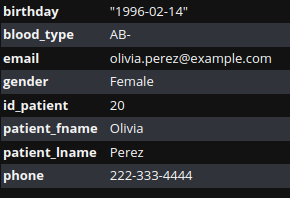
\includegraphics[width=0.3\linewidth]{Imagens/Neo4j/patient.png}
    \caption{Exemplo de um nodo paciente}
    \label{fig:nodo_paciente}
\end{figure}

\section{Seguro de Saúde}\label{secSeguroSaude}
\begin{figure}[H]
    \centering
    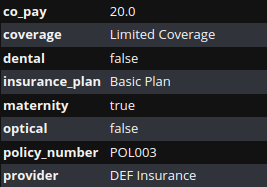
\includegraphics[width=0.3\linewidth]{Imagens/Neo4j/insurance.png}
    \caption{Exemplo de um nodo seguro de saúde}
    \label{fig:nodo_seguro_saude}
\end{figure}

\section{Histórico médico}\label{secHistoricoMedico}
\begin{figure}[H]
    \centering
    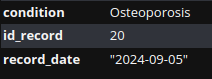
\includegraphics[width=0.3\linewidth]{Imagens/Neo4j/medical_history.png}
    \caption{Exemplo de um nodo histórico médico}
    \label{fig:nodo_historico_medico}
\end{figure}

\section{Contactos de Emergência}\label{secContactosEmergencia}
\begin{figure}[H]
    \centering
    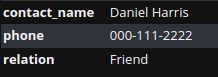
\includegraphics[width=0.3\linewidth]{Imagens/Neo4j/emergency_contact.png}
    \caption{Exemplo de um nodo contactos de emergência}
    \label{fig:nodo_contactos_emergencia}
\end{figure}

\section{Episódios Médicos}\label{secEpisodiosMedicos}
\begin{figure}[H]
    \centering
    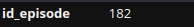
\includegraphics[width=0.3\linewidth]{Imagens/Neo4j/episode.png}
    \caption{Exemplo de um nodo episódios médicos}
    \label{fig:nodo_episodios_medicos}
\end{figure}

\section{Faturas}\label{secFaturas}
\begin{figure}[H]
    \centering
    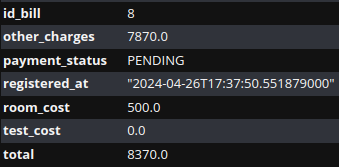
\includegraphics[width=0.3\linewidth]{Imagens/Neo4j/bill.png}
    \caption{Exemplo de um nodo faturas}
    \label{fig:nodo_faturas}
\end{figure}

\section{Prescrição Médica}\label{secPrescricaoMedica}
\begin{figure}[H]
    \centering
    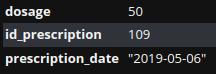
\includegraphics[width=0.3\linewidth]{Imagens/Neo4j/prescription.png}
    \caption{Exemplo de um nodo prescrição médica}
    \label{fig:nodo_prescricao_medica}
\end{figure}

\section{Medicamento}\label{secMedicamento}
\begin{figure}[H]
    \centering
    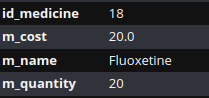
\includegraphics[width=0.3\linewidth]{Imagens/Neo4j/medicine.png}
    \caption{Exemplo de um nodo medicamento}
    \label{fig:nodo_medicamento}
\end{figure}

\section{Departamento}\label{secDepartamento}
\begin{figure}[H]
    \centering
    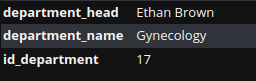
\includegraphics[width=0.3\linewidth]{Imagens/Neo4j/department.png}
    \caption{Exemplo de um nodo departamento}
    \label{fig:nodo_departamento}
\end{figure}

\section{Funcionários}\label{secFuncionarios}
\begin{figure}[H]
    \centering
    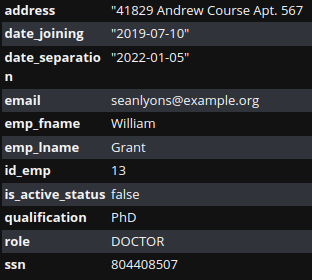
\includegraphics[width=0.3\linewidth]{Imagens/Neo4j/staff.png}
    \caption{Exemplo de um nodo funcionários}
    \label{fig:nodo_funcionarios}
\end{figure}

\section{Consulta}\label{secConsulta}
\begin{figure}[H]
    \centering
    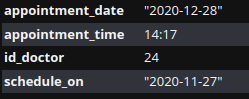
\includegraphics[width=0.3\linewidth]{Imagens/Neo4j/appointment.png}
    \caption{Exemplo de um nodo consulta}
    \label{fig:nodo_consulta}
\end{figure}

\section{Testes Médicos}\label{secTestesMedicos}
\begin{figure}[H]
    \centering
    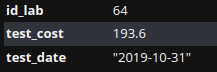
\includegraphics[width=0.3\linewidth]{Imagens/Neo4j/lab_screening.png}
    \caption{Exemplo de um nodo testes médicos}
    \label{fig:nodo_testes_medicos}
\end{figure}

\section{Hospitalização}\label{secHospitalizacao}
\begin{figure}[H]
    \centering
    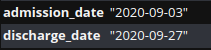
\includegraphics[width=0.3\linewidth]{Imagens/Neo4j/hospitalization.png}
    \caption{Exemplo de um nodo hospitalização}
    \label{fig:nodo_hospitalizacao}
\end{figure}

\section{Quarto}\label{secQuarto}
\begin{figure}[H]
    \centering
    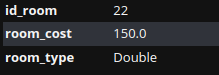
\includegraphics[width=0.3\linewidth]{Imagens/Neo4j/room.png}
    \caption{Exemplo de um nodo quarto}
    \label{fig:nodo_quarto}
\end{figure}

\section{Contador}\label{secContador}
\begin{figure}[H]
    \centering
    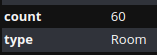
\includegraphics[width=0.3\linewidth]{Imagens/Neo4j/counter.png}
    \caption{Exemplo de um nodo contador}
    \label{fig:nodo_contador}
\end{figure}


%\end{appendices}


\end{document}